\documentclass[12pt,a4paper,openany]{book}
\usepackage[utf8]{inputenc}
\usepackage[T1]{fontenc}
\usepackage[italian]{babel}
\usepackage{graphicx}
\usepackage{float}
\usepackage{geometry}
\usepackage[colorlinks=true, linkcolor=black, urlcolor=blue, citecolor=black]{hyperref}
\usepackage{amsmath}
\usepackage{amssymb}
\usepackage{microtype}
\usepackage{parskip}
\usepackage{booktabs}
\usepackage{lmodern}
\usepackage{caption}
\usepackage{subcaption}
\usepackage{array}
\usepackage{tabularx}
\usepackage{fancyhdr}
\usepackage{emptypage}
\usepackage[titles]{tocloft}

\geometry{
  a4paper,
  top=3cm, bottom=3cm,
  inner=3cm, outer=2.5cm,
  headheight=27.2pt   % <-- aumentato per eliminare i warning
}

\addtolength{\topmargin}{-2pt} % compensa l'incremento di headheight

% Header/footer style
\pagestyle{fancy}
\fancyhf{}
\fancyhead[LE,RO]{\thepage}
\fancyhead[RE]{\textit{\leftmark}}
\fancyhead[LO]{\textit{\rightmark}}
\renewcommand{\headrulewidth}{0.4pt}

% Caption style
\captionsetup{font=small, labelfont=bf, margin=1cm}

% Nicer figure placement
\setcounter{topnumber}{3}
\setcounter{bottomnumber}{2}
\setcounter{totalnumber}{4}
\renewcommand{\topfraction}{0.85}
\renewcommand{\bottomfraction}{0.5}
\renewcommand{\textfraction}{0.15}
\renewcommand{\floatpagefraction}{0.7}

\title{\textbf{Sbobine di Elettrofisiologia Cellulare}}
\author{}
\date{\today}

\begin{document}
\frontmatter
\maketitle
\tableofcontents

\mainmatter

\chapter{Richiami di elettrofisiologia cellulare}

\section{1a. Struttura del neurone, potenziale di membrana, meccanismi di trasporto}

\subsection{La cellula nervosa}

Il sistema nervoso è ciò che distingue un animale e un non animale, la componente cellulare principale di tale sistema è il neurone (cellula nervosa).

Alla cellula nervosa sono associate tre funzioni principali. Il neurone, oltre a trasmettere impulsi, è considerato un ``piccolo centro di calcolo'' che svolge in maniera ridotta quello che fa il cervello.

\begin{itemize}
  \item la ricezione delle informazioni, da altre cellule o da ricettori, avviene nell'albero dendritico. Gli stimoli che pervengono sono molteplici infatti la cellula è dotata di più ingressi.
\end{itemize}
\begin{figure}[htbp]
  \centering
  
\includegraphics[width=0.80\textwidth]{images/image1.png}
\end{figure}

\begin{itemize}
  \item \textbf{Integrazione:} le informazioni ricevute in ingresso devono essere elaborate (processo di integrazione). A tanti ingressi corrisponde una sola uscita (assone), tramite un meccanismo a soglia: se viene raggiunto il livello soglia la cellula genera un impulso, altrimenti ritorna all'equilibrio. L'integrazione è distribuita su tutta la membrana, sul soma e sull'albero dendritico, tranne che sull'assone.
  \item \textbf{Generazione e propagazione:} l'impulso (treno di potenziali d'azione) raggiunge altre cellule o gli attuatori, come la cellula muscolare, mettendo in pratica la decisione elaborata.
\end{itemize}

\begin{figure}[htbp]
  \centering
  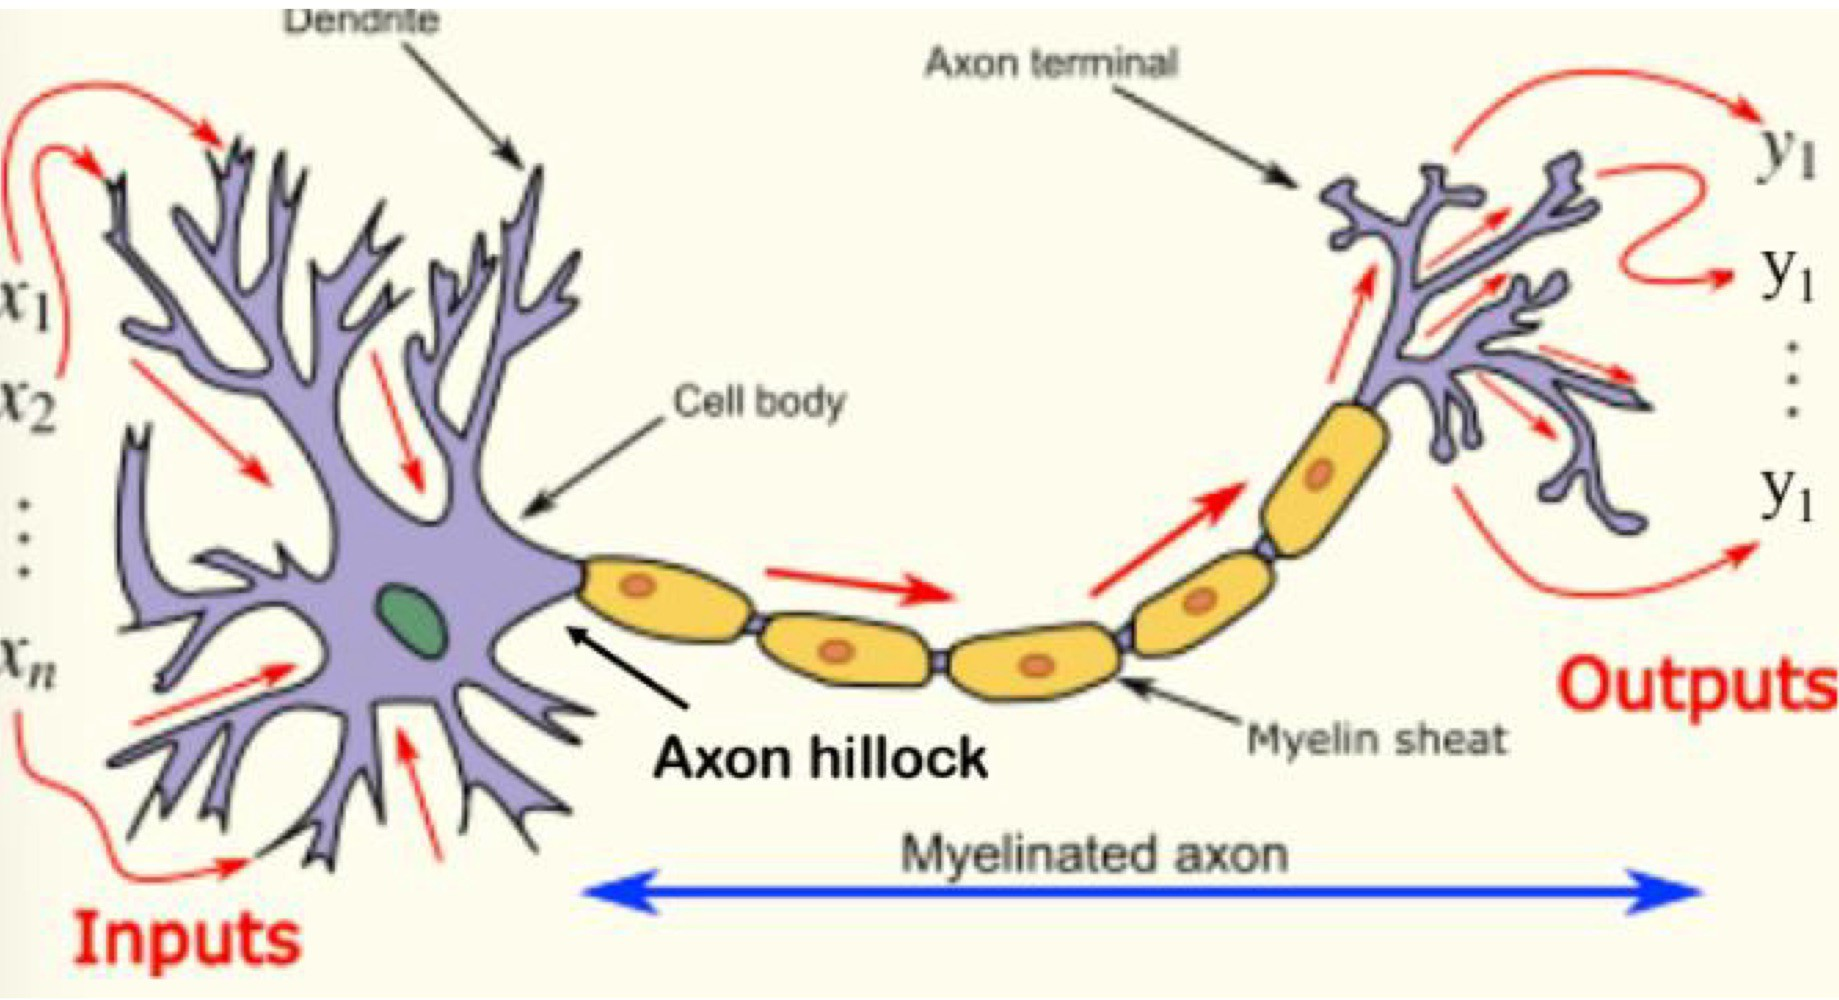
\includegraphics[width=0.80\textwidth]{images/image8.jpeg}
\end{figure}

Generazione e propagazione: l'impulso (generato principalmente sul cono di emergenza dell'assone) è unidirezionale, parte dal soma, si propaga lungo l'assone e arriva alle sinapsi, dove viene trasmessa. La parte finale dell'assone che prende il nome di bottone sinaptico porta sempre lo stesso segnale.

La struttura delle cellule nervose non è sempre la stessa, in particolare ciò che cambia è la forma, le componenti sono le stesse.


\subsection{Struttura della membrana neuronale}

\begin{figure}[htbp]
  \centering
  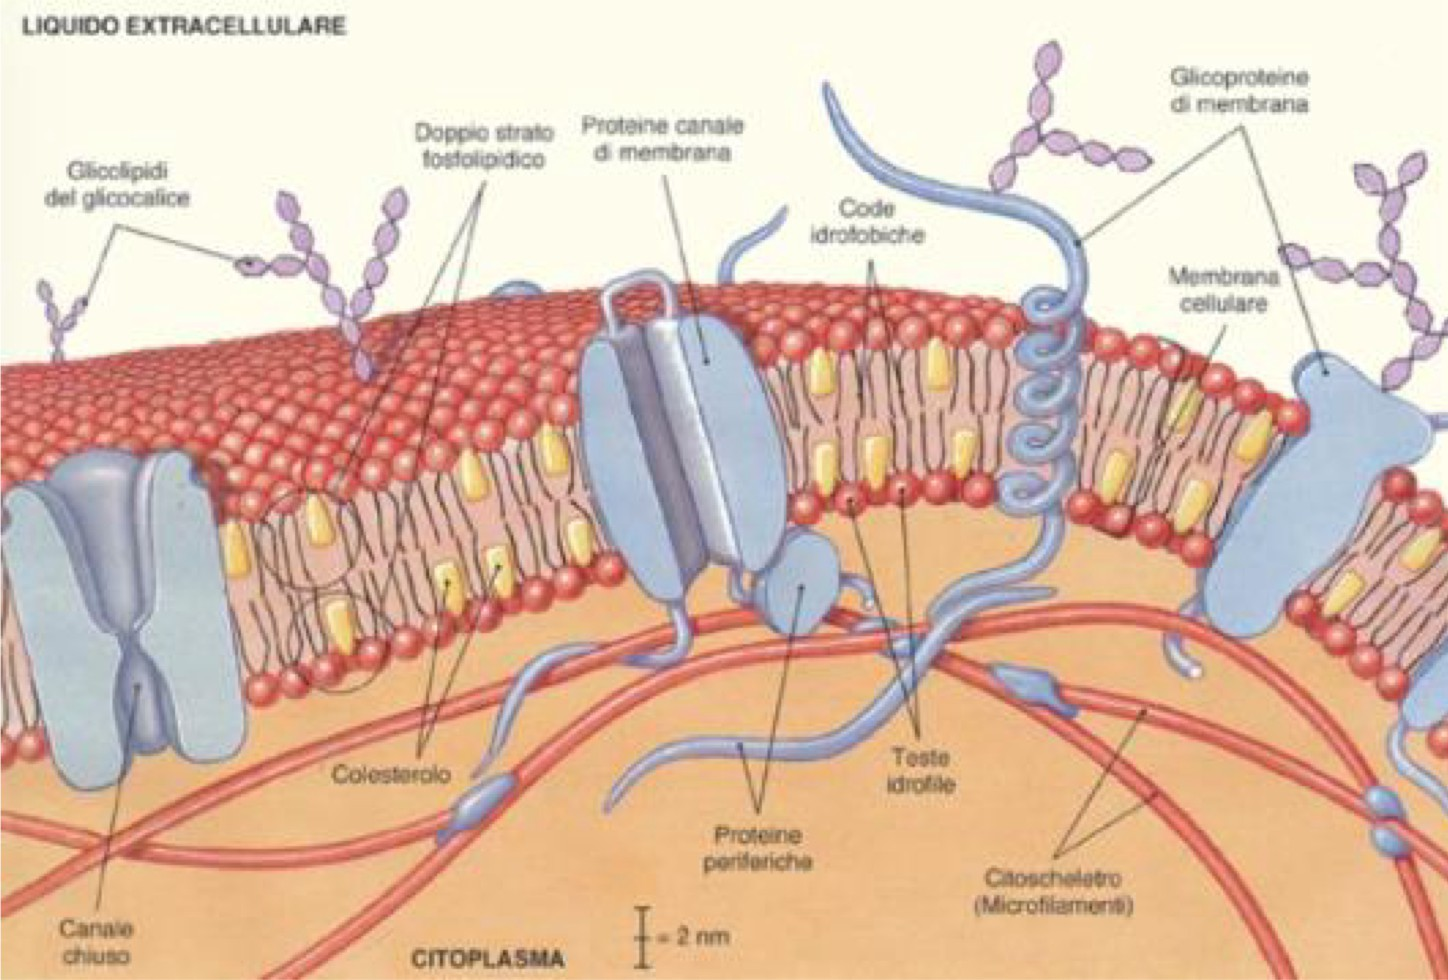
\includegraphics[width=0.80\textwidth]{images/image9.jpeg}
\end{figure}

Il cuore del funzionamento della cellula nervosa sta nella membrana cellulare: essa è ciò che distingue il neurone dalle altre cellule. Tale membrana svolge varie funzioni: tiene insieme la cellula, le dà una forma e assicura il corretto svolgimento delle funzioni precedentemente elencate. È caratterizzata dalla variazione di tre grandezze elettriche: potenziale di membrana, corrente di membrana e correnti intra extra cellulari.

La membrana è costituita da un doppio strato fosfolipidico, caratterizzato da teste fosforiche e idrofile e da code lipofile (non si collegano con l'acqua ma con i lipidi) e idrofobe, le teste si trovano esternamente mentre le code internamente. La membrana separa la parte interna della cellula (riempita di una soluzione a base acquosa, \textbf{citoplasma} o \textbf{citosol}) dall'esterno (ambiente \textbf{extracellulare}).

Ci sono delle proteine, dette proteine integrali, che attraversano la membrana da parte a parte, permettendo il passaggio controllato di sostanze; esistono delle proteine che si trovano solo sul lato esterno interno e sono dette proteine periferiche.


\subsection{Ioni coinvolti nell'attività neuronale}

I neuroni funzionano grazie al movimento di alcuni ioni (Na$^{+}$, K$^{+}$, Ca$^{2}$$^{+}$ e Cl$^{-}$) dentro e fuori la cellula. Questi ioni non sono distribuiti in modo uguale: ce ne sono di più fuori o dentro a seconda del tipo (la letteratura ci dice le concentrazioni).

Questa differenza crea due effetti:

\begin{itemize}
  \item una differenza di concentrazione (chimica),
  \item una differenza di carica elettrica (elettrica),
\end{itemize}
Insieme formano la differenza elettrochimica, che è ciò che permette al neurone di trasmettere segnali.


\subsection{Il potenziale di membrana}

Il potenziale di membrana è la differenza di potenziale tra l'interno e l'esterno della cellula, misurata con un voltmetro (elettrodo di riferimento all'esterno, esplorante all'interno). La membrana alterna due condizioni: a riposo, quando è in equilibrio, e attiva, quando varia.

A riposo, il potenziale non è nullo ma rappresenta un ``riposo attivo'', simile a una molla carica, pronto a generare risposta. Tale valore deriva dall'equilibrio tra forze elettriche e chimiche che agiscono sugli ioni (Na$^{+}$, K$^{+}$, Ca$^{2}$$^{+}$ e Cl$^{-}$).

L'equilibrio elettrochimico è dato da due forze, la differenza di concentrazione e temperatura (la forza chimica) e le forze

elettriche (ioni positivi attratti dal potenziale negativo, ioni negativi dal potenziale positivo).

L'effetto sommato di queste due forze dà origine ad un equilibrio, spiegato dall'equazione di Nernst.

\begin{figure}[htbp]
  \centering
  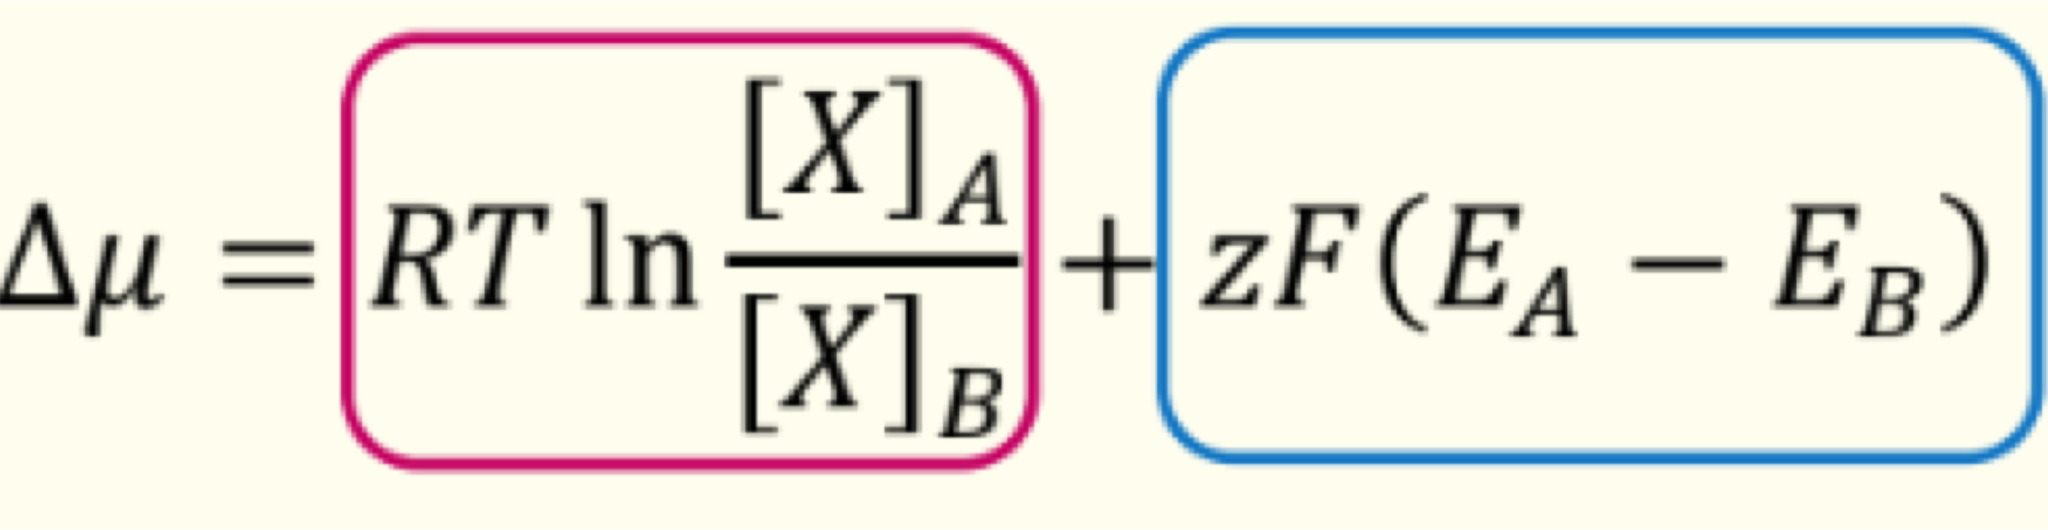
\includegraphics[width=0.80\textwidth]{images/image10.png}
\end{figure}

Il termine chimico (in rosso) scompare se le concentrazioni sono uguali, mentre il termine elettrico (in blu) dipende da z e dalla differenza di potenziale.

Le due componenti agiscono insieme: se spingono lo ione nella stessa direzione, il movimento è facilitato; se agiscono in direzioni opposte, la direzione dipende dalla loro somma. Quando le due forze si equilibrano, si raggiunge il potenziale di equilibrio, cioè il valore stabile del potenziale di membrana a riposo.


\subsection{Energie in gioco}

Il movimento degli ioni è determinato da due forze principali: il \textbf{gradiente di concentrazione }e il \textbf{potenziale elettrico}.

Gli ioni possiedono energia cinetica dovuta alla temperatura, che li fa muovere casualmente secondo il moto browniano; se c'è una differenza di concentrazione tra due regioni, si crea uno spostamento netto dalla zona più concentrata a quella meno concentrata. Questo meccanismo è proporzionale alla temperatura: più le particelle si muovono velocemente, maggiore sarà la diffusione.

La seconda forza deriva dal potenziale elettrico della membrana. Gli ioni carichi vengono spinti verso l'interno o l'esterno a seconda del segno della loro carica e della polarità del potenziale: ad esempio, un ione positivo sarà attratto verso l'interno se l'interno della cellula è più negativo, mentre un ione negativo sarà respinto verso l'esterno.

In totale, si possono avere quattro combinazioni possibili tra segno della carica e polarità del potenziale, che determinano la direzione dello spostamento. In questo caso l'energia che muove gli ioni è l'energia potenziale elettrica.

Per descrivere questi fenomeni si utilizzano costanti diverse a seconda che si consideri un singolo ione o una mole di ioni: per un singolo ione si usa la costante di Boltzmann, mentre per una mole di ioni si usa la costante universale dei gas, ottenuta moltiplicando la costante di Boltzmann per il numero di Avogadro. L'energia elettrica, invece, dipende dalla valenza dell'ione e dalla differenza di potenziale.

In sintesi, il movimento ionico è il risultato dell'interazione tra energia termica e potenziale elettrico, con direzione e intensità determinate dal gradiente di concentrazione e dal campo elettrico, e con energia fornita rispettivamente dall'energia cinetica e dall'energia potenziale elettrica.


\subsection{Equazione di Nernst}

RECAP: L'equazione di Nernst descrive il potenziale di equilibrio elettrochimico di un singolo tipo di ione attraverso una membrana. Gli ioni sono soggetti a due forze principali, tali la forza chimica e la forza elettrica. Il potenziale di membrana a cui le forze chimiche ed elettriche si bilanciano è chiamato potenziale di equilibrio, è il valore di membrana per cui uno specifico tipo di ione non si sposta più.

\begin{figure}[htbp]
  \centering
  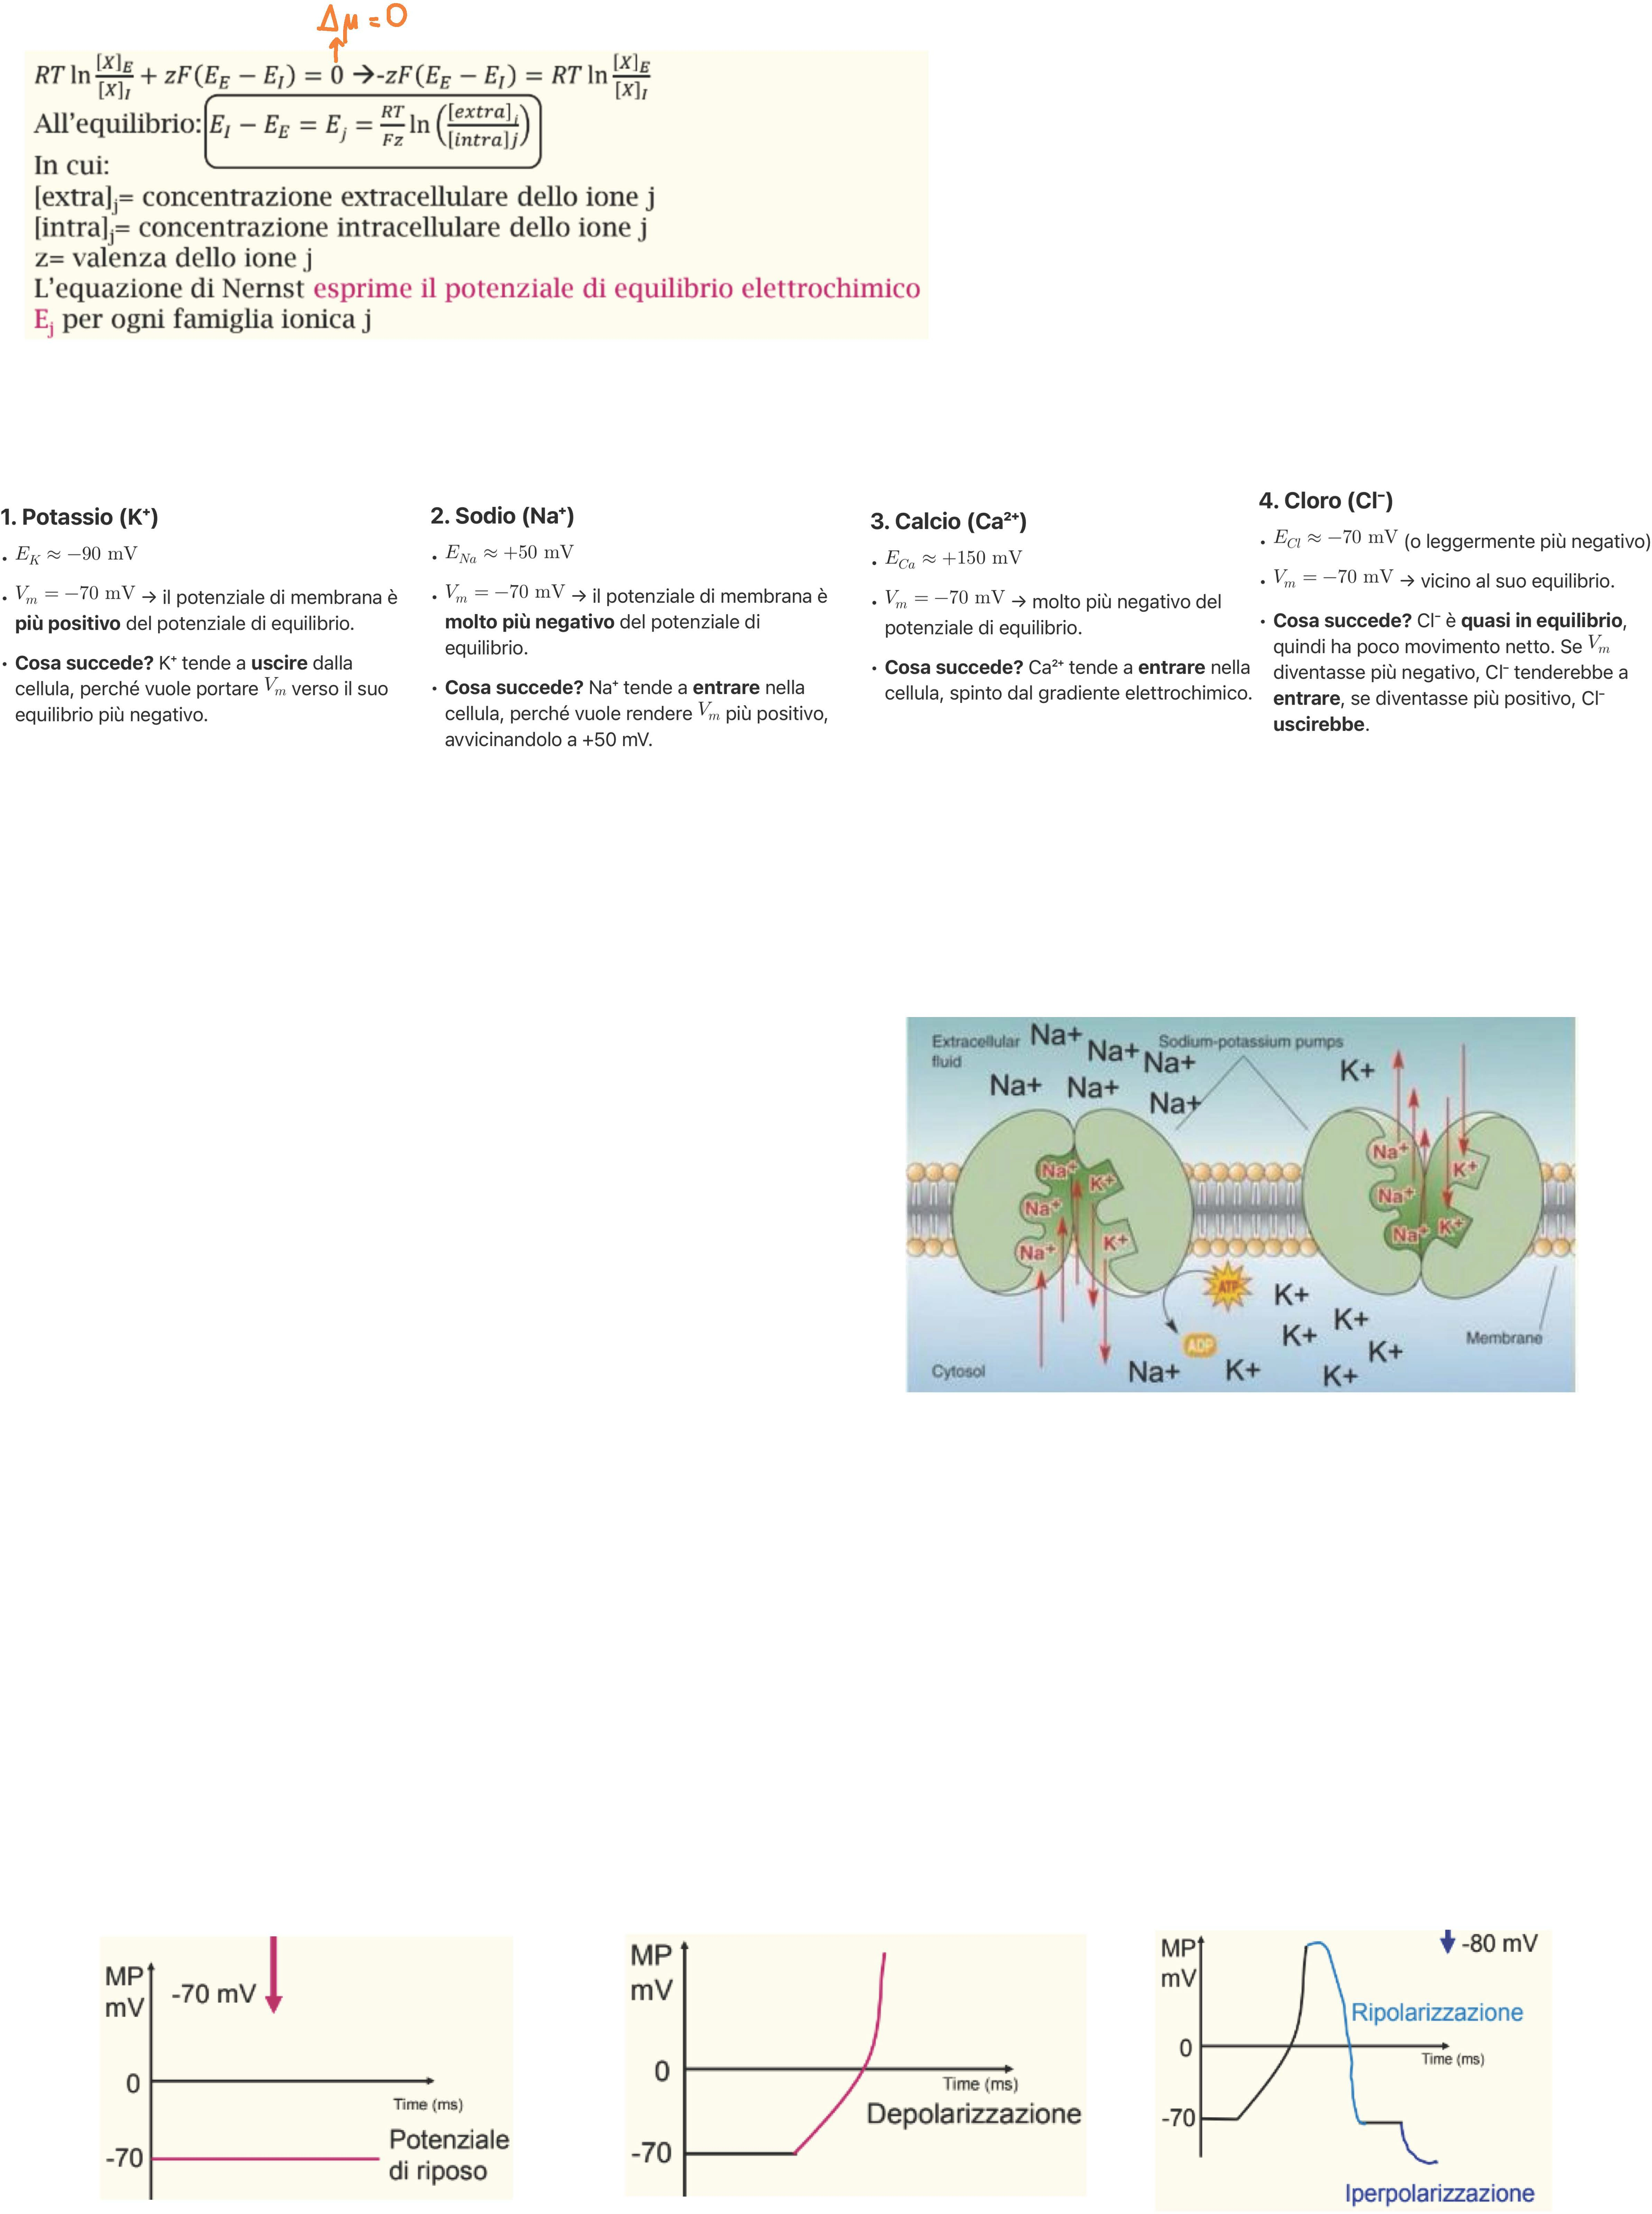
\includegraphics[width=0.80\textwidth]{images/image12.jpeg}
\end{figure}

Ora vogliamo capire qual è la condizione della membrana per la quale gli ioni non si spostano più. Per trovarlo metto a 0 il delta u, poi vado a ricavare la d.d.p. e quindi trovo il potenziale di equilibrio elettrochimico con il quale lo ione non si sposta più.

In generale, se il potenziale di equilibrio di uno ione è inferiore al potenziale di membrana, gli ioni positivi tenderanno a uscire quelli negativi ad entrare; se invece il potenziale di equilibrio è superiore al potenziale di membrana, gli ioni positivi entreranno e quelli negativi usciranno.


\subsection{Meccanismi di trasporto di membrana}

Gli spostamenti che avvengono seguendo il gradiente elettrochimico (visti ora) prendono il nome di \textbf{trasporto passivo}, in quanto lo spostamento avviene esclusivamente mediante l'energia (cinetica potenziale) fornita dagli ioni stessi.

Tuttavia esiste un altro tipo di trasporto detto \textbf{trasporto attivo}, non utilizza il gradiente elettrochimico (gli ioni si spostano contro gradiente) ma le \textbf{pompe ioniche}. L'energia usata questa volta è fornita dalla cellula ed è l'\textbf{ATP}.

Esistono diverse pompe ioniche, la più importante è la

\textbf{pompa sodio-potassio}.

La pompa sodio-potassio cambia la sua conformazione per esporre alternativamente i siti di legame verso l'interno o l'esterno della cellula. Durante il ciclo, trasporta 3 ioni sodio dall'interno verso l'esterno e 2 ioni potassio dall'esterno verso l'interno, consumando 1 molecola di ATP per ogni ciclo. Questo meccanismo non simmetrico permette di mantenere e ripristinare l'equilibrio ionico della cellula.


\subsection{Cause del potenziale di riposo}

Le quattro principali famiglie ioniche (Na$^{+}$, K$^{+}$, Cl$^{-}$, Ca$^{2}$$^{+}$) vengono continuamente spostate attraverso la membrana dai tre meccanismi visti: diffusione, forze elettriche e pompe ioniche. Nonostante questo movimento costante, il potenziale di membrana rimane stabile nel tempo, perché la risultante di tutti gli spostamenti è bilanciata.

Questo stato di equilibrio dinamico prende il nome di \textbf{potenziale di riposo}, che nei neuroni è di circa -70 mV, con l'interno della cellula più negativo rispetto all'esterno, quindi la membrana è polarizzata.

Quando si verifica una perturbazione, flussi di ioni positivi attraversano la membrana, riducendo la sua polarizzazione: questo fenomeno si chiama \textbf{depolarizzazione}. Gli ioni che provocano questo effetto sono detti \textit{ioni depolarizzanti}, e le correnti generate si chiamano \textit{correnti depolarizzanti}. Successivamente, la membrana può tornare al potenziale di riposo attraverso la \textbf{ripolarizzazione}, dovuta a \textit{ioni e correnti ripolarizzanti}. Se la membrana diventa ancora più negativa del valore di riposo, si verifica l'\textbf{iperpolarizzazione}, cioè un aumento della polarizzazione.


\subsection{Diffusione facilitata: i canali ionici}

La diffusione facilitata avviene tramite \textbf{canali ionici}, tali proteine che permettono il passaggio selettivo di specifici ioni attraverso la membrana, senza consumo di energia (\textit{passaggio selettivo di ioni in modo passivo}), poiché agiscono secondo gradiente di concentrazione.

Ogni canale è \textbf{selettivo}: ad esempio, un canale per il sodio non permette il passaggio del potassio e viceversa.

I canali possono essere sempre aperti oppure dotati di un ``cancello'' che ne regola l'apertura e la chiusura. L'apertura di questi canali può dipendere da diversi fattori:

\begin{itemize}
  \item agenti chimici (che si legano al canale direttamente o indirettamente, come nei recettori sinaptici) $\rightarrow$ canali chimico-dipendenti;
  \item variazioni del potenziale di membrana $\rightarrow$ canali voltaggio-dipendenti;
  \item stimoli fisici come luce, temperatura o pressione $\rightarrow$ canali attivati da stimoli fisici.
\end{itemize}
\textbf{Canale Na+ voltaggio-dipendente}

\begin{figure}[htbp]
  \centering
  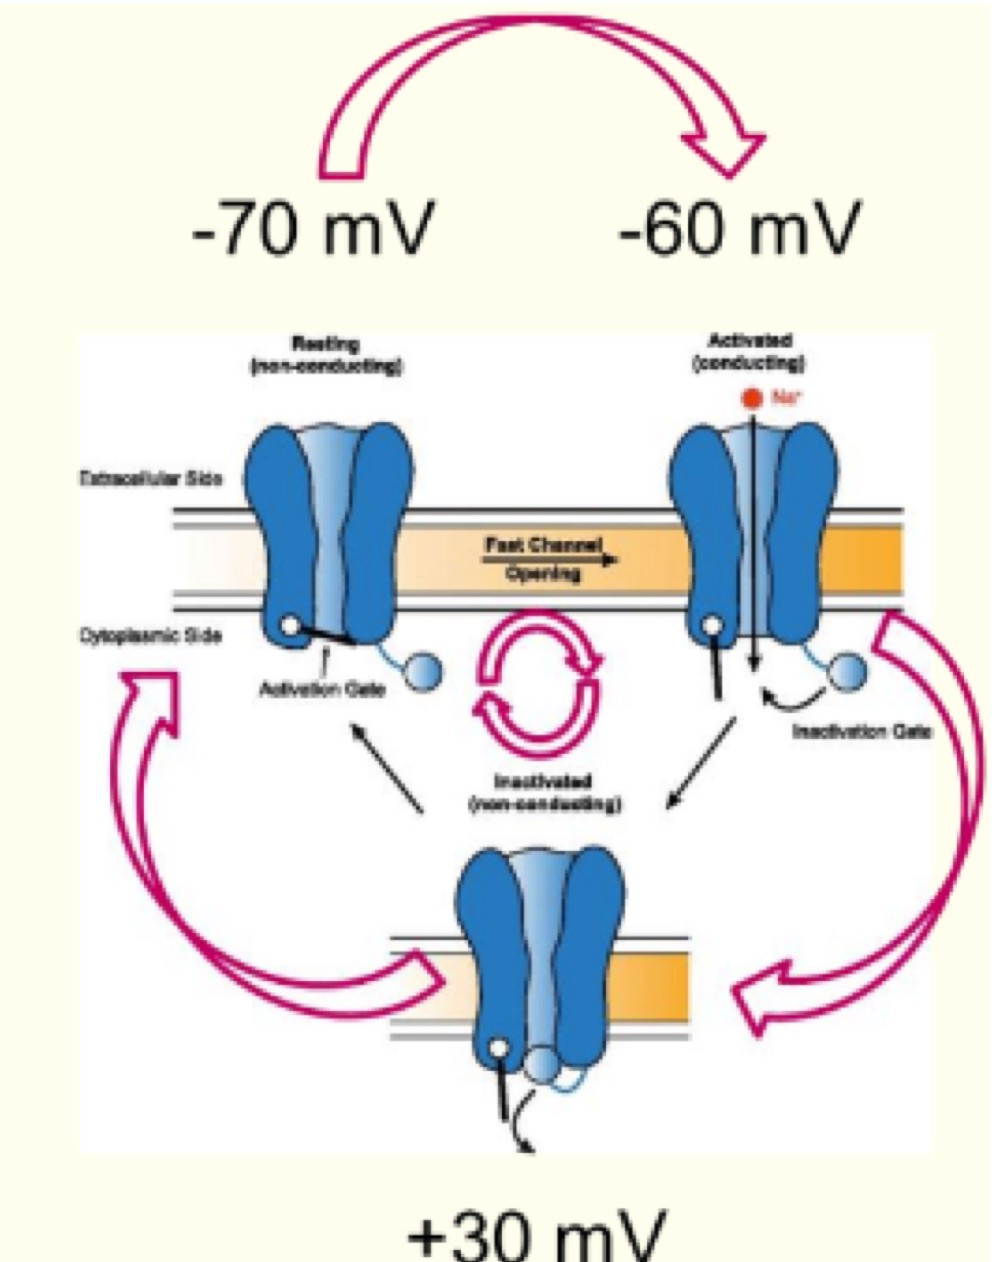
\includegraphics[width=0.80\textwidth]{images/image13.jpeg}
\end{figure}

Il canale del sodio è una proteina di membrana che può assumere tre configurazioni: chiuso, aperto e inattivo. Nello stato di chiusura, il canale non permette il passaggio di ioni ma può aprirsi; nello stato di apertura, cambia forma e lascia passare gli ioni sodio; nello stato di inattivazione, il passaggio degli ioni è nuovamente impedito, ma il canale non può riaprirsi direttamente, deve prima tornare allo stato di chiusura.

Il passaggio tra questi stati dipende dal potenziale di membrana, che determina soglie specifiche di attivazione e inattivazione:

\begin{itemize}
  \item A --70 mV (potenziale di riposo), il canale è chiuso;
  \item Se il potenziale si depolarizza e raggiunge circa --60 mV, il canale si apre, permettendo l'ingresso di ioni sodio dall'esterno verso l'interno, secondo gradiente elettrochimico;
  \item L'ingresso di sodio aumenta la depolarizzazione fino a circa +30 mV, momento in cui il canale si inattiva e il flusso ionico si interrompe.
\end{itemize}
\begin{figure}[htbp]
  \centering
  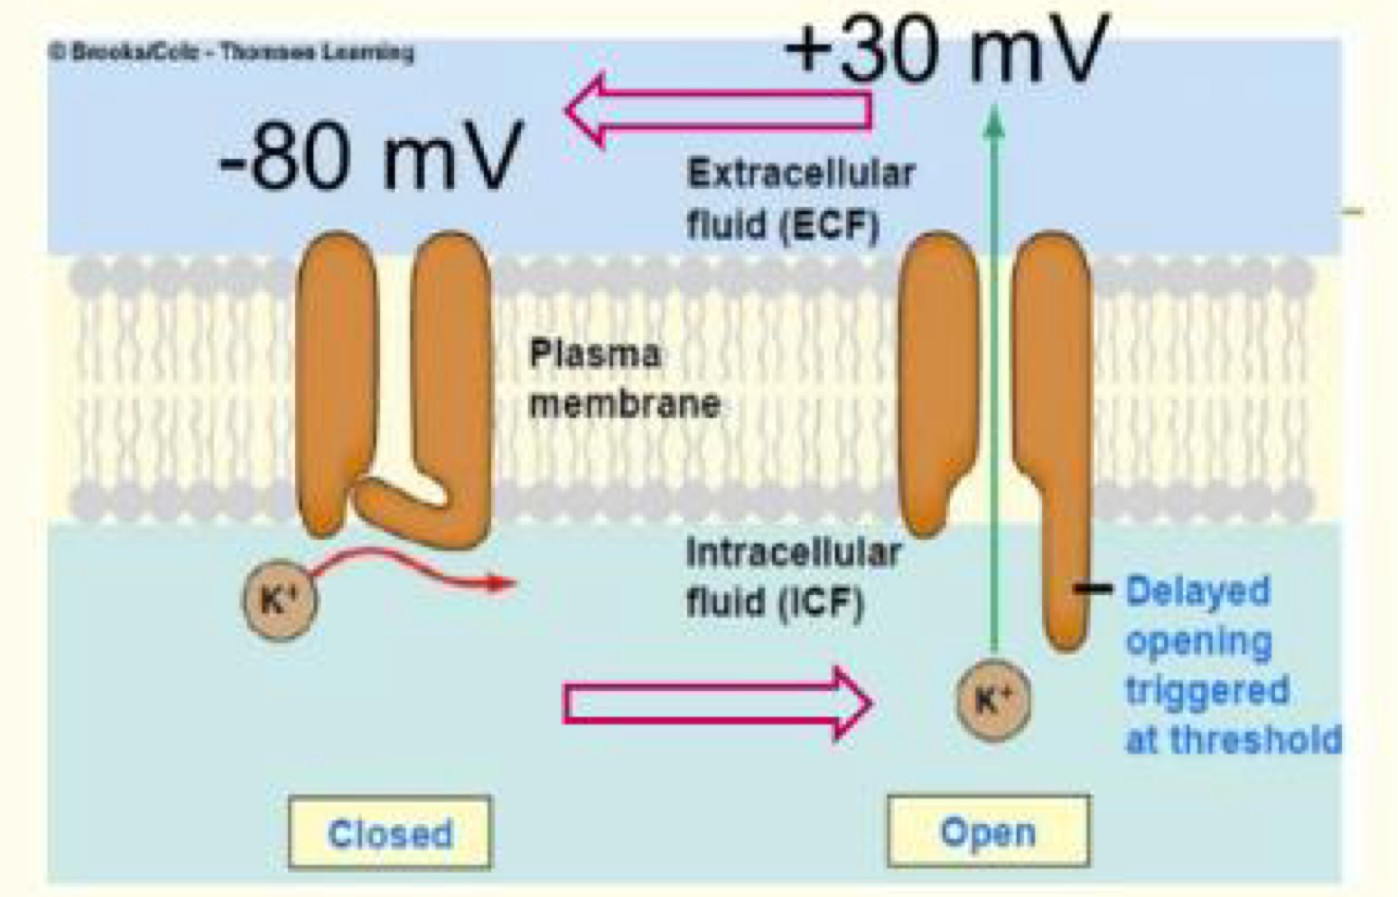
\includegraphics[width=0.80\textwidth]{images/image14.jpeg}
\end{figure}

Quando la membrana si ripolarizza (torna negativa), il canale non si riapre subito, ma passa dallo stato inattivo a quello chiuso a --70 mV, pronto a riattivarsi in seguito. Lo stato di inattività ha la funzione di impedire una riapertura troppo precoce del canale, garantendo che la sequenza di apertura e chiusura avvenga in modo ordinato e controllato durante il potenziale d'azione.

\textbf{Canale K+ voltaggio-dipendente}

Il canale del potassio (K$^{+}$) a voltaggio-dipendente è un canale a cancello elettricamente controllato, che cambia configurazione in base al potenziale di membrana. Può trovarsi solo in due stati: \textbf{aperto }o \textbf{chiuso}, con due soglie precise: +30 mV per l'apertura e --80 mV per la chiusura. A riposo (--70 mV)

il canale è chiuso. Quando avviene una depolarizzazione, il canale rimane

chiuso fino al raggiungimento di +30 mV, valore in cui il canale del sodio si inattiva e quello del potassio si apre, permettendo il passaggio degli ioni K$^{+}$. Il canale del potassio quindi agisce in senso opposto a quello del sodio, contribuendo al ritorno del potenziale a valori negativi.

\begin{figure}[htbp]
  \centering
  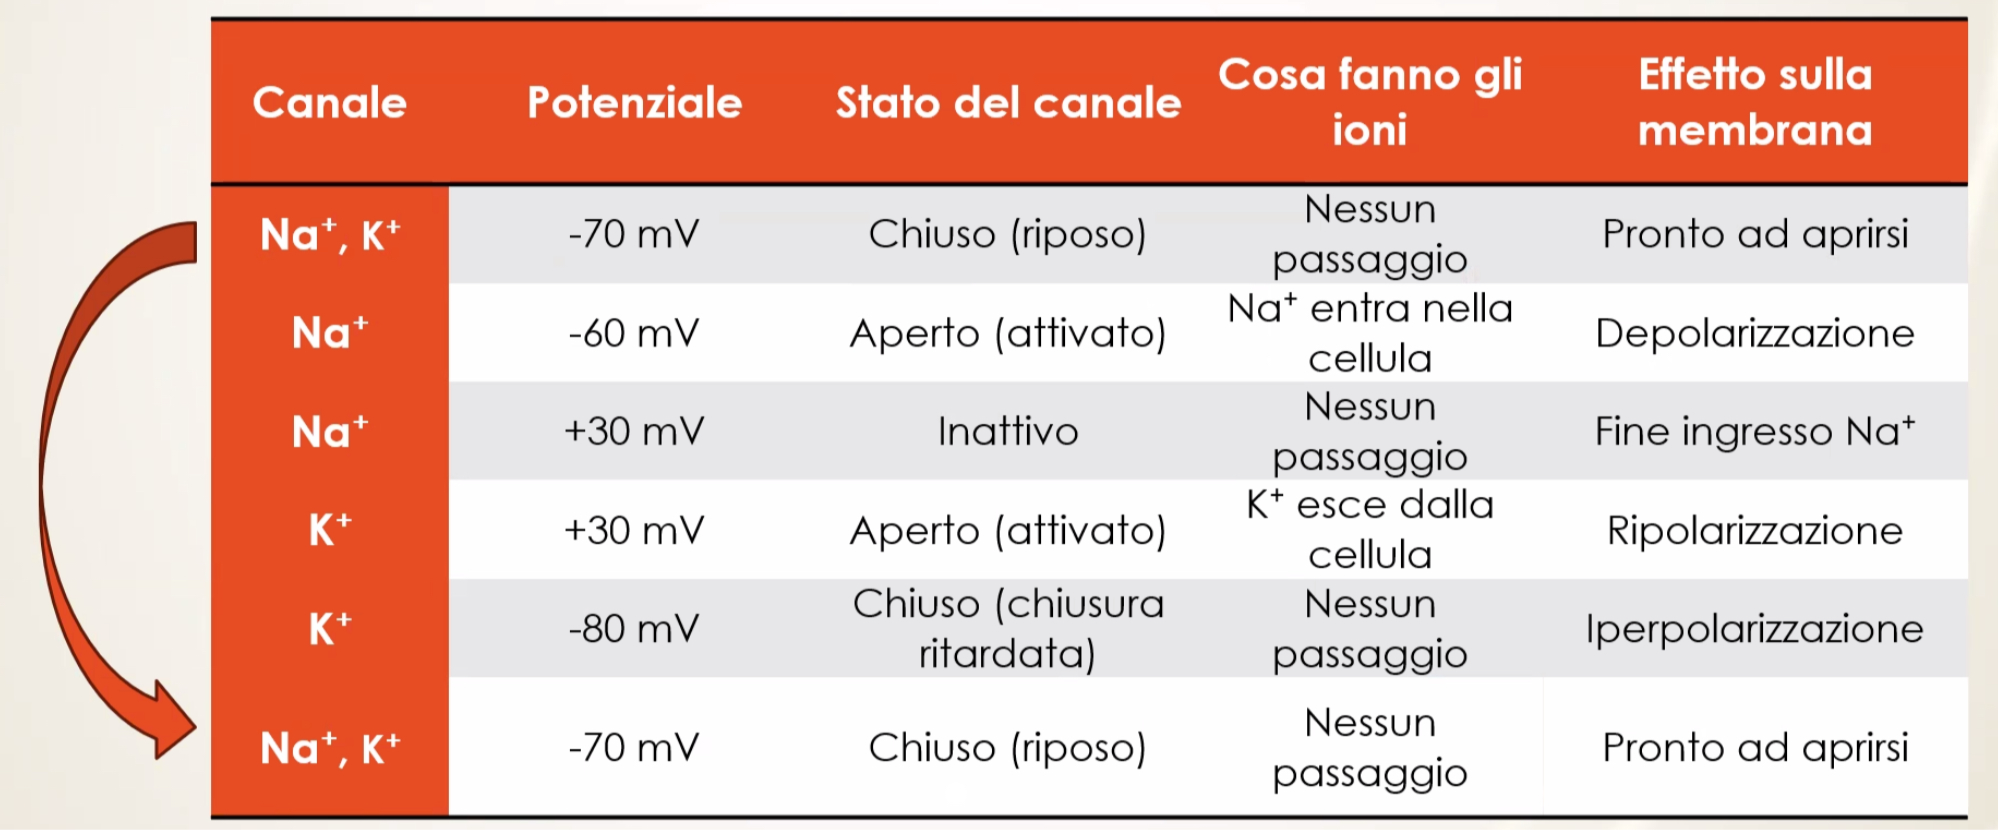
\includegraphics[width=0.80\textwidth]{images/image15.png}
\end{figure}

La soglia di chiusura è --80 mV, inferiore al potenziale di riposo (--70 mV), perciò è necessaria un'iperpolarizzazione per richiudere il canale. Poiché il potenziale di equilibrio del K$^{+}$ è --90 mV, gli ioni potassio continuano a uscire anche oltre i --80 mV, spingendo la membrana verso l'iperpolarizzazione e favorendo la chiusura del canale.


\clearpage
\textbf{1b. Generazione e propagazione del potenziale d'azione, potenziali graduati}


\subsection{Il potenziale d'azione}

Il potenziale d'azione è una variazione del potenziale di membrana (da qui ``potenziale'') osservabile in punti specifici della cellula, che permette alla cellula di inviare segnali ad altre cellule, entrando così ``in azione'' (da qui ``d'azione'').

Non tutte le cellule lo generano: solo le \textbf{cellule eccitabili }(nervose, muscolari striate e cardiache).

Ha una forma sempre identica, con ampiezza, durata e andamento costanti, per cui l'informazione non dipende da queste caratteristiche.

Funziona secondo il principio del ``tutto o nulla'': o non avviene, oppure, se si genera, è sempre uguale, come un segnale binario (0 o 1).

Si verifica quando la membrana si depolarizza fino a circa -60 mV, indicando che è regolato da un meccanismo a soglia.


\subsection{Generazione del potenziale d'azione}

\begin{figure}[htbp]
  \centering
  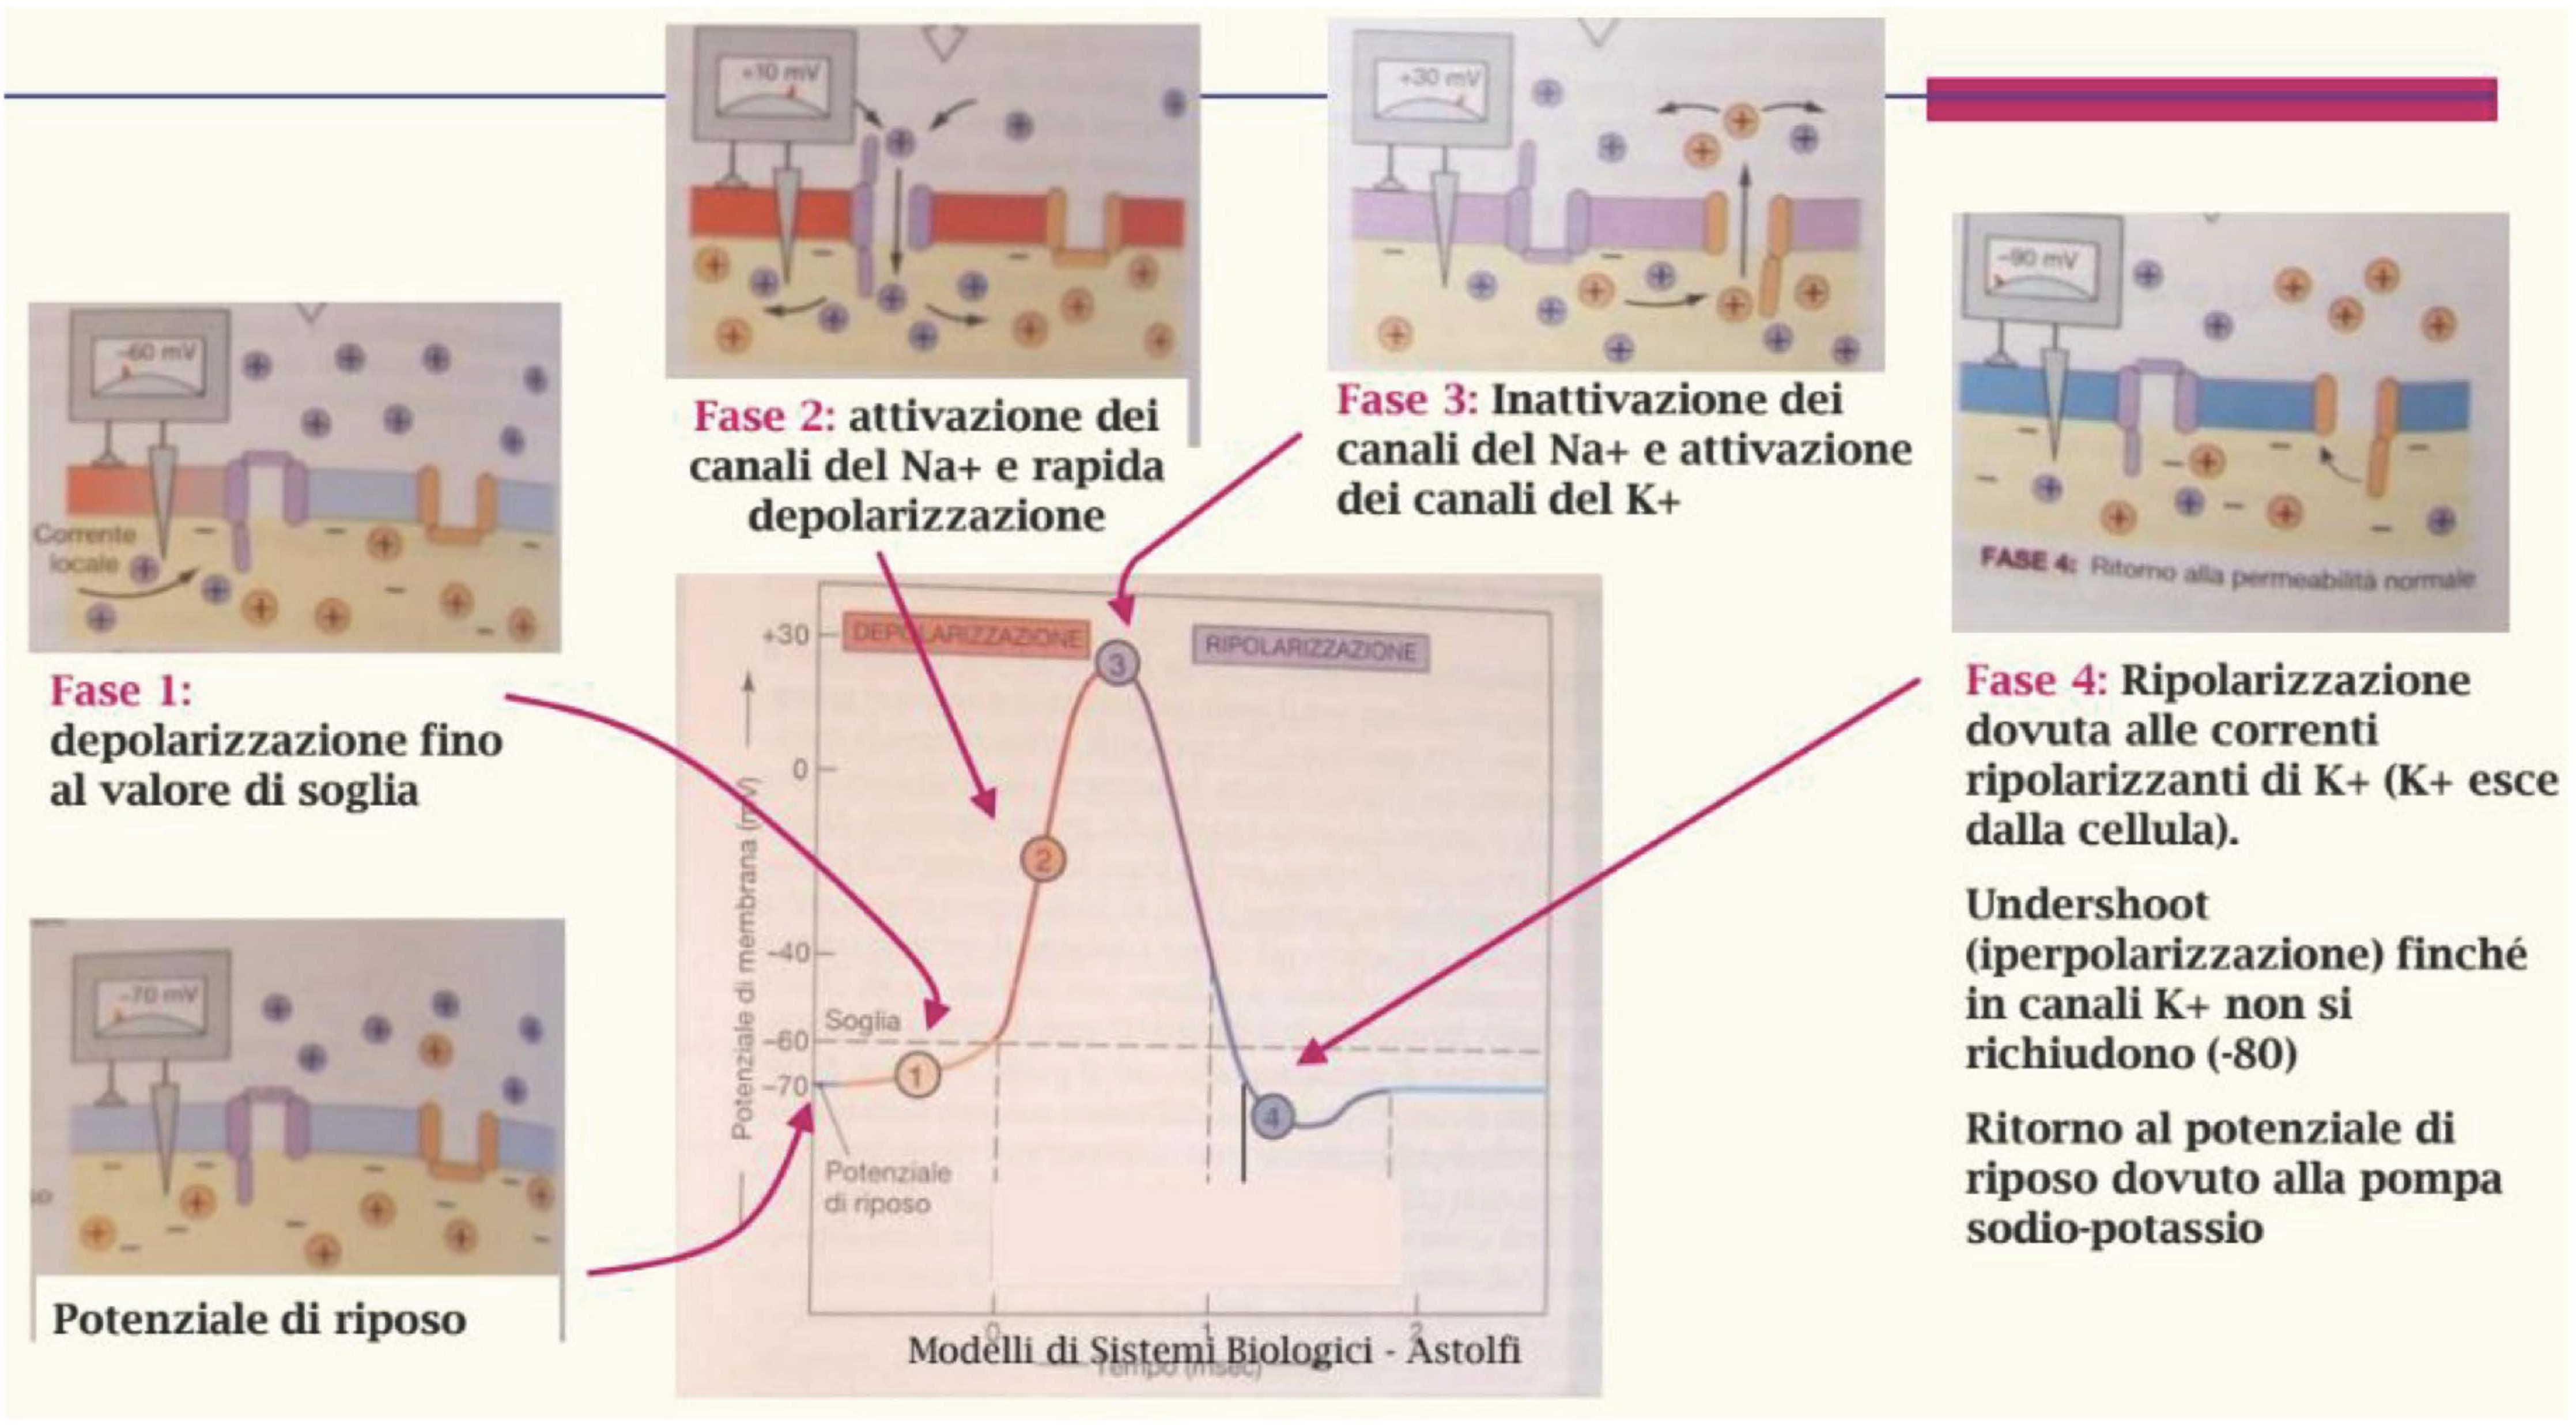
\includegraphics[width=0.80\textwidth]{images/image17.jpeg}
\end{figure}

In figura è rappresentato l'andamento del potenziale d'azione. Sull'asse delle ascisse si ha il tempo in ms, mentre sull'asse delle ordinate si ha il potenziale di membrana, espresso in mV.

La generazione del potenziale d'azione segue un andamento preciso nel tempo:

\begin{itemize}
  \item \textbf{Riposo}: la membrana è a -70 mV, con canali di sodio e potassio chiusi. Piccole variazioni intorno al potenziale di riposo possono avvenire, ma il meccanismo importante parte solo quando si raggiunge la soglia di -60 mV.
  \item \textbf{fase 1- Soglia di attivazione }(-60 mV): se la depolarizzazione raggiunge questa soglia, si apre il canale del sodio.
  \item \textbf{fase 2 - Depolarizzazione rapida}: gli ioni sodio entrano nella cellula, causando un rapido aumento del potenziale fino a circa +30 mV. Il canale del sodio si inattiva a questo punto, interrompendo il flusso.
  \item \textbf{fase 3 - Ripolarizzazione}: si aprono i canali del potassio; il potassio esce dalla cellula, riportando la membrana verso il potenziale di riposo (-70 mV). I canali del potassio si chiudono a -80 mV, causando un'iperpolarizzazione temporanea.
  \item \textbf{fase 4 - Ripristino dell'equilibrio}: le pompe sodio-potassio riportano gli ioni nelle loro posizioni iniziali, ripristinando completamente il potenziale di membrana.
\end{itemize}
Indipendentemente dal percorso iniziale, una volta raggiunta la soglia di -60 mV, il meccanismo è sempre lo stesso: apertura e chiusura dei canali e delle pompe sono costanti, così come il numero di ioni coinvolti.


\subsection{Refrattarietà assoluta}

Quando la membrana parte dal potenziale di riposo (-70 mV) e raggiunge la soglia, si apre il canale del sodio, che permette agli ioni sodio di entrare e avviare il potenziale d'azione. Poco dopo, però, questo canale diventa inattivo:

\begin{itemize}
  \item Quando è aperto, il sodio può passare normalmente;
  \item Quando è inattivo, il canale non può più aprirsi, nemmeno se lo stimolo sulla
  \item membrana diventa molto forte.
\end{itemize}
Questo significa che durante questo intervallo (viola nell'immagine) non può essere generato nessun nuovo potenziale d'azione.

Questo periodo prende il nome di \textbf{refrattarietà assoluta}: la membrana è completamente refrattaria, cioè oppone resistenza totale alla generazione di un nuovo potenziale d'azione.

In pratica, la refrattarietà assoluta dipende solo dai canali del sodio e non ammette eccezioni: finché i canali sono inattivi, il potenziale d'azione non può ricominciare. Termina quando i canali Na+ si chiudono (-70mV).


\subsection{Refrattarietà relativa}

La refrattarietà relativa inizia subito dopo la refrattarietà assoluta, quando i canali del sodio, che prima erano inattivi, si chiudono di nuovo intorno a -70 mV.

In questo momento la membrana non è ancora al potenziale di riposo perché i canali del potassio sono ancora aperti, causando una iperpolarizzazione.

I canali del sodio sono però pronti a riaprirsi, quindi è possibile generare un nuovo potenziale d'azione, ma serve uno stimolo più forte del normale, superiore ai 10 mV necessari a raggiungere la soglia di -60 mV.

Questo periodo prende il nome di \textbf{refrattarietà relativa}: la membrana non

impedisce completamente un nuovo potenziale d'azione, ma rende la sua generazione più difficile.

A differenza della refrattarietà assoluta, che dipende dai canali del sodio, quella relativa dipende dai canali del potassio ancora aperti. Termina quando i canali K+ si chiudono (-80mV).


\subsection{Sequenze di potenziale d'azione}

La cellula, in tempi brevissimi (1-2 ms), valuta continuamente se generare nuovi potenziali d'azione. La linea azzurra indica il potenziale di riposo, mentre la linea rossa rappresenta la soglia di attivazione.

Non tutte le variazioni del potenziale di membrana raggiungono la soglia: quelle più piccole, che non provocano un potenziale d'azione, si chiamano potenziali graduati. Questi sono meno ampi e più lunghi dei potenziali d'azione veri e propri.

\begin{figure}[htbp]
  \centering
  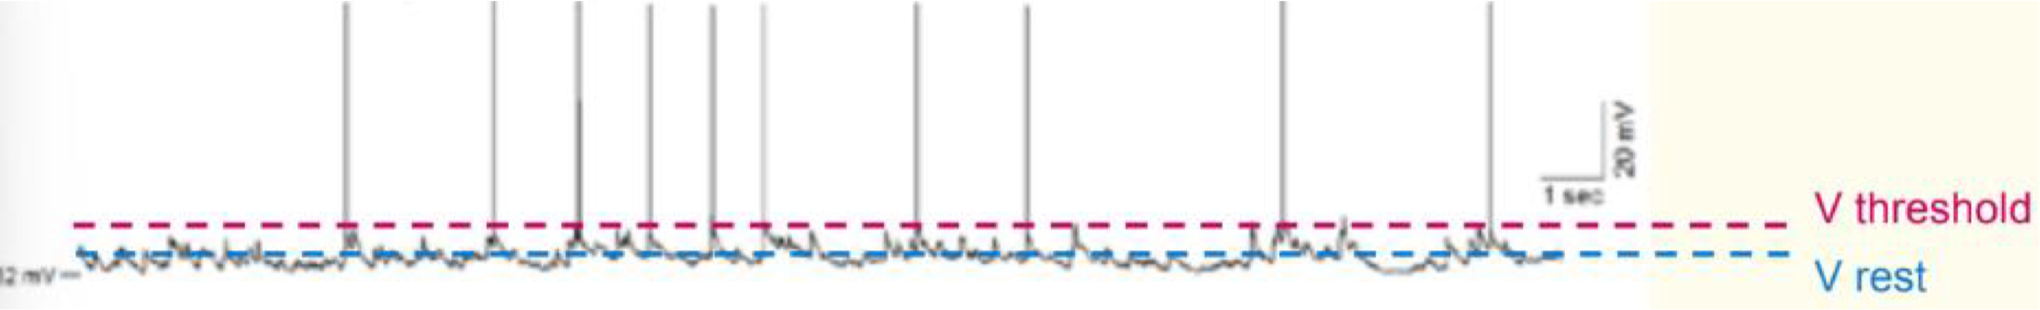
\includegraphics[width=0.80\textwidth]{images/image20.png}
\end{figure}

I potenziali d'azione, invece, si generano solo quando la perturbazione della membrana supera la soglia. Essendo tutti identici per ampiezza, forma e durata, l'informazione non sta nel singolo potenziale, ma nella sequenza con cui essi si susseguono. In altre parole, ciò che conta è quando avviene ogni potenziale d'azione e quanto spazio temporale c'è tra due segnali consecutivi, perché da questo dipende la risposta della cellula.

Brevissima durata, ampiezza elevata: simile a uno \textbf{spike }(delta di Dirac).

L'informazione non è contenuta nella forma.


\section{1b. Propagazione del potenziale d'azione}

Il potenziale d'azione può essere registrato in diverse parti della cellula, perché i canali ionici sono presenti sul soma, sui dendriti, ma soprattutto nel cono d'emergenza dell'assone e lungo l'assone stesso. Di conseguenza, è più probabile che il potenziale d'azione si generi nel cono d'emergenza.

Le informazioni ricevute dai dendriti vengono integrate dalla cellula e trasformate in una perturbazione che arriva al cono d'emergenza, dove si genera il potenziale d'azione, che viene poi propagato lungo l'assone.

La propagazione può avvenire in due modi, a seconda della struttura dell'assone:

\begin{itemize}
  \item \textbf{Continua}, nelle fibre amieliniche;
  \item \textbf{Saltatoria}, nelle fibre mielinizzate.
\end{itemize}
\begin{figure}[htbp]
  \centering
  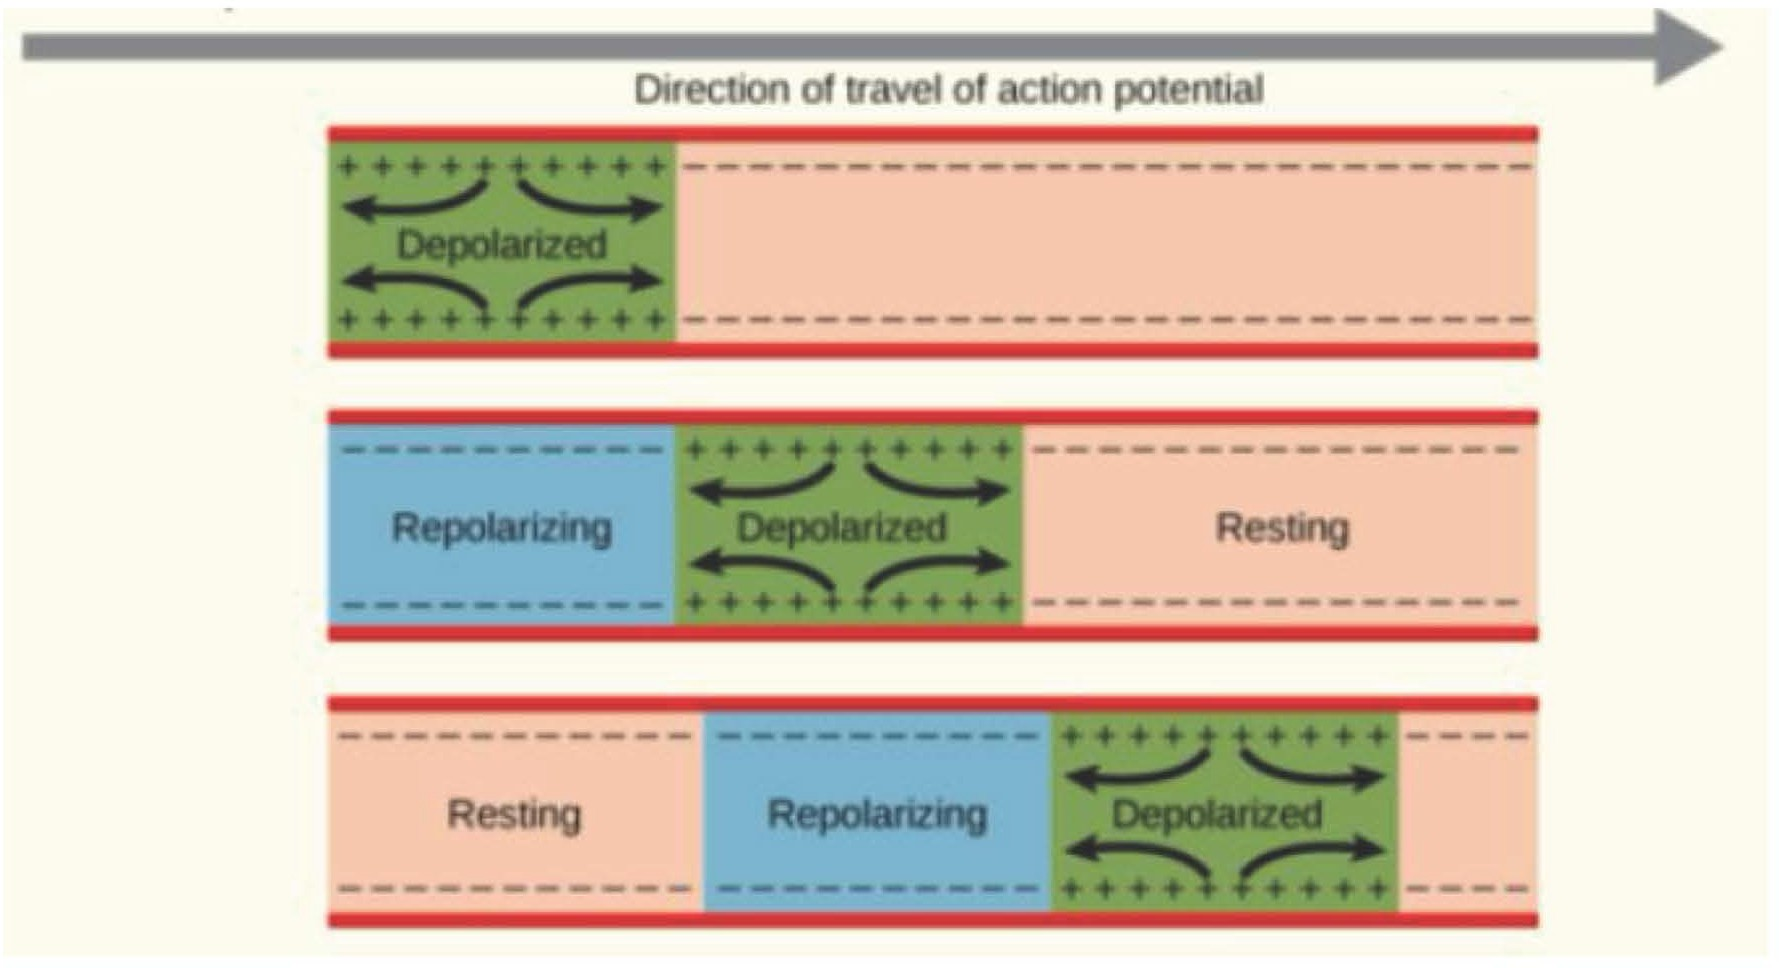
\includegraphics[width=0.80\textwidth]{images/image21.jpeg}
\end{figure}

La propagazione continua

Le correnti intracellulari hanno un corrispettivo extracellulare uguale e opposto. Per comprenderle è necessario introdurre una dimensione spaziale: se in un punto della membrana si verifica un potenziale d'azione, nelle zone circostanti la membrana è ancora a riposo, con prevalenza di cariche negative all'interno e positive all'esterno; localmente, invece, avviene un'inversione.

Come in una soluzione acquosa in cui si aggiunge una goccia ricca di ioni positivi, questi diffondono nell'ambiente intracellulare (e quelli esterni fanno lo

stesso, ma con segno opposto). La variazione si propaga quindi tramite correnti intra- ed extracellulari.

Al riposo si ha prevalenza di cariche negative interne e positive esterne. Con il potenziale d'azione compare un'inversione e le cariche positive si muovono seguendo il gradiente elettrochimico verso zone a potenziale minore, in tutte le direzioni, poiché le forze di diffusione non hanno direzione preferenziale. Le cariche raggiungono zone dove la membrana è all'equilibrio; esternamente avviene l'opposto. Tale spostamento, secondo gradiente, propaga la perturbazione.

La depolarizzazione si trasmette quindi alle zone adiacenti della membrana. Le regioni più influenzate sono quelle più vicine al punto perturbato; l'effetto si riduce con la distanza fino a scomparire.

Questo meccanismo si chiama propagazione passiva (non va confusa con il trasporto passivo). Non riguarda solo il potenziale d'azione, ma tutte le perturbazioni: è non direzionata, dipende dalla distanza e si attenua rapidamente.

Nel caso del potenziale d'azione, la perturbazione è molto intensa: se parte da 100 mV, nelle zone vicine si genera una depolarizzazione ancora forte, sempre <100 mV ma >10 mV.

Il fatto che il potenziale si generi in un punto implica che poco dopo si genererà in una zona circostante: il nuovo potenziale d'azione si propaga passivamente, ci si sposta di un altro tratto, e si ripete finché ci sono canali ionici pronti ad aprirsi.

Nella cellula questo avviene nell'assone, una struttura lunga e stretta circondata da membrana con canali voltaggio-dipendenti per Na$^{+}$ e K$^{+}$.

Il potenziale d'azione si genera nel cono d'emergenza e poi si trasmette lungo l'assone tramite propagazione passiva, con

generazione ripetuta di nuovi potenziali d'azione. Questo processo si chiama conduzione attiva e richiede molta energia. È complesso e lento.

La propagazione passiva è adirezionale, poiché basata sulla diffusione. Tuttavia, il potenziale d'azione è unidirezionale, propagando dalla cellula verso l'esterno (direzione centrifuga).

Ciò avviene perché anteriormente la membrana è a riposo e può generare un nuovo potenziale, mentre posteriormente si trova in stato refrattario.

La refrattarietà assoluta rende unidirezionale la propagazione: se non ci fosse, il potenziale d'azione andrebbe avanti e indietro nell'assone. L'unidirezionalità dipende quindi dall'inattivazione dei canali del sodio.

La propagazione continua è molto lenta, con velocità media di 1 m/s. Le vie dolorose sono vie lente e utilizzano questo meccanismo.


\subsection{La propagazione saltatoria}

La propagazione saltatoria è un diverso tipo di propagazione del potenziale che si basa su una diversa struttura dell'assone.

Rispetto all'assone ``nudo'' della conduzione continua, qui intervengono le cellule di Schwann, che avvolgono l'assone in più strati formando una guaina mielinica, simile a un nastro isolante.

Questa guaina isola l'interno dall'esterno e impedisce il passaggio di sostanze.

La mielina non ricopre tutta la lunghezza dell'assone: esistono delle interruzioni chiamate nodi di Ranvier, dove la membrana è esposta e sono presenti canali del sodio e del potassio

voltaggio-dipendenti.

La propagazione procede così: si genera la perturbazione, si produce una forte depolarizzazione, segue una breve e rapida propagazione passiva, e poi si genera un potenziale d'azione, che è

sempre uguale. L'assone rivestito si chiama assone mielinizzato; gruppi di assoni mielinizzati costituiscono le fibre nervose. Nel segmento mielinizzato la depolarizzazione si propaga passivamente, ma non può generare nuovi potenziali d'azione perché non c'è comunicazione tra interno ed esterno (la guaina isola).

Quindi in quel tratto non possono attivarsi i canali: le correnti scorrono passivamente fino al nodo successivo.

Al nodo successivo, se la distanza tra i nodi è adeguata, la perturbazione, pur attenuandosi lungo il tratto mielinizzato, arriva ancora con un'ampiezza di almeno 10 mV nella direzione della

depolarizzazione, sufficiente a generare un nuovo potenziale d'azione. La distanza tra i nodi è ottimizzata per questo. I vantaggi sono:

\begin{itemize}
  \item generazione di potenziali solo nei nodi e non lungo tutto l'assone
  \item maggiore efficienza
  \item Velocità molto elevata $\rightarrow$ circa 120 m/s
\end{itemize}
Le vie motorie sono mielinizzate, mentre quelle dolorifiche no.

Si parla di conduzione saltatoria perché il potenziale d'azione sembra comparire, sparire e poi ricomparire ai nodi, come se ``saltasse'' da un nodo all'altro.

\textbf{CAP.1 RICHIAMI DI ELETTROFISIOLOGIA CELLULARECAP.1 RICHIAMI DI ELETTROFISIOLOGIA CELLULARE1c. La trasmissione sinaptica e l'integrazione dell'informazione da parte della cellula nervosa}

\section{1c. La trasmissione sinaptica e l\'integrazione dell\'informazione}

La trasmissione dell'informazione avviene sempre tra due cellule: una cellula \textbf{inviante }(che può essere un neurone o uno stimolo esterno) e una cellula \textbf{ricevente}. L'informazione viene trasmessa sotto forma di \textbf{potenziale d'azione}, ossia una depolarizzazione intensa del potenziale di membrana, che viaggia lungo l'assone fino a raggiungere altre cellule.

Questo processo prende il nome di \textbf{trasmissione sinaptica }e avviene attraverso le sinapsi, che rappresentano le strutture fisiche responsabili del passaggio dell'informazione da una cellula all'altra.

Le cellule che ricevono informazioni possiedono dendriti, siti specifici organizzati in una struttura ramificata chiamata albero dendritico. La forma dell'albero dendritico può variare: esistono cellule con strutture diverse, ma tutte condividono la struttura base composta da: soma e ramificazioni com forma e distribuzione differenti. Le informazioni inviate dalla cellula si presentano come un unico segnale che cambia nel tempo, e possono essere molteplici e di origine diversa. Essa inoltre è un segnale elettrico, cioè una variazione di una grandezza elettrica, che viaggia tra le cellule creando una connessione elettrica per trasferire l'informazione.

L'informazione ha la forma di un segnale elettrico, cioè una variazione di una grandezza elettrica che viaggia da una cellula all'altra creando una connessione utile al trasferimento. Questo fenomeno in natura prende il nome di sinapsi elettrica, anche se non è il meccanismo più comune. In ogni sinapsi ci sono due cellule: la pre-sinaptica, che invia l'informazione, e la post-sinaptica, che la riceve. I ruoli non sono interscambiabili. I principali vantaggi della sinapsi elettrica sono la velocità elevata e la sincronizzazione tra cellule.

La cellula pre-sinaptica invia il segnale sotto forma di potenziale d'azione (impulso nervoso). In realtà arriva una sequenza di potenziali d'azione, ma consideriamo un singolo impulso: esso percorre l'assone fino al bottone sinaptico, dove incontra la cellula post-sinaptica. Quest'ultima riceve l'informazione tramite il proprio albero dendritico. Nelle sinapsi elettriche le membrane pre e post-sinaptiche sono collegate da gap junctions, proteine che ancorano le due membrane e mettono in continuità i liquidi intracellulari. I loro pori, sempre aperti, permettono il passaggio libero degli ioni tra le cellule. Quando arriva l'impulso nervoso, si verifica una depolarizzazione: le cariche positive passano alla cellula post-sinaptica, che si depolarizza a sua volta. In questo modo il segnale viene trasmesso mantenendo la sua natura elettrica.

Questo meccanismo, però, ha un limite: poiché il segnale è sempre una depolarizzazione, l'effetto sulla membrana post-sinaptica è sempre lo stesso, positivo. Non può mai cambiare segno. Per questo motivo la sinapsi elettrica, pur essendo semplice, veloce e sincronizzata, risulta poco comune.

\begin{figure}[htbp]
  \centering
  
\includegraphics[width=0.80\textwidth]{images/image23.png}
\end{figure}

Si tratta di un meccanismo molto più diffuso e complesso, ma con enormi vantaggi. In questa sinapsi le due cellule \textbf{non }si toccano, non esiste una continuità fisica, ma uno spazio detto \textbf{fessura sinaptica}. L'informazione elettrica che arriva sulla cellula pre-sinaptica cambia natura: diventa un segnale chimico per attraversare la fessura e raggiungere la cellula post-sinaptica. Il messaggero è quindi di tipo chimico, e il segnale passa da elettrico a chimico, per poi tornare di nuovo elettrico. La trasformazione è mediata dai neurotrasmettitori.

\begin{figure}[htbp]
  \centering
  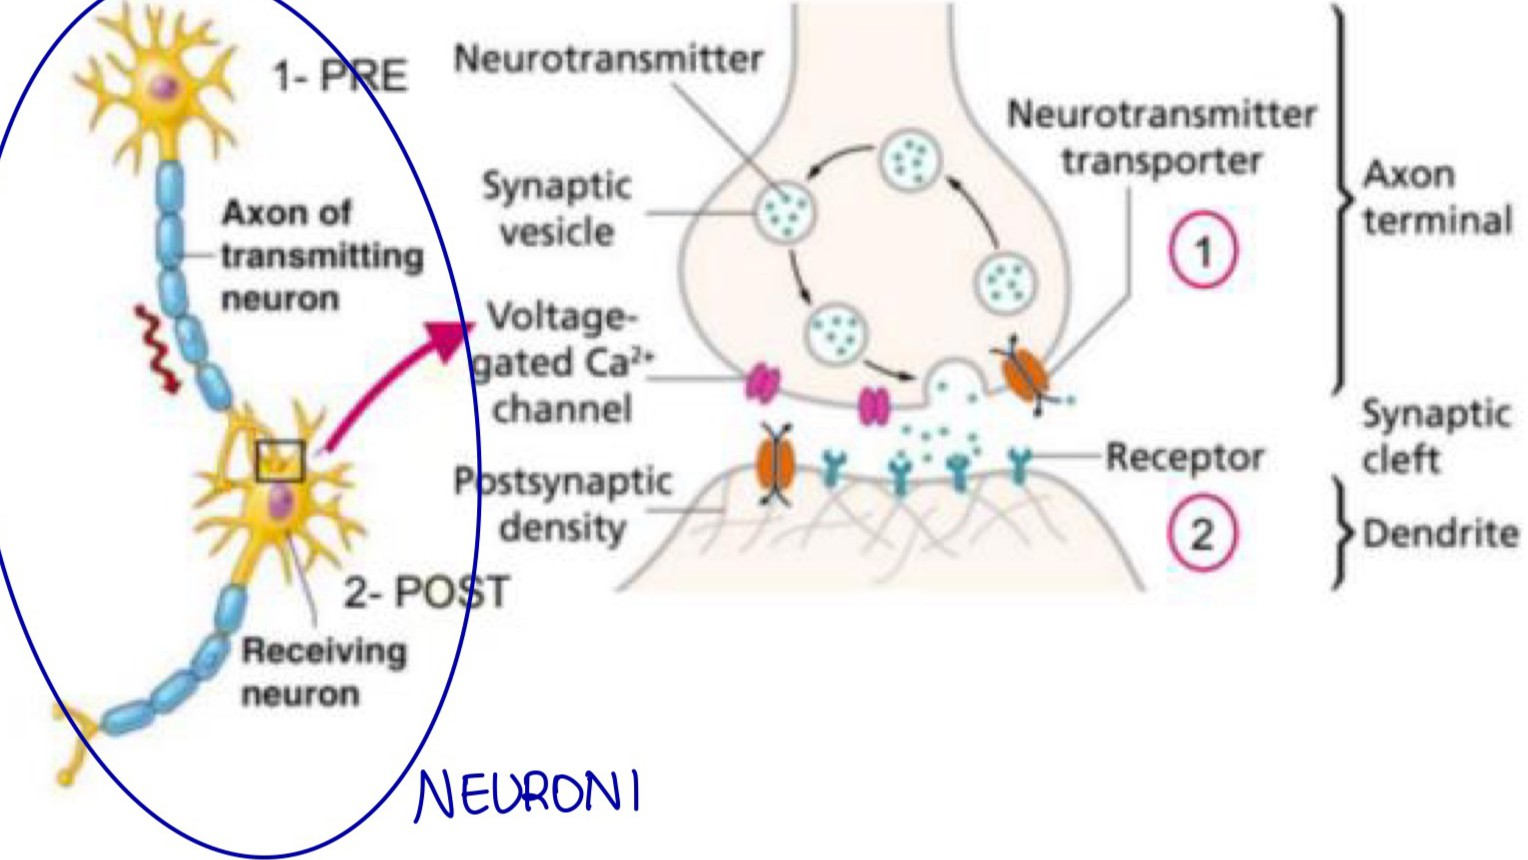
\includegraphics[width=0.80\textwidth]{images/image24.jpeg}
\end{figure}

Nell'immagine si osservano due neuroni che fanno sinapsi, l'arrivo del potenziale d'azione lungo l'assone mielinizzato e l'ingrandimento della fessura sinaptica tra il bottone sinaptico del neurone pre-sinaptico e l'albero dendritico del neurone post-sinaptico. Perché avvenga una sinapsi chimica sono necessarie strutture specifiche. Nella cellula pre-sinaptica, lungo la membrana, ci sono canali voltaggio-dipendenti per lo ione calcio. Quando arriva il potenziale d'azione, i canali si aprono: il calcio, presente soprattutto all'esterno, entra nella cellula secondo il gradiente elettrochimico. Questo ingresso attiva il meccanismo di rilascio del neurotrasmettitore tramite esocitosi. Il processo è unidirezionale: il neurone pre-sinaptico trasmette, quello post-sinaptico riceve.

I neurotrasmettitori, contenuti in vescicole nel bottone sinaptico, vengono liberati con l'esocitosi: le vescicole si fondono con la membrana e rilasciano il contenuto nella fessura sinaptica. A questo punto interviene la cellula post-sinaptica, dotata di strutture per ricevere il segnale:

-\textbf{canali a cancello chimico}, che si aprono solo in presenza del neurotrasmettitore;

-\textbf{recettori}, proteine specifiche capaci di legarsi con una particolare molecola di neurotrasmettitore.

Se il neurotrasmettitore non è presente nella fessura, i canali rimangono chiusi e la membrana resta a riposo. Ciò può avvenire se il potenziale d'azione non è arrivato, se non c'è abbastanza neurotrasmettitore o se manca il calcio necessario al rilascio. Quando invece il potenziale d'azione raggiunge la cellula pre-sinaptica e avviene il rilascio, il neurotrasmettitore si lega ai recettori e apre i canali ionici. Questo può avvenire in due modalità: \textbf{ionotropica }o \textbf{metabotropica}. Il canale permette il passaggio di ioni secondo gradiente, generando correnti di membrana, dette correnti sinaptiche, che modificano il potenziale di membrana producendo i potenziali post-sinaptici. Il meccanismo non è ciclico e si interrompe in tre modi:

\begin{itemize}
  \item \textbf{degradazione enzimatica del neurotrasmettitore }e successivo smaltimento;
  \item \textbf{riassorbimento }del neurotrasmettitore da parte della cellula pre-sinaptica;
  \item \textbf{fuga }del neurotrasmettitore dalla fessura sinaptica.
\end{itemize}
\begin{figure}[htbp]
  \centering
  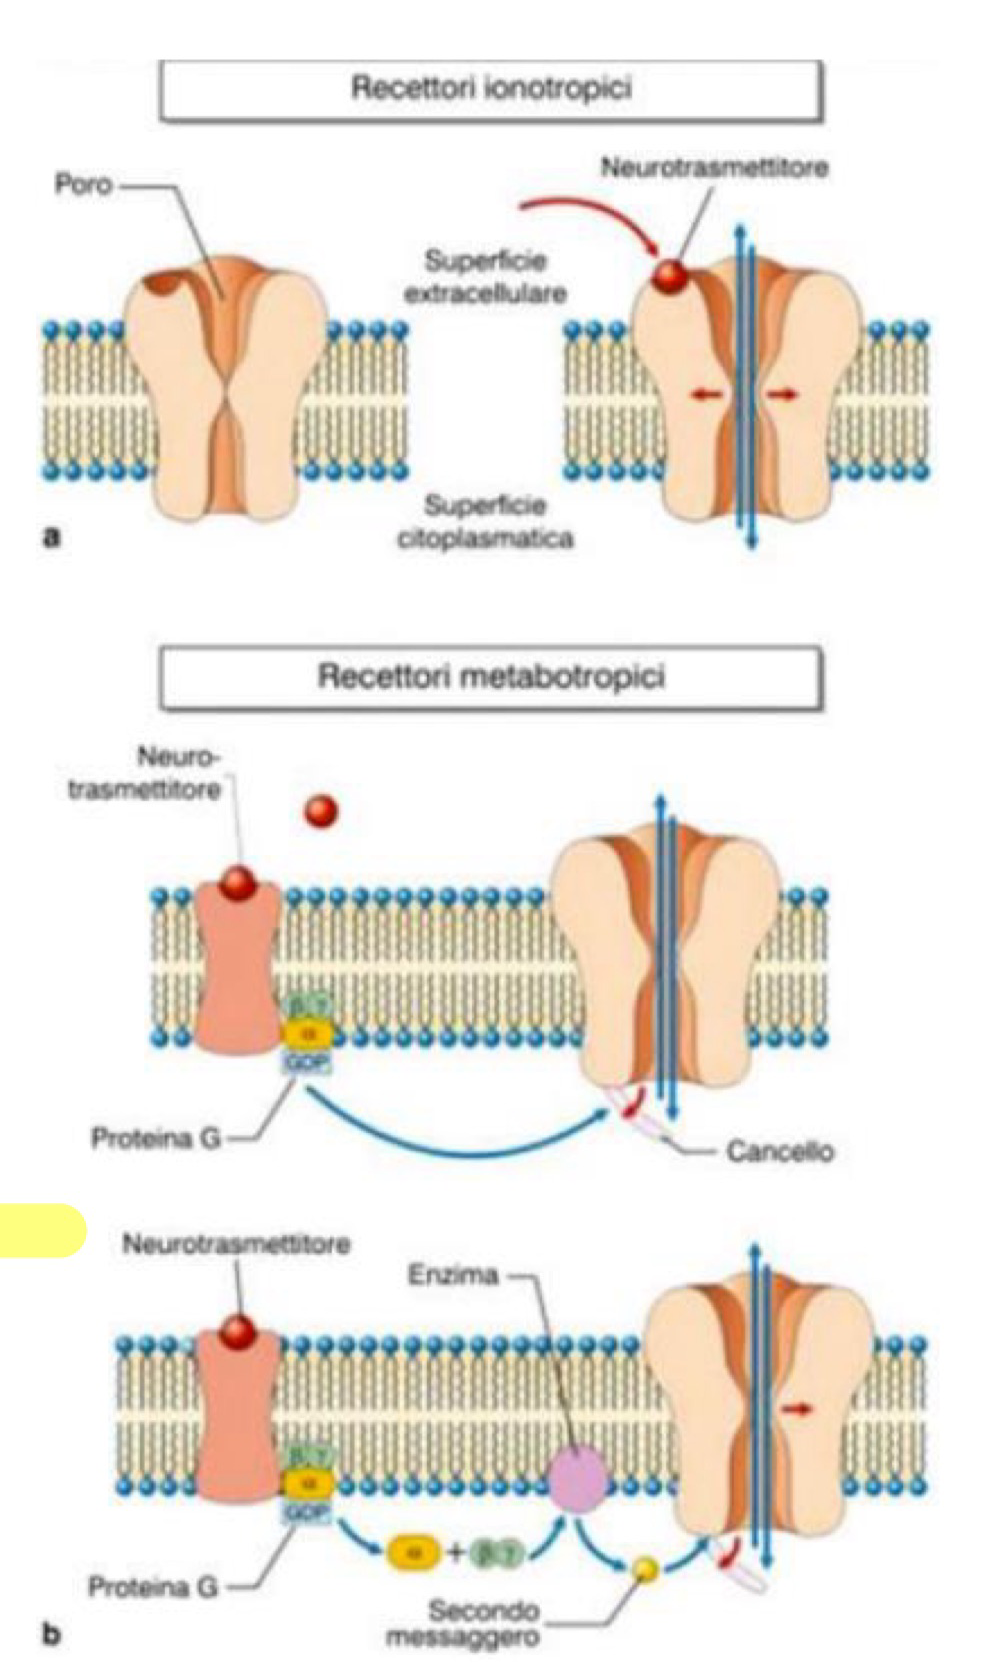
\includegraphics[width=0.80\textwidth]{images/image25.png}
\end{figure}

Come abbiamo detto, i meccanismi di apertura dei canali possono essere di due tipi: ionotropico e metabotropico.

Nel meccanismo \textbf{ionotropico }il canale ionico può essere immaginato come una serratura e il neurotrasmettitore come la chiave: appena arriva, il neurotrasmettitore interagisce direttamente con il canale e lo apre. In questo caso il recettore coincide con il canale stesso o si trova su di esso. Si tratta quindi di un meccanismo semplice e molto rapido (sia ad attivare che a riattivare il canale, per esempio il riflesso motorio).

Nel meccanismo \textbf{metabotropico}, invece, il processo è più complesso, perché c'è una mediazione tra il legame del neurotrasmettitore e l'apertura del canale. Possiamo immaginarlo come aprire una porta tramite un citofono: il neurotrasmettitore non si lega al canale ma a un recettore separato. Questo legame genera delle molecole dette secondi messaggeri, che si muovono all'interno della cellula e interagiscono con i canali a cancello, inducendone l'apertura. Questo meccanismo è più lento e complesso, ma consente un'ampia gamma di funzioni e comporta cambiamenti nel tempo (plasticità, esperienza, apprendimento e memoria).

\begin{figure}[htbp]
  \centering
  
\includegraphics[width=0.80\textwidth]{images/image26.png}
\end{figure}

\begin{figure}[htbp]
  \centering
  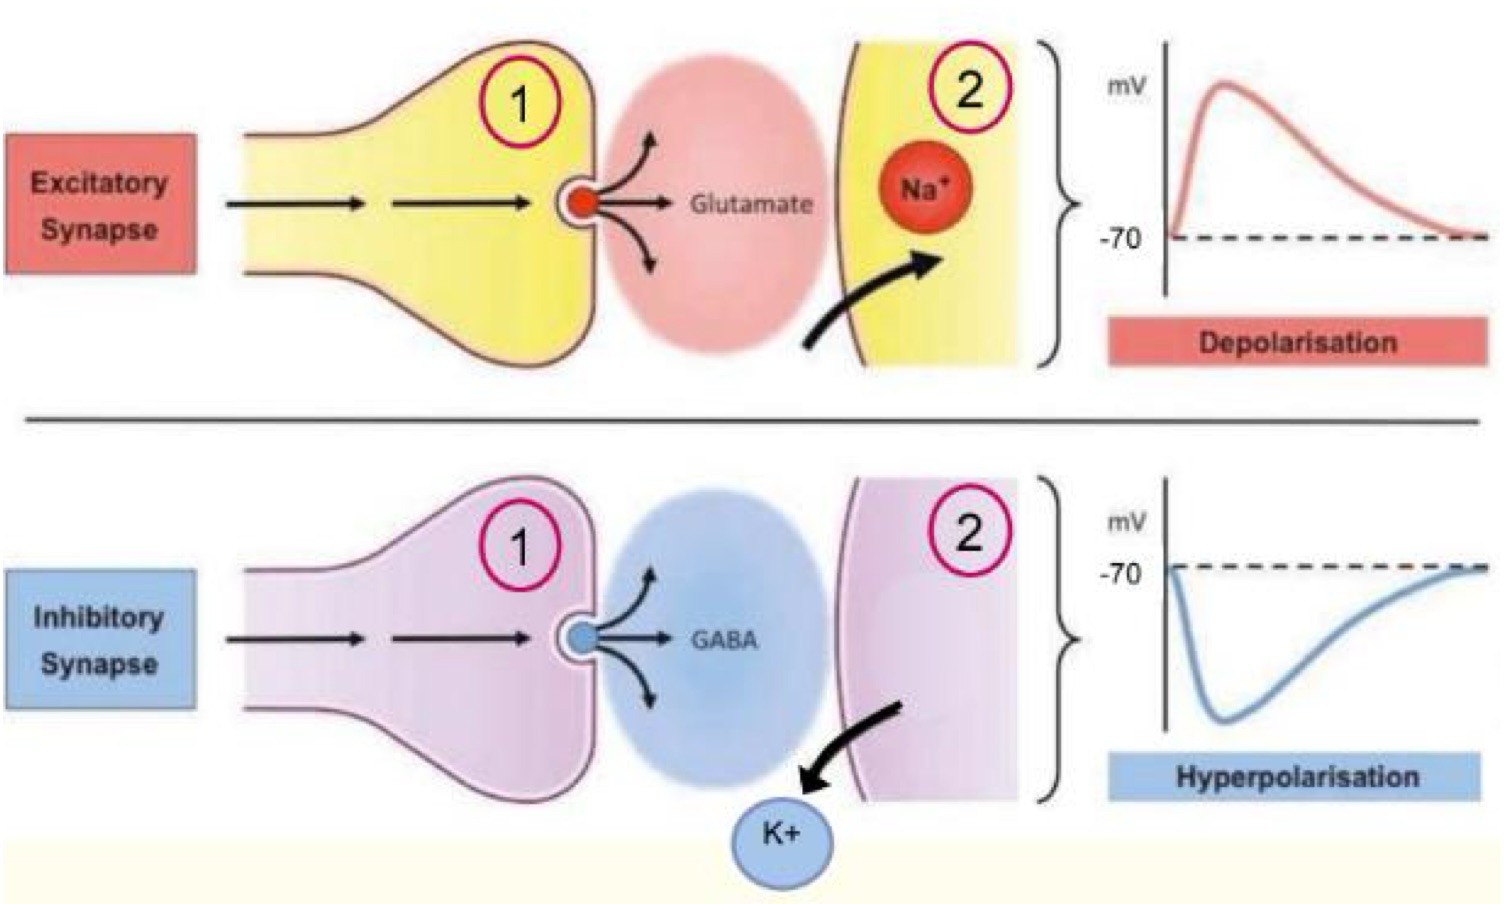
\includegraphics[width=0.80\textwidth]{images/image27.jpeg}
\end{figure}

Nelle sinapsi elettriche, poiché l'informazione è sempre una depolarizzazione (potenziale d'azione), l'unico effetto possibile sulla membrana post-sinaptica è una depolarizzazione: il segnale non può mai cambiare segno. Le sinapsi chimiche, invece, sono molto più flessibili e permettono una varietà di interazioni tra cellule. I vantaggi principali sono due: consentono variazioni del potenziale di membrana post-sinaptico sia in senso positivo sia in senso negativo, e permettono meccanismi di memoria.

Per quanto riguarda il primo vantaggio, consideriamo due casi. Nella prima situazione, quando un potenziale d'azione raggiunge il bottone sinaptico, viene rilasciato un neurotrasmettitore come il glutammato, che apre canali chimicamente controllati del sodio (sia ionotropici sia metabotropici). Questi canali sono passivi e permettono l'ingresso del sodio dall'esterno all'interno secondo gradiente elettrochimico, producendo una depolarizzazione della membrana post-sinaptica. Questa depolarizzazione è più lenta e meno ampia rispetto a un potenziale d'azione, e prende il nome di potenziale post-sinaptico eccitatorio (EPSP). È detto ``eccitatorio'' perché avvicina il potenziale di membrana alla soglia di apertura dei canali voltaggio-dipendenti del sodio, contribuendo così alla generazione di un potenziale d'azione, anche se da solo potrebbe non bastare.

Nel secondo caso, quando un potenziale d'azione raggiunge il bottone sinaptico, viene rilasciato un altro neurotrasmettitore, ad esempio il GABA, che apre i canali chimicamente controllati del potassio, esso tende a uscire dalla cellula post-sinaptica, producendo un'iperpolarizzazione della membrana. Il potenziale che ne deriva prende il nome di potenziale post-sinaptico inibitorio (IPSP), perché allontana il potenziale di membrana dalla soglia necessaria e quindi sfavorisce la generazione di un potenziale d'azione.

In sintesi, un potenziale post-sinaptico può essere eccitatorio o inibitorio a seconda dei canali che si aprono. Se si aprono i canali del sodio, si parla di sinapsi eccitatoria; se si aprono canali che hanno effetto iperpolarizzante, come quelli del potassio, si parla di sinapsi inibitoria. Anche il cloro partecipa in alcune sinapsi chimiche con canali chimicamente controllati: in genere ha effetto inibitorio, ma non in modo assoluto. Il potenziale di equilibrio del cloro è circa -65 mV, molto vicino al potenziale di membrana a riposo.

Infine, \textbf{cosa succede esattamente nella cellula post-sinaptica? }Quando il potenziale d'azione arriva al neurone pre-sinaptico, si ha una forte depolarizzazione della membrana che apre i canali del calcio. L'ingresso di calcio provoca il rilascio del neurotrasmettitore nella fessura sinaptica. Dall'altro lato, i recettori della cellula post-sinaptica riconoscono quella specifica molecola e, attraverso meccanismi ionotropici o metabotropici, inducono l'apertura dei canali ionici chimicamente controllati. Gli ioni, muovendosi secondo gradiente elettrochimico, determinano una variazione del potenziale: può essere depolarizzazione (se entra sodio) o iperpolarizzazione (se esce potassio).

L'iperpolarizzazione, cioè un contributo negativo, ha un ruolo importante. Infatti la cellula post-sinaptica non riceve un solo potenziale, ma moltissimi, e non da una sola sinapsi, ma da tante contemporaneamente. Anche considerando una sola sinapsi, il neurone non riceve un singolo impulso, ma una sequenza di potenziali d'azione a distanza variabile. L'informazione, quindi, risulta dalla somma e dall'integrazione di tanti segnali eccitatori e inibitori.

L'esistenza delle sinapsi inibitorie è fondamentale, perché interviene nella terza funzione della cellula, ovvero l'integrazione dell'informazione, che possiamo considerare come l'elaborazione dei segnali ricevuti. Integrare significa sommare: la cellula somma tutte le informazioni che riceve, e il risultato di questa somma costituisce una decisione. Questo processo avviene fisicamente grazie alla membrana cellulare, che ricopre l'albero dendritico e il soma fino al cono d'emergenza.

\begin{figure}[htbp]
  \centering
  
\includegraphics[width=0.80\textwidth]{images/image28.png}
\end{figure}

Per quanto riguarda la sommazione, si parte dai potenziali post-sinaptici, sia eccitatori sia inibitori. Per la cellula ricevente, l'informazione si manifesta come una variazione del potenziale di membrana in un punto specifico: in un punto si può avere una depolarizzazione di un certo valore, in un altro punto un'altra depolarizzazione, e così via.

\begin{figure}[htbp]
  \centering
  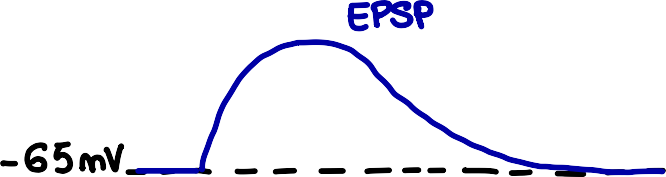
\includegraphics[width=0.80\textwidth]{images/image29.png}
\end{figure}

La sommazione avviene tramite due meccanismi: sommazione spaziale e sommazione temporale. Per comprendere il processo, consideriamo un caso teorico con una sola sinapsi e un solo potenziale d'azione. In un punto della membrana post-sinaptica arriva un potenziale d'azione e si verifica una sinapsi eccitatoria: il potenziale di membrana passa dal valore di riposo (-65 mV) a una variazione positiva di pochi millivolt. Questa ampiezza è troppo piccola per raggiungere la soglia necessaria all'apertura dei canali voltaggio-dipendenti (circa 1mV).

\begin{figure}[htbp]
  \centering
  
\includegraphics[width=0.80\textwidth]{images/image31.png}
\end{figure}

Dopo un breve intervallo, in assenza di altre perturbazioni, la membrana ritorna all'equilibrio grazie alle pompe sodio-potassio. In pratica, i canali si chiudono, il potenziale d'azione fa entrare ioni sodio, i canali poi si richiudono, e la pompa sodio-potassio ripristina l'equilibrio spostando dentro ioni potassio e fuori ioni sodio. L'intero processo richiede circa 10--15 millisecondi.

Nella realtà, però, si hanno tante sinapsi. Valutiamo quindi i meccanismi che avvengono:

\begin{figure}[htbp]
  \centering
  
\includegraphics[width=0.80\textwidth]{images/image33.png}
\end{figure}

La sommazione spaziale si verifica quando più sinapsi eccitatorie, poste in punti vicini nello spazio, producono perturbazioni che si propagano nelle regioni circostanti e finiscono per agire insieme. In

\begin{figure}[htbp]
  \centering
  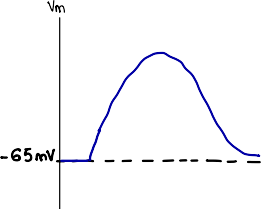
\includegraphics[width=0.80\textwidth]{images/image34.png}
\end{figure}

questo caso gli ioni positivi entrano attraverso ciascuna sinapsi e la quantità totale di cariche positive all'interno della membrana risulta moltiplicata rispetto a quella prodotta da una sola sinapsi. Di conseguenza, l'ampiezza della curva che descrive il fenomeno è maggiore, e cresce ulteriormente se le sinapsi coinvolte sono numerose, ad esempio un centinaio. Questo avviene perché i potenziali post-sinaptici hanno una durata molto più lunga rispetto a quella del potenziale d'azione: prima che tornino all'equilibrio, c'è tempo per l'arrivo di numerosi potenziali d'azione. Si parla dunque di meccanismo spaziale, nel quale la cellula somma in modo passivo gli effetti generati da più sinapsi vicine.

Se però tra queste sinapsi ve ne sono anche di tipo inibitorio, l'effetto cambia. Nel caso di due sinapsi eccitatorie e una inibitoria, le cariche negative introdotte da quest'ultima si sommano a

\begin{figure}[htbp]
  \centering
  
\includegraphics[width=0.80\textwidth]{images/image35.png}
\end{figure}

quelle positive delle prime, con un risultato finale meno marcato rispetto alla sommazione di tre eccitatorie. Se invece sono presenti due sinapsi inibitorie e una eccitatoria, il risultato è un'iperpolarizzazione. Infine, la distanza della sinapsi dal cono d'emergenza dell'assone è un fattore importante. Una sinapsi lontana produce un effetto molto più debole rispetto a una vicina, perché durante il trasporto e la sommazione l'informazione può attenuarsi o perdersi. Diventano quindi fondamentali la geometria e l'estensione fisica della cellula nel determinare l'efficacia della sommazione spaziale.

\begin{figure}[htbp]
  \centering
  
\includegraphics[width=0.80\textwidth]{images/image36.png}
\end{figure}

La sommazione temporale dipende dal fatto che i potenziali d'azione arrivano sulla stessa sinapsi in sequenza, più o meno ravvicinati nel tempo. Supponiamo di avere una sinapsi eccitatoria su cui arrivano tre potenziali d'azione molto vicini tra loro. Se ne arrivasse solo uno, si osserverebbe un singolo andamento del potenziale post-sinaptico, ma quando sono più di uno, il secondo potenziale arriva mentre il primo è ancora in corso, quindi la membrana non è tornata al riposo. In questo modo il secondo potenziale si somma al primo, causando un ulteriore aumento della depolarizzazione, in un meccanismo graduato. Lo stesso avviene con il terzo potenziale: ciascuno arriva su una membrana già parzialmente polarizzata, amplificando l'effetto complessivo. Alla chiusura dei canali ionici, infine, la membrana torna all'equilibrio. Se la sinapsi fosse inibitoria, il grafico sarebbe lo

\begin{figure}[htbp]
  \centering
  
\includegraphics[width=0.80\textwidth]{images/image39.png}
\end{figure}

stesso ma invertito, mostrando iperpolarizzazione anziché depolarizzazione. Se invece i potenziali d'azione arrivano distanziati nel tempo, la sommazione non si verifica perché ciascun potenziale ha il

tempo di riportare la membrana al riposo prima dell'arrivo del successivo.

\begin{figure}[htbp]
  \centering
  
\includegraphics[width=0.80\textwidth]{images/image40.png}
\end{figure}

Si consideri una cellula post-sinaptica con due sinapsi: quella in alto, eccitatoria, e quella in basso, inibitoria. Immaginiamo di misurare i potenziali di membrana con tre elettrodi posti lungo lo stesso asse temporale: uno in alto sulla cellula pre-sinaptica della sinapsi eccitatoria, uno nel mezzo sulla cellula che fa la sinapsi inibitoria e uno in basso sulla cellula ricevente. In questo esempio, sulla cellula eccitatoria arrivano quattro potenziali d'azione e uno solo sulla sinapsi inibitoria. All'inizio arriva un potenziale eccitatorio isolato, che non si somma con altri e porta la membrana a tornare rapidamente all'equilibrio. Successivamente, due potenziali d'azione ravvicinati sulla sinapsi eccitatoria si sommano temporalmente, aumentando il potenziale post-sinaptico fino a raggiungere la soglia dei canali del sodio voltaggio-dipendenti e generando un potenziale d'azione. Quando arriva simultaneamente un potenziale eccitatorio e uno inibitorio, i due effetti si bilanciano tra loro, annullandosi quasi completamente. In questo modo, i meccanismi di sommazione temporale e spaziale agiscono insieme: l'effetto della sommazione temporale si somma spazialmente con quello di altre sinapsi. Moltiplicando questo fenomeno per migliaia di sinapsi e per un numero elevatissimo di potenziali d'azione nel tempo, si ottiene una variazione del potenziale post-membrana che può assumere forme molto diverse, senza un andamento tipico.

L'output binario della cellula è costituito dalla sequenza dei potenziali d'azione. Nell'esempio considerato, si osservano quattro sinapsi e quattro treni di potenziali diversi. L'informazione passa dalla cellula pre-sinaptica a quella post-sinaptica tramite una sinapsi chimica. Sulla membrana post-sinaptica si osserva quindi l'effetto della sommazione temporale o spaziale, il cui risultato è rappresentato nel grafico.

L'intervallo temporale considerato è di circa 10 millisecondi.

\begin{figure}[htbp]
  \centering
  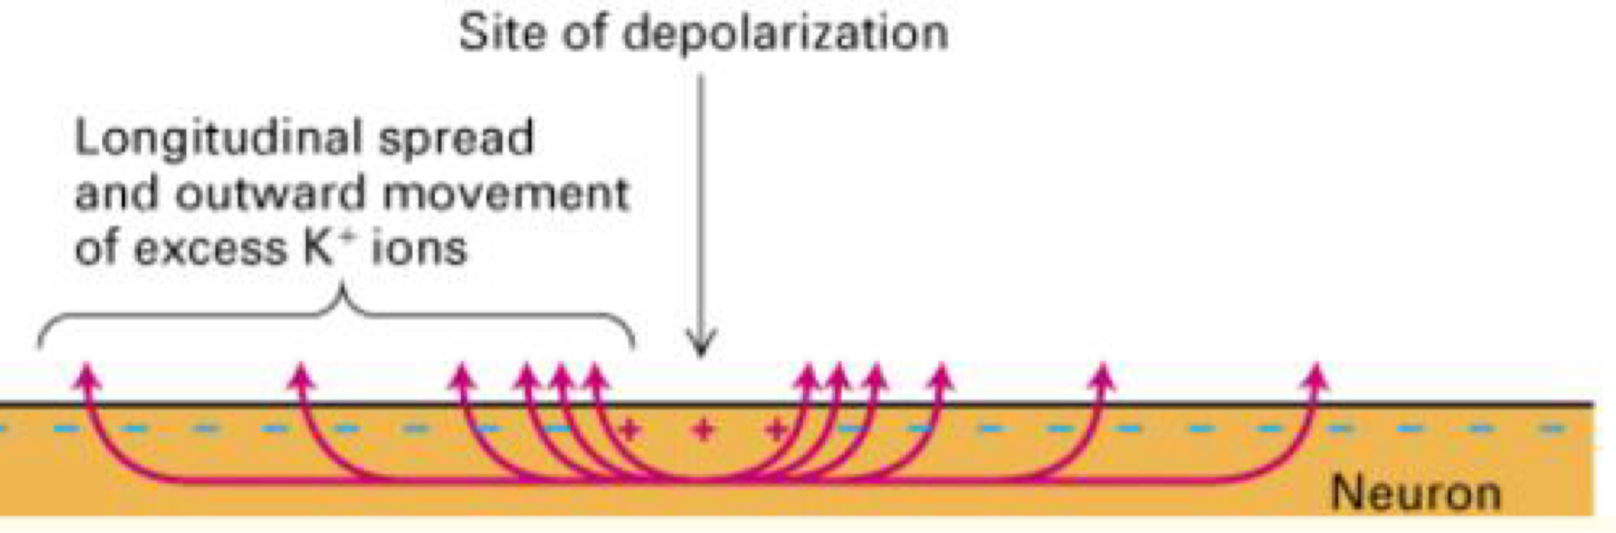
\includegraphics[width=0.80\textwidth]{images/image43.png}
\end{figure}

Le perturbazioni di cui si è parlato in precedenza corrispondono ai potenziali post-sinaptici sommati tra loro, che producono una variazione del potenziale di membrana. Localmente si osserva una depolarizzazione: la membrana in quella zona diventa meno negativa rispetto alle altre regioni, ma questo non significa che diventi positiva, semplicemente che la negatività è ridotta. Le cariche concentrate, essendo libere di muoversi nel liquido intracellulare, generano correnti intracellulari che propagano la perturbazione ai siti vicini. Questa propagazione è passiva, non direzionata e dipende dalla distanza dal punto di origine del potenziale. Grazie a questo meccanismo, la sommazione spaziale può avvenire anche quando le sinapsi non sono direttamente adiacenti tra loro, e permette al risultato finale di raggiungere il cono d'emergenza dell'assone.

I potenziali post sinaptici sommati tra loro prendono il nome di potenziali graduati. I potenziali d'azione hanno sempre lo stesso segno positivo e risultano quindi sempre depolarizzanti, a differenza dei potenziali graduati, che possono essere sia depolarizzanti che iperpolarizzanti. Per farsi che si generi un potenziale d'azione è necessario raggiungere un valore soglia, mentre nei potenziali graduati questo non è richiesto. I potenziali d'azione eseguono il principio del tutto o nulla, mentre negli altri l'intensità dello stimolo influisce sull'ampiezza del segnale. Per quanto riguarda la propagazione, i potenziali d'azione si diffondono in maniera continua o saltatoria, i graduati invece si propagano solo passivamente e non si rigenerano mai, percorrendo distanze minori. Inoltre i potenziali d'azione presentano un periodo refrattario assoluto e un periodo refrattario relativo, assenti in quelli graduati. I potenziali d'azione caratterizzano in modo specifico le cellule eccitabili, come quelle nervose, muscolari e cardiache, mentre i graduati possono essere presenti in tutte le cellule.

\begin{figure}[htbp]
  \centering
  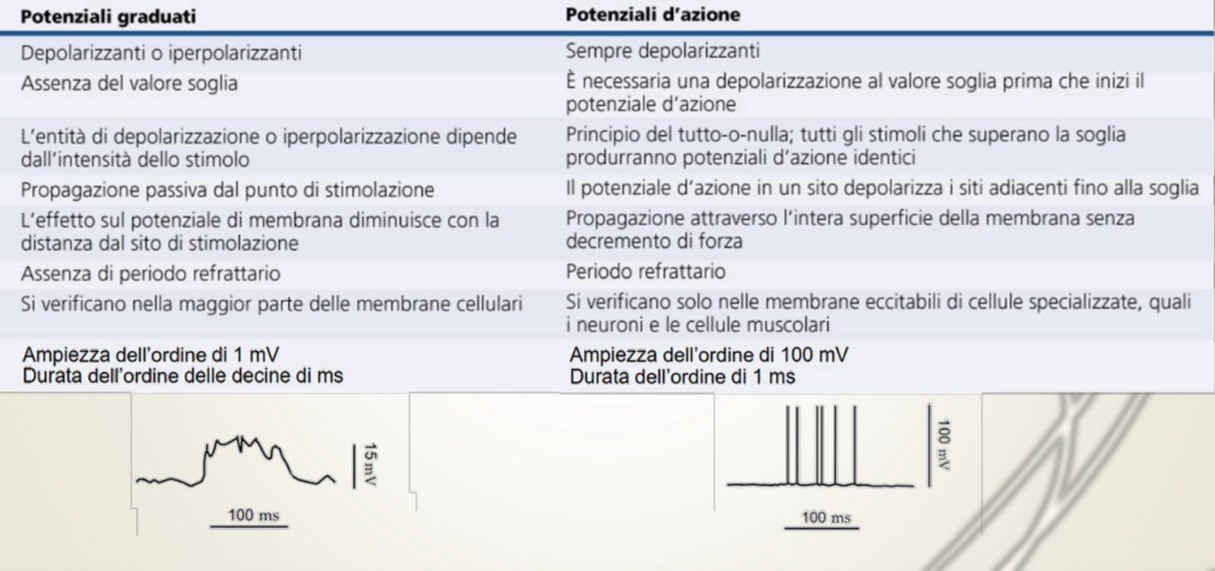
\includegraphics[width=0.80\textwidth]{images/image44.jpeg}
\end{figure}

L'integrazione dell'informazione nella membrana avviene tramite la sommazione degli EPSP e degli IPSP, sia spaziale che temporale. Questo determina la depolarizzazione o l'iperpolarizzazione della membrana: se la depolarizzazione non raggiunge la soglia o se prevale l'iperpolarizzazione, il potenziale d'azione non si genera. Il segnale risultante si propaga passivamente fino al cono d'emergenza dell'assone, dove può nascere il potenziale d'azione. La possibilità di raggiungere la soglia dipende dall'intensità della perturbazione e dalla geometria dei dendriti, in particolare dalla loro distanza e posizione rispetto al cono d'emergenza, poiché l'effetto si attenua con la distanza.

\begin{figure}[htbp]
  \centering
  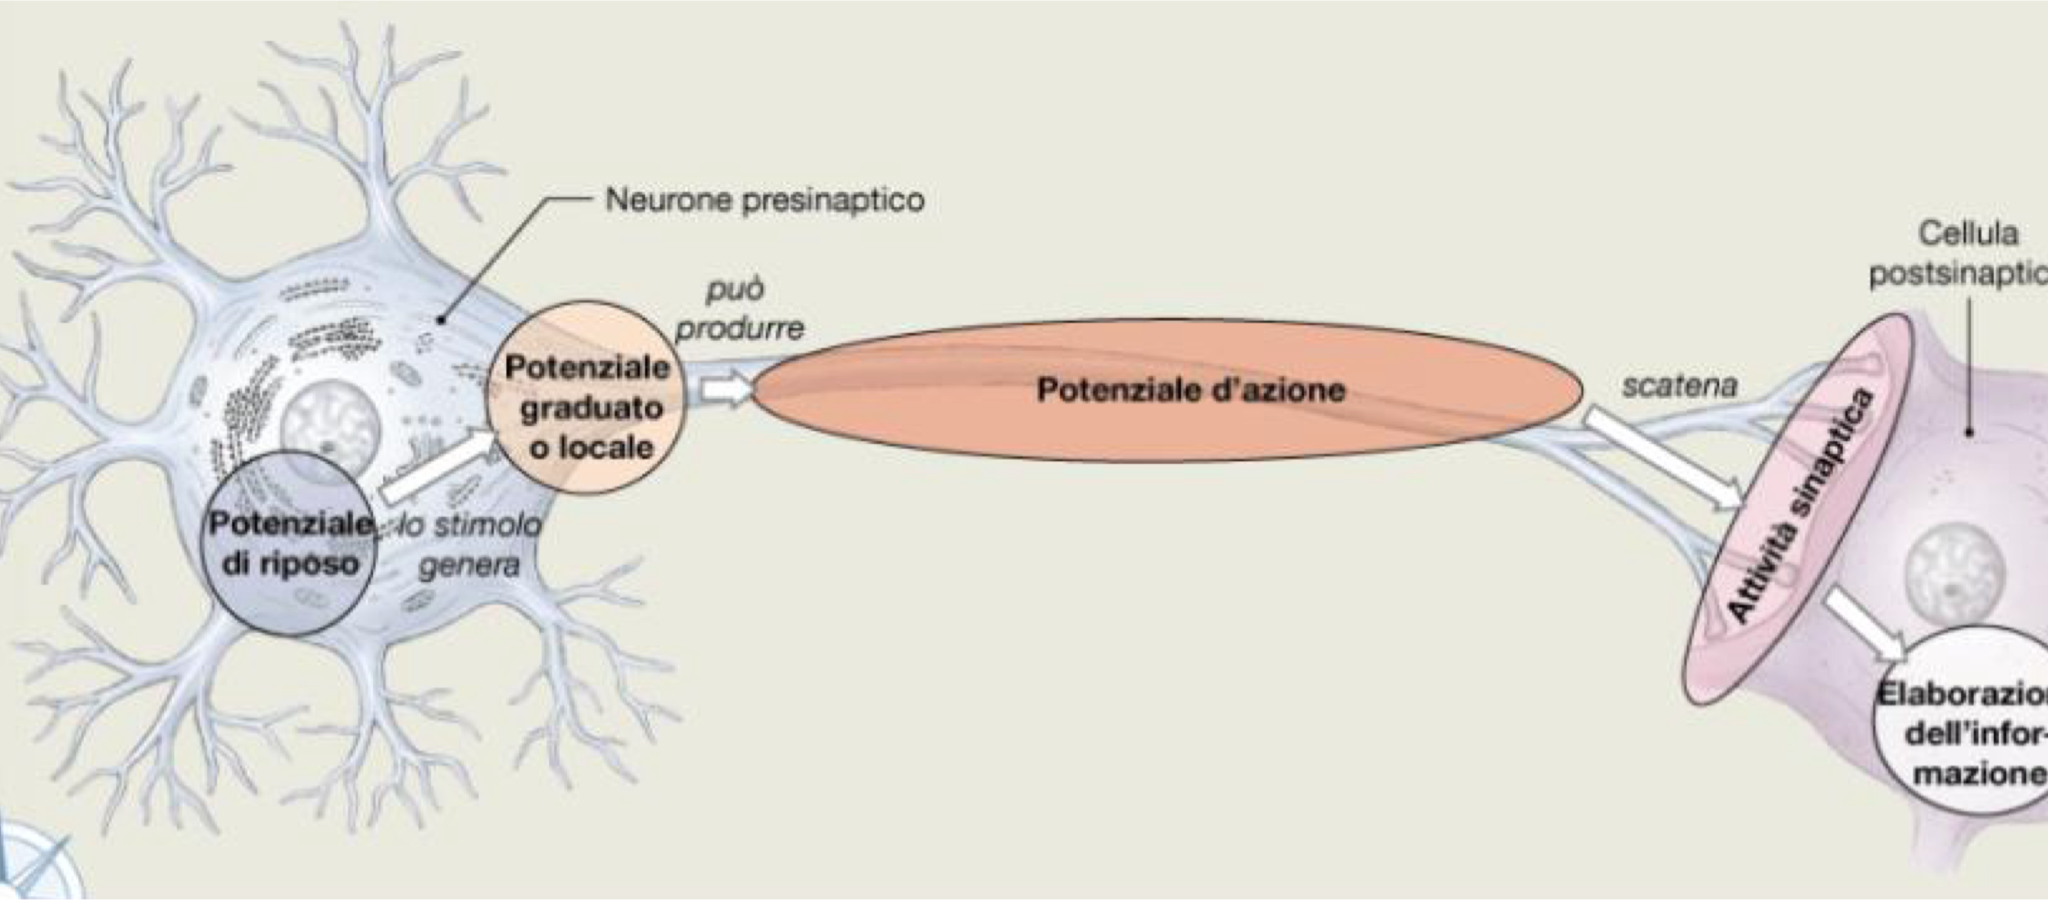
\includegraphics[width=0.80\textwidth]{images/image49.png}
\end{figure}

All'interno della cellula, che possiede un potenziale di riposo, gli stimoli ricevuti dai dendriti con segno positivo o negativo producono, tramite sommazione spaziale o temporale, un potenziale graduato o locale. Se questo potenziale supera la soglia, viene generato un potenziale d'azione, che si propaga lungo l'assone in maniera continua o saltatoria fino alla sua estremità. La cellula comunica con altre tramite sinapsi, di solito chimiche, che possono essere eccitatorie o inibitorie: in base al neurotrasmettitore rilasciato, si genera un potenziale d'azione eccitatorio o inibitorio nella cellula successiva.

\textbf{CAP1. REGISTRAZIONE DELLA RISPOSTA NEURALECAP1. REGISTRAZIONE DELLA RISPOSTA NEURALE}

\textbf{1d. Registrazioni intra ed extra cellulari}

Le registrazioni intracellulari permettono di misurare direttamente il potenziale attraverso la membrana cellulare. Per farlo si utilizza un elettrodo di riferimento, posizionato all'esterno, e un elettrodo perforante, che deve acquisire il potenziale dall'interno della cellula. Questo può avvenire in due modi: perforando fisicamente la membrana con l'elettrodo e attraversandola, oppure utilizzando un elettrodo che si fonde con la membrana entrando in contatto elettrico con la cellula. L'elettrodo perforante è solitamente una micropipetta di vetro riempita di soluzione salina concentrata, al cui interno vengono inseriti fili metallici collegati a un oscilloscopio. Quest'ultimo permette di visualizzare l'ampiezza del potenziale di membrana in Volt. Lo stesso avviene per l'elettrodo extracellulare: la differenza tra interno ed esterno della cellula rappresenta infatti il potenziale di membrana. Rispetto a un elettrodo patch, quello perforante è più complesso da utilizzare e presenta un rischio maggiore di danneggiare la membrana. Questo perché attraversarla senza comprometterla è un'operazione molto delicata: è più semplice in alcune zone della cellula, come nel soma o in certe parti dell'albero dendritico, e molto più difficile negli assoni o nelle ramificazioni sottili. A questa difficoltà si aggiunge il problema delle registrazioni in vivo, dove occorre raggiungere i neuroni nel cervello senza danneggiare il tessuto circostante. Le registrazioni intracellulari possono quindi essere effettuate in vivo, cioè direttamente nel cervello, oppure in vitro, estraendo i neuroni e studiandoli in laboratorio. In quest'ultimo caso, poiché i neuroni non si trovano più nel loro ambiente naturale, è necessario stimolarli artificialmente con iniezioni di corrente che simulano l'effetto delle sinapsi, così da osservare le loro risposte. Questo rappresenta un compromesso utile quando le registrazioni in vivo non sono possibili.

Il grande vantaggio delle registrazioni intracellulari è che consentono di misurare in modo diretto e preciso l'attività neuronale, cioè l'andamento nel tempo del potenziale di membrana. Dal punto di vista della qualità del segnale non esistono tecniche equiparabili: l'unico modo per avere una misura diretta dell'attività neuronale è proprio questo tipo di registrazione.

Le registrazioni extracellulari evitano l'aspetto più complesso delle registrazioni intracellulari, cioè l'attraversamento della membrana. Questo è possibile perché, quando nella cellula avvengono delle perturbazioni e si generano correnti intracellulari, all'esterno si creano correnti simmetriche ma di segno opposto. In questo modo, ponendo un elettrodo al di fuori della cellula e confrontandolo con un altro punto di riferimento, è possibile rilevare una differenza che indica che qualcosa sta accadendo, anche se in maniera meno chiara rispetto a quanto si osserva all'interno.

Il grande vantaggio di questa tecnica è che non si deve attraversare la membrana, evitando così il rischio di danneggiare la cellula. Non ci si scontra quindi con il problema delle porzioni sottili e fragili della membrana, e si può registrare vicino a

strutture come assoni o dendriti. Anche in vivo l'operazione risulta più semplice. Lo svantaggio, invece, riguarda la qualità del segnale: con questa tecnica non si misura direttamente il potenziale di membrana, ma solo variazioni importanti di

esso. Più grande è la variazione, più è probabile che venga rilevata anche con un elettrodo esterno. Questo significa che non si misura l'attività neuronale in senso stretto, ma si riescono a rilevare solo i fenomeni più intensi, cioè i potenziali d'azione, e non quelli graduati. Infatti, le variazioni dei potenziali graduati sono spesso così piccole da confondersi con il rumore, mentre quelle dei potenziali d'azione sono sempre evidenti e certe. Questa tecnica viene quindi utilizzata esclusivamente per rilevare l'avvenuto potenziale d'azione e per sapere in quale istante esso si verifica. Non si misura la sua ampiezza, ma non è un problema, perché il potenziale d'azione ha sempre la stessa grandezza. L'informazione non è contenuta nell'ampiezza o nell'andamento, ma nella frequenza con cui i potenziali d'azione appaiono. Ad esempio, se in un secondo si hanno cinque potenziali d'azione, nel caso in cui siano ravvicinati tra loro, a distanza di 3 millisecondi, si ha una sommazione temporale che produce un effetto maggiore sul neurone ricevente. Se invece sono distanziati, l'effetto risulta più blando.

In sintesi, quando si vuole studiare l'attività dei potenziali d'azione ci sono due possibilità: se si vogliono indagare i meccanismi di generazione del potenziale, occorre misurarne l'andamento nel tempo, e quindi non si possono usare le registrazioni extracellulari, ma servono quelle intracellulari, come nel classico esperimento sull'assone gigante. Se invece non si è interessati all'ampiezza o all'andamento, ma solo a verificare se una cellula in un certo momento stia producendo o meno un potenziale d'azione, allora la registrazione extracellulare è sufficiente. Questo non vale per i potenziali graduati, perché troppo piccoli per essere rilevati con questa tecnica.

\begin{figure}[htbp]
  \centering
  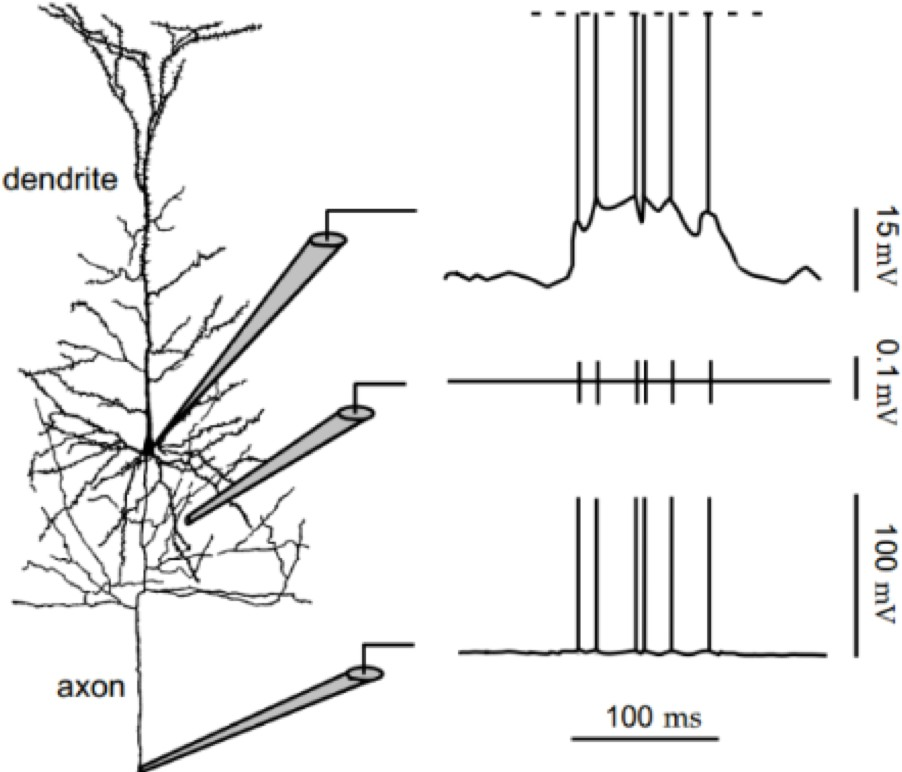
\includegraphics[width=0.80\textwidth]{images/image50.jpeg}
\end{figure}

In figura è rappresentato un neurone piramidale, così chiamato perché il soma ha una forma piramidale. Sono state effettuate tre registrazioni simultanee sullo stesso neurone, confrontando i risultati.

La prima registrazione è intracellulare e viene fatta sul soma, vicino al cono di emergenza dell'assone. In questo punto è possibile misurare sia i potenziali d'azione sia i potenziali graduati, perché l'elettrodo entra direttamente in contatto con l'interno della cellula. Nel grafico, i potenziali d'azione appaiono tagliati a causa della scala utilizzata. La seconda registrazione è extracellulare. Qui l'elettrodo viene posto vicino all'assone e permette di rilevare con precisione gli istanti in cui si verificano i potenziali d'azione, ma non di misurarne l'ampiezza reale. Inoltre, i potenziali graduati non vengono registrati, perché l'elettrodo non è abbastanza sensibile. In questo caso, nel grafico l'ampiezza rilevata è di circa 0,1 mV, molto più piccola di quella reale.

La terza registrazione è intracellulare, ma fatta direttamente sull'assone. In questo modo si entra a contatto con l'ambiente cellulare e si rilevano i potenziali d'azione, ma non i potenziali graduati. Confrontando i tre grafici, si osserva che le ampiezze registrate sono molto diverse tra loro: nella registrazione extracellulare, l'ampiezza appare molto ridotta rispetto al valore reale, quindi non si può dire di aver misurato effettivamente il potenziale. Inoltre, nell'assone non compaiono i potenziali graduati. Ciò che rimane uguale in tutte e tre le registrazioni è l'istante in cui i potenziali d'azione si verificano. Quando si devono effettuare delle registrazioni, la prima domanda da porsi è a cosa serva la misura. Se si vuole vedere se la cellula risponde a stimoli interni attraverso i potenziali graduati, la registrazione extracellulare deve essere esclusa. Se invece interessa solo verificare la presenza dei potenziali d'azione, allora la registrazione extracellulare può essere sufficiente. Un'altra considerazione riguarda il contesto: una registrazione in vivo è molto più difficile da realizzare rispetto a una in vitro. In conclusione, la scelta tra registrazione intracellulare o extracellulare dipende dalla localizzazione, dal tipo di segnale che si vuole acquisire e dalla possibilità o meno di stimolare il neurone. Per esempio, se si vuole osservare la risposta di una cellula a un certo stimolo e descrivere il trend dei potenziali che produce, si userà una registrazione extracellulare. Se invece si vogliono studiare i meccanismi di generazione del potenziale d'azione, sarà necessario ricorrere a una registrazione intracellulare in vitro.

\begin{figure}[htbp]
  \centering
  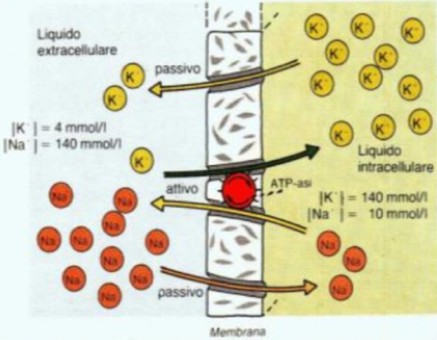
\includegraphics[width=0.80\textwidth]{images/image51.jpeg}
\end{figure}

\chapter{Modelli elettrici della membrana neuronale}

\section{2a. Introduzione ai modelli elettrici di membrana}

\textbf{2a. INTRODUZIONE AI MODELLI ELETTRICI DI MEMBRANA2a. INTRODUZIONE AI MODELLI ELETTRICI DI MEMBRANA}

Le caratteristiche fisiche della membrana cellulare possono essere tradotte in proprietà

elettriche, utilizzando dei \textbf{circuiti elettrici come rappresentazione astratta di fenomeni }che, nella realtà, hanno natura fisica. Questo tipo di modello risulta uno strumento adeguato a rappresentare la membrana di cellule eccitabili in quanto, quest'ultima, svolge le proprie funzioni tramite la \textbf{variazione di grandezze elettriche }(come il potenziale di membrana o la corrente di membrana).

Le correnti ioniche che attraversano la membrana possono essere attivate da:

\begin{itemize}
  \item \textbf{Canali di membrana}: non selettivi, selettivi o controllati (a cancello). Possono essere \textit{canali variabili }in base a specifici stimoli o \textit{canali sempre aperti}, che permettono il passaggio di ioni secondo gradiente elettrochimico (trasporto passivo);
  \item \textbf{Pompe ioniche}: dove, invece, gli ioni vengono spostati contro gradiente di concentrazione, utilizzando energia (trasporto attivo).
\end{itemize}
\textbf{LIVELLO DI ASTRAZIONE}

L'obiettivo principale è quello di \textbf{passare dalla struttura reale del neurone }(in figura 1) \textbf{ad un modello di esso }(in figura 4), che ovviamente non dovrà essere fedele al progetto fisico. Questo perché bisogna utilizzare uno schema utile ai nostri scopi, fornendo le informazioni corrette.


\subsection{Neurone biologico completo}

Viene rappresentato un neurone realistico, con tutti i suoi tratti fisiologici principali (soma, albero dendritico, assone e terminali assonici). Non è utile in questo caso perché è una struttura troppo complessa per poter essere modellata direttamente;


\subsection{Semplificazione a compartimenti}

Schematizzazione del neurone con \textbf{segmenti rettilinei }connessi tra loro, come rappresentazione delle ramificazioni dendritiche. Abbiamo poi le sinapsi ancora visibili, rappresentate da \textbf{triangolini }ed infine il colle dell'assone, rappresentato da un \textbf{cerchio};


\subsection{Modello semplificato a pochi rami}

Le precedenti ramificazioni dendritiche sono adesso rappresentate da \textbf{pochi rami principali }più grandi. Le sinapsi sono ancora visibili in quanto è necessario che l'informazione si propaghi;


\subsection{Modello a punto singolo (one-compartment model)}

Si arriva ad una situazione di estrema semplificazione, dove il cono di emergenza dell'assone è rappresentato da una \textbf{sfera }e le sinapsi si trovano tutte vicine tra loro \textbf{come se si fondessero in un unico punto}. Questo modello è detto ``\textbf{\textit{a}}\textbf{\textit{ }}\textbf{\textit{punto}}'' o ``\textbf{\textit{integratore}}'': non si considera più la distribuzione spaziale ma solo l'attività globale e tutte le sinapsi contribuiscono alla stessa variabile di membrana.

\subsubsection{Modello a singolo compartimento}

Il modello a singolo compartimento non è così tanto lontano dalla realtà, infatti, ricorda molto le \textit{registrazioni intracellulari}, dove il potenziale viene misurato solo in un punto del neurone, assumendo che esso rappresenti bene l'intero compartimento cellulare.

Si andranno a \textbf{trascurare le variazioni del potenziale di membrana nello spazio}, poiché sono state eliminate con la modellizzazione fatta in precedenza. A questo punto, quindi, è possibile descrivere le grandezze elettriche con un \textbf{unico valore rispetto alla dimensione spaziale}: un unico valore per il potenziale di membrana (costante nello spazio) e uno per le correnti di membrana.

Gli elementi circuitali equivalenti che verranno utilizzati nel modello sono:

\begin{itemize}
  \item Resistenza $\rightarrow$ canali ionici;
  \item Condensatore $\rightarrow$ capacità della membrana di accumulare cariche.
\end{itemize}
\textbf{OSS: }per svincolarsi dalle dimensioni della membrana ogni grandezza elettrica sarà per ora riferita all'unità di spazio.

\subsubsection{Proprieta' capacitive della membrana}

La membrana è costituita da un \textbf{doppio strato fosfolipidico }che separa due ambienti con distribuzione di cariche differenti: \textbf{cariche negative }disposte all'interno della membrana e \textbf{cariche positive }all'esterno.

Il comportamento elettrico del doppio strato fosfolipidico può essere modellizzato con un \textbf{condensatore}, infatti, si osservano due superfici separate da una \textit{distanza d }(spessore del doppio strato fosfolipidico) su cui supponiamo essere distribuite le cariche dell'ambiente intra ed extra-cellulare.

Per svincolarsi dalla dimensione spaziale, nel circuito è conveniente, anziché calcolare la capacità del condensatore, dividere quest'ultima per la superficie della membrana (A): si ottiene così la \textbf{capacità specifica di membrana}.

\[
C_m = c_m \cdot A \qquad \text{(capacità totale, nF)}
\]
\[
c_m = \frac{C_m}{A} \qquad \text{(capacità specifica, nF/mm}^2\text{)}
\]

\textbf{EQUAZIONE DI BASE DELLA MEMBRANA}

A questo punto è possibile scrivere l'equazione di base del circuito partendo dal condensatore. La corrente capacitiva è:
\[
I_{cap} = C_m \frac{dV}{dt}
\]
dove $V$ è la differenza di potenziale di membrana (costante nello spazio ma variabile nel tempo).

\subsubsection{Proprietà resistive della membrana}

Il comportamento elettrico della membrana dipende principalmente dall'attività dei canali ionici e delle pompe ioniche. Un canale che permette il passaggio di ioni si modella con una \textbf{resistenza/conduttanza}.

Se molti canali sono aperti la resistenza è bassa; se sono chiusi la resistenza è praticamente infinita.

\textbf{OSS:} farmaci/tossine che bloccano i canali aumentano la resistenza di membrana, ostacolando la trasmissione nervosa.

\begin{itemize}
  \item \textbf{Conduttanza di membrana} $G_m = g_m \cdot A$ (S)
  \item \textbf{Conduttanza specifica} $g_m$ (S/mm$^2$)
  \item \textbf{Resistenza di membrana} $R_m = 1/G_m$ ($\Omega$)
  \item \textbf{Resistenza specifica} $r_m = 1/g_m$ ($\Omega\cdot$mm$^2$)
\end{itemize}

\textbf{EQUAZIONE DI NERNST -- richiamo}

Per ciascuna famiglia ionica si confronta il potenziale di equilibrio $E_j$ con il potenziale di membrana $V$ per capire la spinta che agisce sugli ioni: se $E_j$ è più negativo di $V$ si avrà un effetto \textit{iperpolarizzante}; se $E_j$ è meno negativo di $V$ l'effetto sarà \textit{depolarizzante}.

Inoltre, il potenziale di Nernst indica verso quale valore tende a spostarsi il potenziale di membrana a causa di quello ione.

\begin{figure}[htbp]
  \centering
  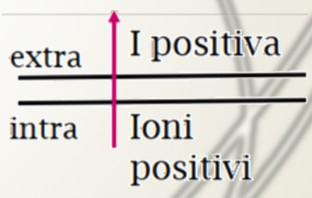
\includegraphics[width=0.80\textwidth]{images/image56.jpeg}
\end{figure}

\begin{itemize}
  \item $V < E_j$: correnti positive entrano $\rightarrow$ depolarizzazione;
  \item $V > E_j$: correnti positive escono $\rightarrow$ iperpolarizzazione/ripolarizzazione;
  \item Sinapsi eccitatorie: $V_m < E_j$ (depolarizzanti);
  \item Sinapsi inibitorie: $V_m > E_j$ (iperpolarizzanti).
\end{itemize}

\subsubsection{Corrente di membrana}

La \textbf{corrente di membrana} $i_m$ è il movimento netto di ioni attraverso la membrana (per unità di superficie). Convenzionalmente:
\begin{itemize}
  \item positiva $\rightarrow$ ioni positivi escono dalla cellula;
  \item negativa $\rightarrow$ ioni positivi entrano nella cellula.
\end{itemize}
Per gli ioni negativi la direzione è opposta.

La corrente ionica di una specifica famiglia $j$ si scrive:
\[
i_j = g_j\,(V - E_j)
\]
dove $g_j$ è la conduttanza specifica del canale per lo ione $j$, $E_j$ il suo potenziale di equilibrio.

\textbf{OSS: } tutte le correnti sono per unità di superficie.

\subsubsection{Conduttanze di membrana}

Le conduttanze di membrana possono essere suddivise in:

\begin{itemize}
  \item \textbf{Conduttanze costanti nel tempo}: dovute alle \textbf{pompe ioniche} o ai \textbf{canali ionici} \textit{sempre aperti} (rappresentati da un resistore in serie ad un generatore). Le pompe spostano ioni contro gradiente, quindi non vale l'equazione di Nernst; possono comunque essere rappresentate con rami resistivi senza generatore.
  \item \textbf{Conduttanze variabili nel tempo}: canali voltaggio-dipendenti o chimico-dipendenti. Sono funzioni del potenziale di membrana $V$ e del tempo.
\end{itemize}

\begin{figure}[htbp]
  \centering
  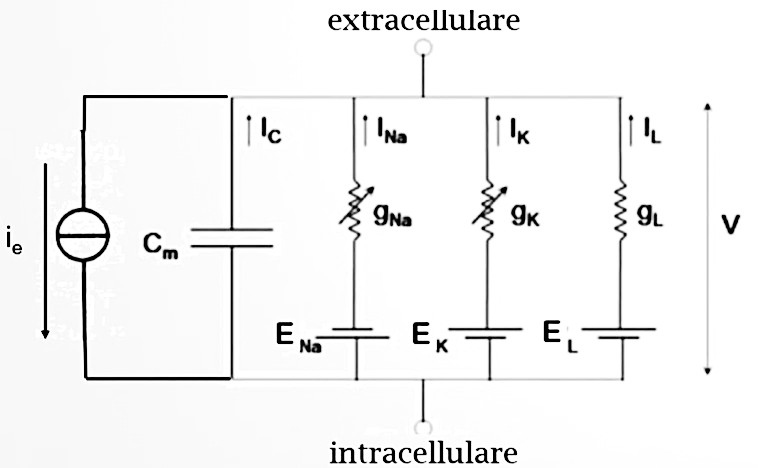
\includegraphics[width=0.80\textwidth]{images/image58.jpeg}
\end{figure}

I rami con conduttanza costante possono essere raggruppati in un unico \textbf{ramo di leakage}, formato da un resistore $g_L$ e un generatore $E_L$ (potenziale di riposo).

Se tutti i canali voltaggio-dipendenti sono chiusi e restano attivi solo i fenomeni di leakage, la membrana è in equilibrio e il potenziale è $E_L \approx -70$ mV.

La corrente di leakage è:
\[
i_L = g_L\,(V - E_L)
\]

\subsubsection{La membrana come circuito elettrico}

Tutti i fenomeni bioelettrici possono essere modellizzati con componenti circuitali:

\begin{itemize}
  \item \textbf{Differenza di potenziale ai lati della membrana = generatore di tensione}
  \item \textbf{Corrente ionica attraverso la membrana = corrente $I$ (che fluisce nel ramo)}
  \item \textbf{Canali ionici = resistori}
  \item \textbf{Doppio strato fosfolipidico = condensatore}
\end{itemize}

\textbf{ESEMPIO DI CIRCUITO EQUIVALENTE DI MEMBRANA}

Il circuito è composto da tanti rami in parallelo quanti sono i fenomeni da rappresentare: un ramo capacitivo, un ramo di leakage, e rami per i canali voltaggio-dipendenti (es. Na$^+$ e K$^+$) con conduttanze variabili.

\begin{figure}[htbp]
  \centering
  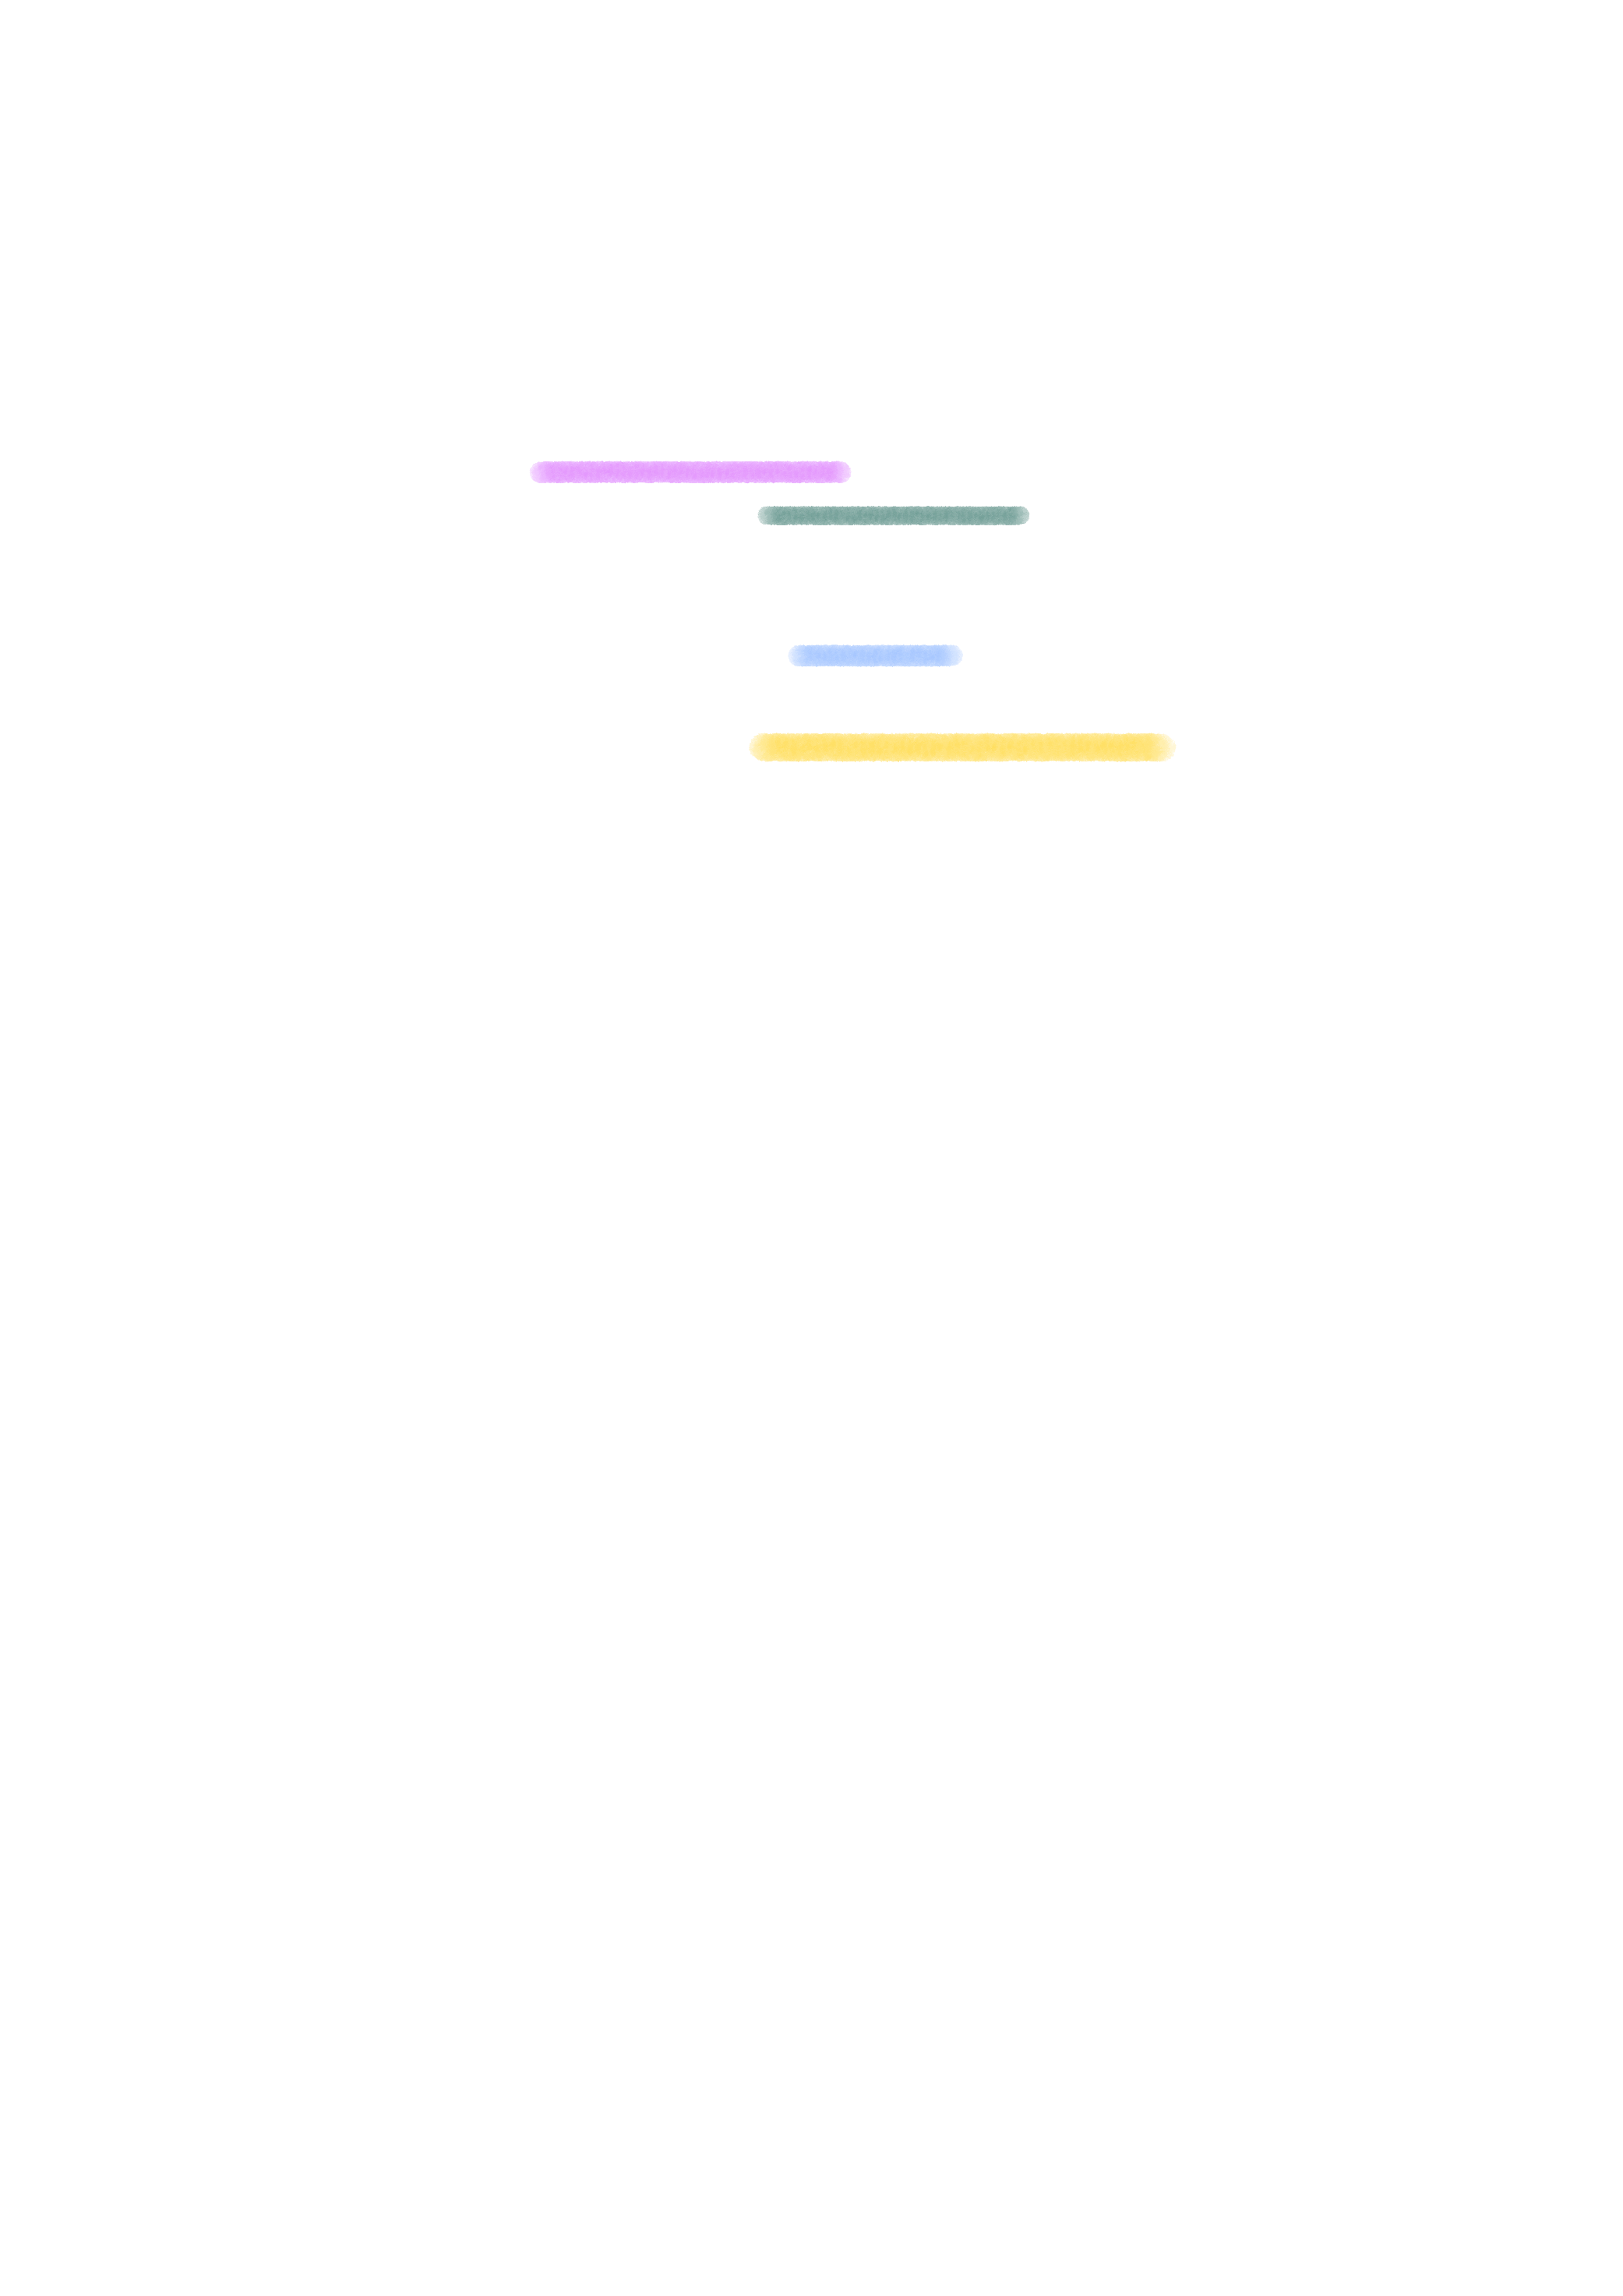
\includegraphics[width=0.80\textwidth]{images/image60.png}
\end{figure}

\begin{itemize}
  \item \textbf{Condensatore} $C_m$: capacità specifica di membrana.
  \item \textbf{Generatori} $E_{Na}$, $E_K$, $E_L$: potenziali di Nernst per Na$^+$, K$^+$ e potenziale di leakage.
  \item \textbf{Resistenze/conduttanze} $g_{Na}$, $g_K$, $g_L$: $g_{Na}$ e $g_K$ dipendono da $V$ e dal tempo, $g_L$ è costante.
  \item \textbf{Generatore di corrente esterna} $I_e$: corrente iniettata sperimentalmente o sinaptica.
\end{itemize}
Per Kirchhoff, la somma delle correnti è nulla:
\[
C_m\frac{dV}{dt} = -g_{Na}(V-E_{Na}) - g_K(V-E_K) - g_L(V-E_L) + I_e
\]

\section{2b. Il modello integra-e-spara}

\textbf{INTRODUZIONE -- quanto semplificare?}

Esistono diverse modellizzazioni del neurone, dal più semplice al più complesso. Il primo è il \textbf{modello integra-e-spara}: \textit{integrare} significa elaborare l'informazione ricevuta, \textit{sparare} indica generare un potenziale d'azione in modo rapido.

Domanda chiave: \textit{quanto è possibile semplificare?}

\begin{itemize}
  \item Nessun modello è una rappresentazione esatta della realtà.
  \item L'utilità è ciò che conta: un buon modello toglie ciò che non è essenziale.
  \item Ogni modello è un compromesso tra precisione e semplicità.
\end{itemize}

\textbf{MODELLO INTEGRA-E-SPARA}

Proposto da Lapicque nel 1907, è un modello estremamente semplificato che descrive bene il comportamento di base del neurone. All'epoca non si conoscevano i meccanismi molecolari, ma si sapeva che il neurone integra stimoli sotto soglia e “spara” un potenziale d'azione quando la depolarizzazione raggiunge una certa soglia.

\textit{Il neurone integra gli stimoli (variazioni del potenziale sotto soglia) e spara il potenziale d'azione non appena viene raggiunta la soglia.}

Il modello spiega solo i potenziali graduati (comportamento sotto soglia), non i meccanismi di generazione del potenziale d'azione.

\subsubsection{Meccanismi a soglia}

\begin{figure}[htbp]
  \centering
  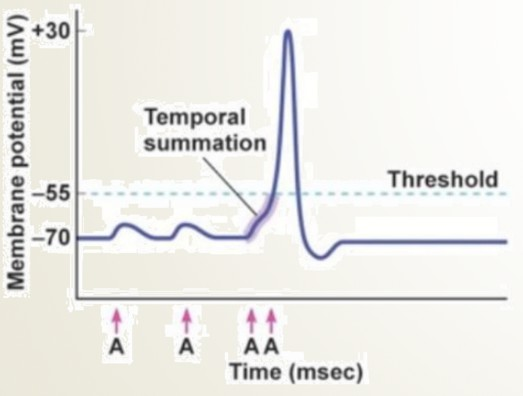
\includegraphics[width=0.80\textwidth]{images/image61.jpeg}
\end{figure}

Il modello ha due regioni di funzionamento:
\begin{itemize}
  \item \textbf{sotto soglia}: la membrana si comporta come un circuito RC;
  \item \textbf{sopra soglia}: si assume che venga generato un potenziale d'azione istantaneo (impulso).
\end{itemize}

\paragraph{Comportamento sotto soglia}
Si trascura l'effetto dei canali voltaggio-dipendenti (per piccole variazioni essi sono chiusi, conduttanza nulla). Il circuito si riduce a un condensatore $C_m$ in parallelo con una resistenza $R_m$ (che rappresenta il leakage) e un generatore di corrente $I_e$ (stimolazione).

\begin{figure}[htbp]
  \centering
  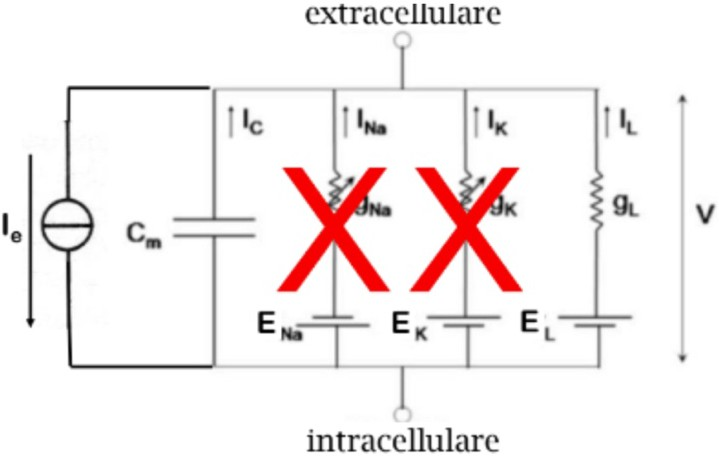
\includegraphics[width=0.80\textwidth]{images/image62.jpeg}
\end{figure}

Bilancio delle correnti:
\[
C_m\frac{dV}{dt} = -\frac{V - E_L}{R_m} + I_e
\]
Moltiplicando per $R_m$ e definendo la costante di tempo $\tau_m = R_m C_m$:
\[
\tau_m \frac{dV}{dt} = E_L - V + R_m I_e
\]

Quando $I_e = 0$ (assenza di stimolo):
\[
\tau_m \frac{dV}{dt} = E_L - V
\]
Soluzione:
\[
V(t) = E_L + (V_0 - E_L)\,e^{-t/\tau_m}
\]
dove $V_0$ è il potenziale iniziale. In assenza di corrente esterna, $V$ tende esponenzialmente a $E_L$ (potenziale di riposo).

\paragraph{Comportamento sopra soglia}
Quando il potenziale raggiunge la soglia $V_{th}$, il modello “spara” un potenziale d'azione. Lapicque, non potendo spiegare la dinamica rapida, assunse semplicemente che il potenziale venisse resettato a $V_{reset}$ e mantenuto costante per un breve periodo refrattario.

\begin{figure}[htbp]
  \centering
  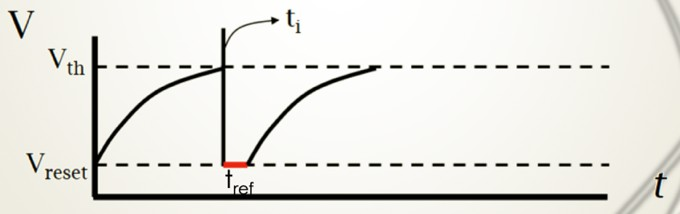
\includegraphics[width=0.80\textwidth]{images/image63.jpeg}
\end{figure}

\begin{figure}[htbp]
  \centering
  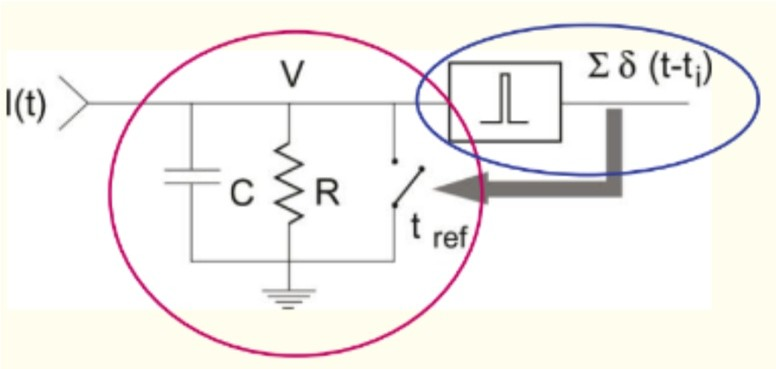
\includegraphics[width=0.80\textwidth]{images/image64.jpeg}
\end{figure}

\subsubsection{Potenziale di membrana}

Con una corrente iniettata positiva (simulando una sinapsi eccitatoria), il potenziale si depolarizza. Se la corrente non è sufficiente, non si raggiunge la soglia e il potenziale torna a riposo; se invece la corrente è abbastanza intensa, si raggiunge la soglia e il modello produce uno spike.

Il modello originale non includeva la refrattarietà dinamica, quindi la frequenza di scarica risultava lineare con la corrente iniettata, a differenza dei neuroni reali che mostrano adattamento.

\subsubsection{Refrattarietà assoluta e relativa (estensione del modello)}

Per correggere la linearità e introdurre l'adattamento, si può aggiungere una conduttanza inibitoria variabile nel tempo che si attiva dopo ogni spike:
\[
g_{ref}(t) = g_{ref}^0 \,\exp\!\left(-\frac{t - t_0}{\tau_{ref}}\right)
\]
dove $t_0$ è l'istante dell'ultimo spike. Questa conduttanza aumenta subito dopo lo spike (refrattarietà assoluta) e decade esponenzialmente (refrattarietà relativa), rendendo più difficile generare un nuovo potenziale d'azione.

\begin{figure}[htbp]
  \centering
  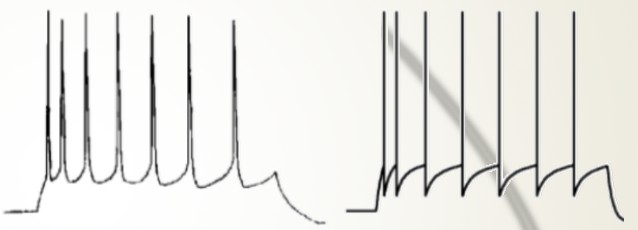
\includegraphics[width=0.80\textwidth]{images/image72.jpeg}
\end{figure}
\textit{Figura 1 -- Confronto dati reali / modello}

\begin{figure}[htbp]
  \centering
  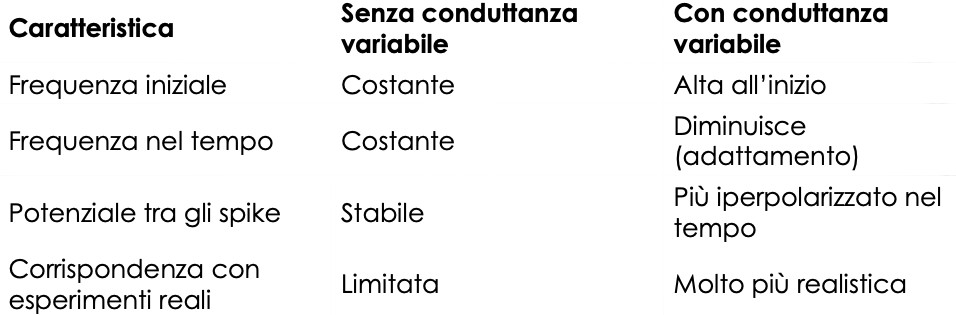
\includegraphics[width=0.80\textwidth]{images/image73.jpeg}
\end{figure}

\subsubsection{Conclusioni}

Il modello integra-e-spara, pur essendo molto semplice, riproduce la dinamica sotto soglia e la generazione di spike in modo qualitativamente corretto. Con l'aggiunta di una conduttanza di refrattarietà/adattamento si ottiene un buon accordo con i dati sperimentali. Tuttavia non descrive i meccanismi ionici alla base del potenziale d'azione; per questo si usano modelli più fisiologici come quello di Hodgkin-Huxley.

\section{2c. Modello di Hodgkin e Huxley}

\subsubsection{Complessità nei modelli di neurone}

Il modello di Hodgkin e Huxley (1952) descrive dinamicamente le correnti ioniche attraverso i canali voltaggio-dipendenti del Na$^+$ e del K$^+$, spiegando generazione e propagazione del potenziale d'azione. Fu sviluppato studiando l'assone gigante di calamaro (diametro $\sim$1 mm).

\subsubsection{Circuito equivalente di membrana}

\begin{figure}[htbp]
  \centering
  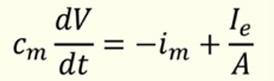
\includegraphics[width=0.80\textwidth]{images/image75.jpeg}
\end{figure}

Oltre al ramo capacitivo e a quello di leakage, si aggiungono due rami resistivi variabili per Na$^+$ e K$^+$, ognuno con un generatore ($E_{Na}$, $E_K$) e una conduttanza $g_{Na}(t,V)$, $g_K(t,V)$.

L'equazione del circuito (per unità di superficie) è:
\[
C_m\frac{dV}{dt} = -g_{Na}(V-E_{Na}) - g_K(V-E_K) - g_L(V-E_L) + I_e
\]

Le conduttanze $g_{Na}$ e $g_K$ sono prodotti di una conduttanza massima e una probabilità di apertura variabile.

\subsubsection{Conduttanza del canale K$^+$}

Il canale K$^+$ ha due stati (chiuso/aperto). La probabilità di apertura è modulata dalla variabile di attivazione $n$ (0$\le n \le 1$):
\[
g_K = \bar{g}_K \, n^4
\]
dove $\bar{g}_K$ è la conduttanza massima e l'esponente 4 fu determinato sperimentalmente (numero di subunità che devono attivarsi). La dinamica di $n$ è:
\[
\frac{dn}{dt} = \alpha_n(V)(1-n) - \beta_n(V)\,n
\]
ovvero, in forma equivalente:
\[
\frac{dn}{dt} = \frac{n_\infty(V) - n}{\tau_n(V)}
\]
con
\[
n_\infty(V) = \frac{\alpha_n}{\alpha_n+\beta_n}, \qquad
\tau_n = \frac{1}{\alpha_n+\beta_n}
\]
Le funzioni $\alpha_n(V),\beta_n(V)$ e quindi $n_\infty,\tau_n$ furono ottenute sperimentalmente con la tecnica del voltage clamp.

\begin{figure}[htbp]
  \centering
  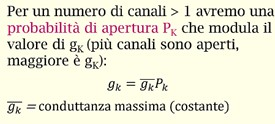
\includegraphics[width=0.80\textwidth]{images/image76.jpeg}
\end{figure}
\begin{figure}[htbp]
  \centering
  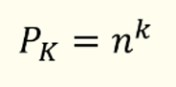
\includegraphics[width=0.80\textwidth]{images/image77.jpeg}
\end{figure}
\begin{figure}[htbp]
  \centering
  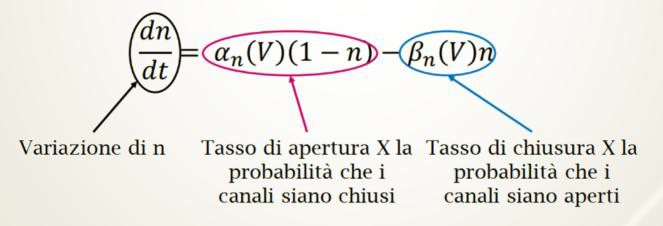
\includegraphics[width=0.80\textwidth]{images/image78.jpeg}
\end{figure}
\begin{figure}[htbp]
  \centering
  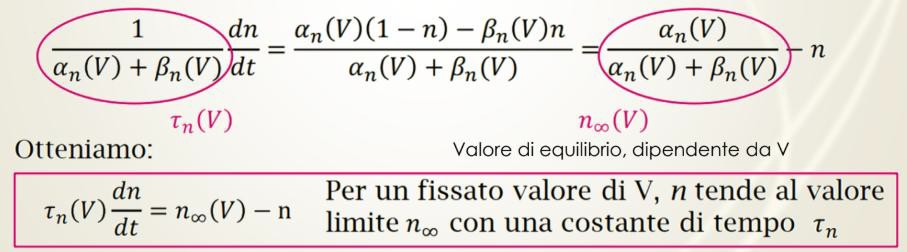
\includegraphics[width=0.80\textwidth]{images/image79.jpeg}
\end{figure}
\begin{figure}[htbp]
  \centering
  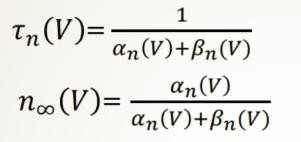
\includegraphics[width=0.80\textwidth]{images/image80.jpeg}
\end{figure}
\begin{figure}[htbp]
  \centering
  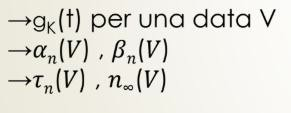
\includegraphics[width=0.80\textwidth]{images/image82.jpeg}
\end{figure}

\subsubsection{Voltage clamp}

La tecnica del voltage clamp mantiene il potenziale di membrana $V$ costante, permettendo di misurare le correnti ioniche in funzione del tempo senza l'effetto retroattivo della variazione di $V$ sulle conduttanze.

\begin{figure}[htbp]
  \centering
  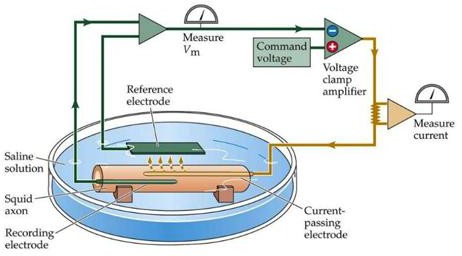
\includegraphics[width=0.80\textwidth]{images/image83.jpeg}
\end{figure}

Imponendo un gradino di potenziale (da un valore di holding a un valore di comando) si registra la corrente necessaria a mantenere $V$ costante, che è uguale ed opposta alla corrente ionica. Da queste misure si ricavano i parametri $\alpha$ e $\beta$.

\subsubsection{Conduttanza del canale Na$^+$}

Il canale Na$^+$ ha tre stati: chiuso, aperto, inattivo. Si descrive con due variabili:
\begin{itemize}
  \item $m$: probabilità che il canale \textbf{non sia chiuso} (attivazione);
  \item $h$: probabilità che \textbf{non sia inattivo} (inattivazione).
\end{itemize}
La conduttanza è:
\[
g_{Na} = \bar{g}_{Na}\, m^3 h
\]
Le dinamiche sono:
\[
\frac{dm}{dt} = \alpha_m(V)(1-m) - \beta_m(V)\,m, \qquad
\frac{dh}{dt} = \alpha_h(V)(1-h) - \beta_h(V)\,h
\]
oppure in forma $\tau$, $x_\infty$:
\[
\frac{dm}{dt} = \frac{m_\infty(V) - m}{\tau_m(V)},\qquad
\frac{dh}{dt} = \frac{h_\infty(V) - h}{\tau_h(V)}
\]

\begin{figure}[htbp]
  \centering
  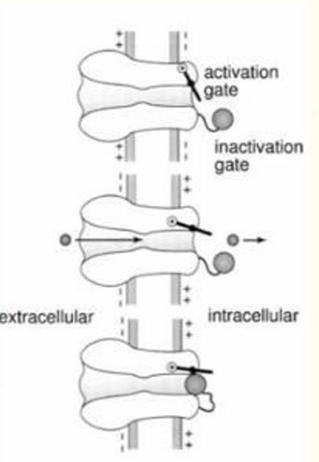
\includegraphics[width=0.80\textwidth]{images/image87.jpeg}
\end{figure}
\begin{figure}[htbp]
  \centering
  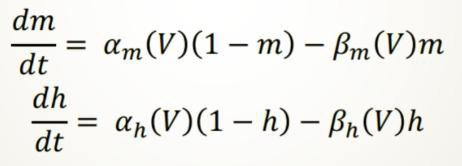
\includegraphics[width=0.80\textwidth]{images/image89.jpeg}
\end{figure}
\begin{figure}[htbp]
  \centering
  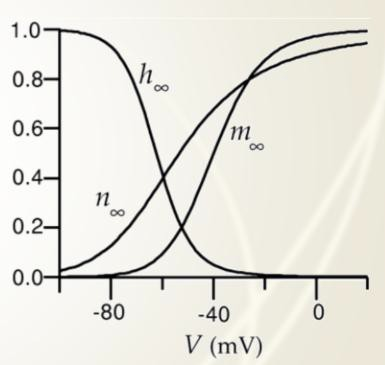
\includegraphics[width=0.80\textwidth]{images/image90.jpeg}
\end{figure}
\begin{figure}[htbp]
  \centering
  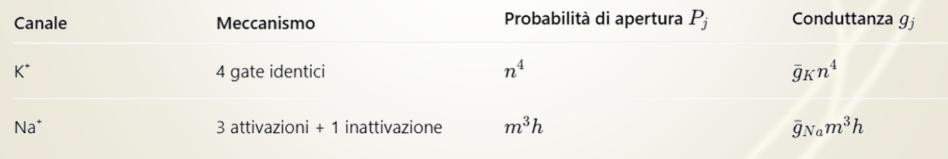
\includegraphics[width=0.80\textwidth]{images/image91.jpeg}
\end{figure}

\subsubsection{Modello completo di Hodgkin-Huxley}

Riassumendo, il modello è governato da quattro equazioni differenziali:
\[
C_m\frac{dV}{dt} = -\bar{g}_{Na}m^3h\,(V-E_{Na}) - \bar{g}_K n^4\,(V-E_K) - g_L(V-E_L) + I_e
\]
\[
\frac{dm}{dt} = \alpha_m(V)(1-m) - \beta_m(V)m
\]
\[
\frac{dh}{dt} = \alpha_h(V)(1-h) - \beta_h(V)h
\]
\[
\frac{dn}{dt} = \alpha_n(V)(1-n) - \beta_n(V)n
\]

Le funzioni $\alpha,\beta$ sono state determinate sperimentalmente da Hodgkin e Huxley.

\begin{figure}[htbp]
  \centering
  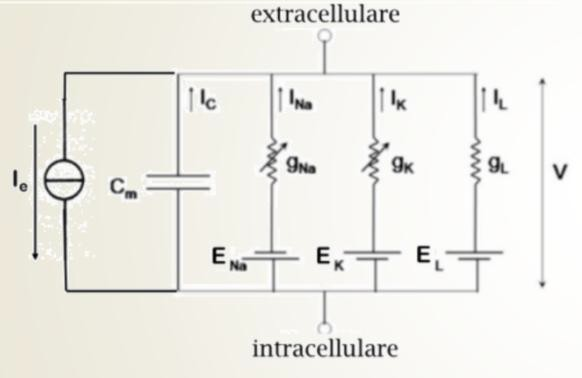
\includegraphics[width=0.80\textwidth]{images/image92.jpeg}
\end{figure}
\begin{figure}[htbp]
  \centering
  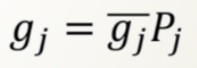
\includegraphics[width=0.80\textwidth]{images/image93.jpeg}
\end{figure}
\begin{figure}[htbp]
  \centering
  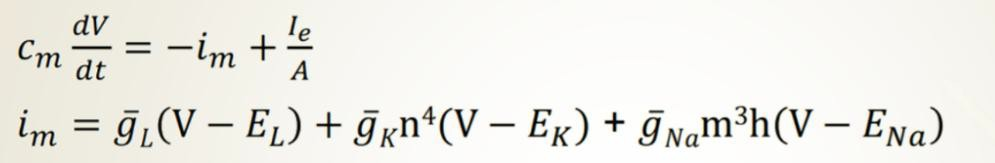
\includegraphics[width=0.80\textwidth]{images/image94.jpeg}
\end{figure}
\begin{figure}[htbp]
  \centering
  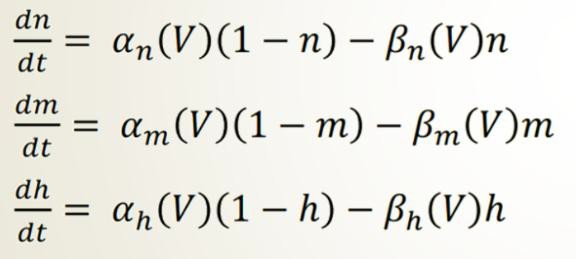
\includegraphics[width=0.80\textwidth]{images/image95.jpeg}
\end{figure}

\subsubsection{Dinamica di V e delle variabili}

All'equilibrio $m \approx 0$, $h \approx 1$, $n \approx 0$. Uno stimolo depolarizzante porta all'apertura dei canali Na$^+$ ($m$ aumenta), che produce una corrente entrante (depolarizzante, feedback positivo). Poi i canali Na$^+$ si inattivano ($h$ diminuisce) e contemporaneamente si attivano i canali K$^+$ ($n$ aumenta), generando una corrente uscente che ripolarizza la membrana. Il processo è autoalimentante per il Na$^+$ (serve l'inattivazione per fermarlo) e autolimitante per il K$^+$ (la ripolarizzazione chiude i canali).

\begin{figure}[htbp]
  \centering
  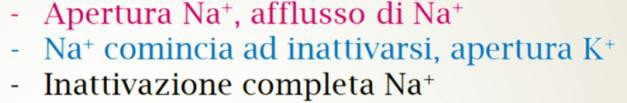
\includegraphics[width=0.80\textwidth]{images/image97.jpeg}
\end{figure}
\begin{figure}[htbp]
  \centering
  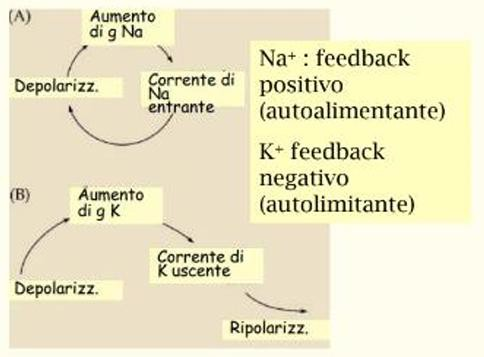
\includegraphics[width=0.80\textwidth]{images/image98.jpeg}
\end{figure}

\section{2d. Modello delle correnti sinaptiche}

\subsubsection{Sinapsi chimica richiami}

Il potenziale d'azione presinaptico provoca il rilascio di neurotrasmettitore, che si lega a recettori postsinaptici aprendo canali ionici. Si genera una corrente sinaptica $i_s$ che modifica il potenziale della cellula postsinaptica.

\subsubsection{Conduttanza sinaptica}

La corrente sinaptica per una sinapsi è:
\[
i_s = g_s(t)\,(V - E_s)
\]
dove $g_s(t)$ è la conduttanza sinaptica tempo-variante ed $E_s$ il potenziale di equilibrio del canale (0 mV per sinapsi eccitatorie, circa -80 mV per inibitorie).

La conduttanza è il prodotto di una conduttanza massima $\bar{g}_s$ e una probabilità di apertura $P(t)$:
\[
g_s(t) = \bar{g}_s \, P(t)
\]
$P(t)$ dipende dalla probabilità di rilascio presinaptico $P_{rel}$ e dalla probabilità di apertura postsinaptica $P_s$:
\[
P(t) = P_{rel}(t) \cdot P_s(t)
\]

\subsubsection{Probabilità di apertura postsinaptica $P_s(t)$}

Modelli tipici per $P_s(t)$ (in risposta a un singolo potenziale presinaptico):

\begin{itemize}
  \item \textbf{Funzione esponenziale} (apertura istantanea, chiusura esponenziale):
  \[
  P_s(t) = \exp\!\left(-\frac{t}{\tau_s}\right) \quad (t \ge 0)
  \]
  adatta per recettori ionotropici rapidi.
  \item \textbf{Funzione alfa} (salita e discesa con stessa costante di tempo):
  \[
  P_s(t) = \frac{t}{\tau_s}\,e^{-t/\tau_s}
  \]
  per recettori metabotropici o con cinetica più lenta.
  \item \textbf{Differenza di due esponenziali} (costanti di tempo diverse per salita e discesa):
  \[
  P_s(t) = B\,\Bigl(e^{-t/\tau_1} - e^{-t/\tau_2}\Bigr)
  \]
  molto flessibile.
\end{itemize}

\begin{figure}[htbp]
  \centering
  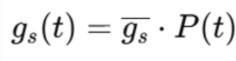
\includegraphics[width=0.80\textwidth]{images/image100.jpeg}
\end{figure}
\begin{figure}[htbp]
  \centering
  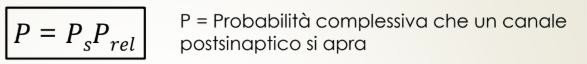
\includegraphics[width=0.80\textwidth]{images/image101.jpeg}
\end{figure}
\begin{figure}[htbp]
  \centering
  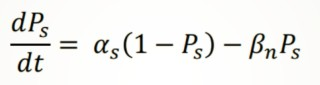
\includegraphics[width=0.80\textwidth]{images/image102.jpeg}
\end{figure}
\begin{figure}[htbp]
  \centering
  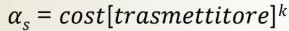
\includegraphics[width=0.80\textwidth]{images/image103.jpeg}
\end{figure}
\begin{figure}[htbp]
  \centering
  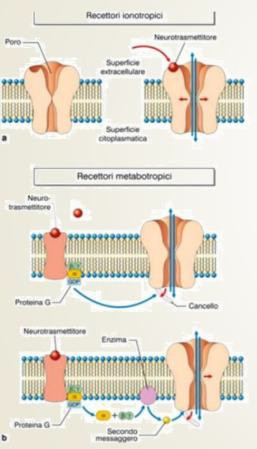
\includegraphics[width=0.80\textwidth]{images/image104.jpeg}
\end{figure}
\begin{figure}[htbp]
  \centering
  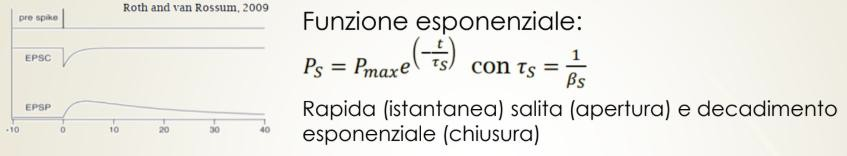
\includegraphics[width=0.80\textwidth]{images/image105.jpeg}
\end{figure}
\begin{figure}[htbp]
  \centering
  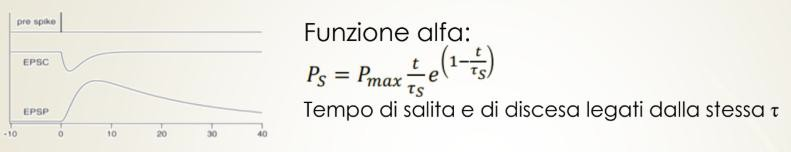
\includegraphics[width=0.80\textwidth]{images/image106.jpeg}
\end{figure}
\begin{figure}[htbp]
  \centering
  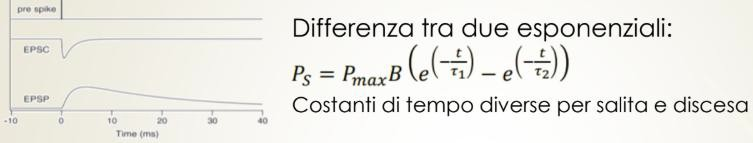
\includegraphics[width=0.80\textwidth]{images/image107.jpeg}
\end{figure}

\subsubsection{Probabilità di rilascio presinaptico $P_{rel}$}

In condizioni normali $P_{rel}$ è circa costante. Con stimolazioni ripetute si osservano:
\begin{itemize}
  \item \textbf{Depressione sinaptica}: $P_{rel}$ diminuisce a ogni stimolo (esaurimento vescicole). Modello: $P_{rel} \leftarrow f_D \cdot P_{rel}$ con $0<f_D<1$.
  \item \textbf{Facilitazione sinaptica}: $P_{rel}$ aumenta per accumulo di calcio residuo. Modello: $P_{rel} \leftarrow P_{rel} + f_F$ con $f_F>0$.
\end{itemize}

\begin{figure}[htbp]
  \centering
  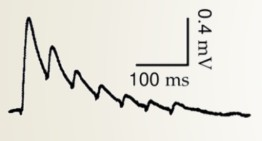
\includegraphics[width=0.80\textwidth]{images/image108.jpeg}
\end{figure}
\begin{figure}[htbp]
  \centering
  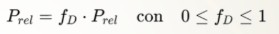
\includegraphics[width=0.80\textwidth]{images/image109.jpeg}
\end{figure}
\begin{figure}[htbp]
  \centering
  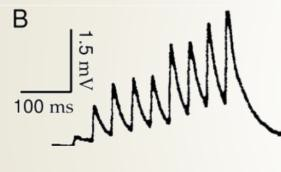
\includegraphics[width=0.80\textwidth]{images/image110.jpeg}
\end{figure}

\subsubsection{Correnti sinaptiche nel modello}

Inserendo un ramo sinaptico per ogni sinapsi, la corrente totale sinaptica (eccitatoria + inibitoria) è:
\[
i_{syn} = \sum_k g_{s,k}(t)\,(V - E_{s,k})
\]
che si aggiunge all'equazione di membrana. Così si possono modellare reti di neuroni.

\begin{figure}[htbp]
  \centering
  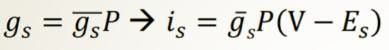
\includegraphics[width=0.80\textwidth]{images/image112.jpeg}
\end{figure}
\begin{figure}[htbp]
  \centering
  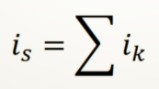
\includegraphics[width=0.80\textwidth]{images/image113.jpeg}
\end{figure}
\begin{figure}[htbp]
  \centering
  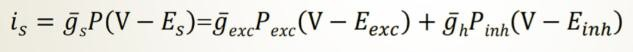
\includegraphics[width=0.80\textwidth]{images/image114.jpeg}
\end{figure}
\begin{figure}[htbp]
  \centering
  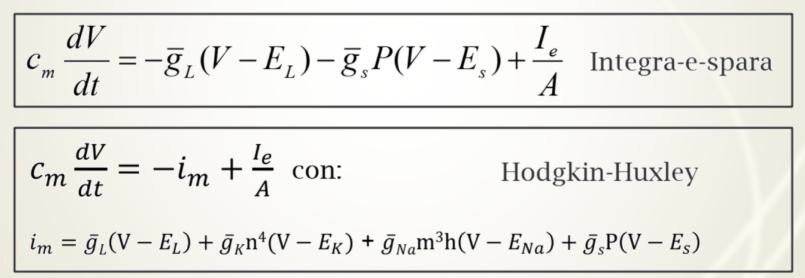
\includegraphics[width=0.80\textwidth]{images/image115.jpeg}
\end{figure}

\chapter{Modelli multicompartimentali della membrana neuronale}

\section{3a. Modello di propagazione intracellulare}

Finora abbiamo ignorato la \textbf{dimensione spaziale}, scelta accettabile per descrivere i meccanismi di base (sinapsi, potenziale d'azione, sommazione temporale). Tuttavia, non è sufficiente quando si vogliono spiegare fenomeni come sommazione spaziale, propagazione lungo la membrana e conduzione del potenziale d'azione.

Anche se la struttura neuronale reale è tridimensionale e complessa, dendriti e assone possono essere \textbf{approssimati come cilindri}, o come combinazioni di cilindri $\Rightarrow$ questo permette di ridurre il problema alla sola dimensione \textbf{longitudinale ($x$)}: il potenziale di membrana $V$ dipenderà quindi dal tempo $t$ e dalla posizione $x$.

\begin{figure}[htbp]
  \centering
  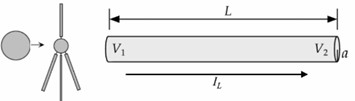
\includegraphics[width=0.80\textwidth]{images/image116.jpeg}
\end{figure}

\subsubsection{Propagazione passiva}

Il soma è rappresentato come un cilindro singolo, mentre l'albero dendritico come una serie di cilindri collegati.

Se in un punto della membrana si genera una variazione del potenziale ($V_1$), questa si ripercuote anche nelle zone vicine ($V_2$) per la propagazione passiva.

La depolarizzazione locale crea un gradiente di cariche all'interno del cilindro: gli ioni si spostano lungo questo gradiente generando correnti intracellulari longitudinali che modificano il potenziale nei punti vicini. Durante questo movimento, la corrente incontra una resistenza longitudinale ($R_L$), che:
\begin{itemize}
  \item cresce con la lunghezza del cilindro,
  \item diminuisce con l'aumentare della sezione,
  \item è determinata da una resistenza specifica intracellulare $r_L$, tipicamente molto elevata (ordine dei k$\Omega$$\cdot$mm).
\end{itemize}

\begin{figure}[htbp]
  \centering
  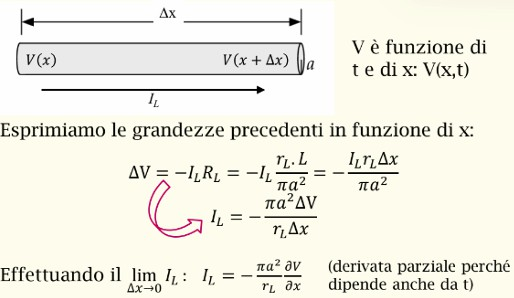
\includegraphics[width=0.80\textwidth]{images/image117.jpeg}
\end{figure}

\subsubsection{Teoria dei cavi}

Permette di descrivere il potenziale di membrana come funzione del tempo $t$ e della posizione $x$ lungo un cilindro (dendrite o assone). Nasce dall'analogia tra un neurone e un cavo elettrico, adattata alle caratteristiche della membrana.

Considerando un segmento $\Delta x$ di cilindro, la differenza di potenziale tra gli estremi è legata alla corrente longitudinale e alla resistenza interna. Passando al limite $\Delta x \to 0$, si ottiene l'equazione dei telegrafisti:
\[
\frac{1}{r_L}\frac{\partial^2 V}{\partial x^2} = c_m\frac{\partial V}{\partial t} + i_m
\]
dove $i_m$ è la corrente di membrana per unità di superficie (include correnti ioniche e stimoli esterni). Per un cavo cilindrico di raggio $a$:
\[
\frac{a}{2r_L}\frac{\partial^2 V}{\partial x^2} = c_m\frac{\partial V}{\partial t} + i_m
\]

Le condizioni al contorno tipiche sono: continuità di $V$, conservazione della corrente ai nodi, e corrente uscita nulla alle estremità (estremità sigillate).

\begin{figure}[htbp]
  \centering
  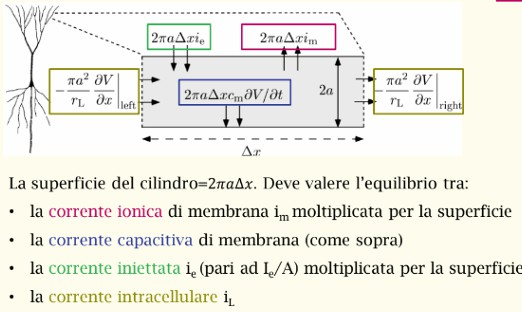
\includegraphics[width=0.80\textwidth]{images/image118.jpeg}
\end{figure}
\begin{figure}[htbp]
  \centering
  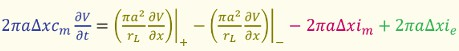
\includegraphics[width=0.80\textwidth]{images/image119.jpeg}
\end{figure}
\begin{figure}[htbp]
  \centering
  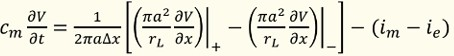
\includegraphics[width=0.80\textwidth]{images/image120.jpeg}
\end{figure}
\begin{figure}[htbp]
  \centering
  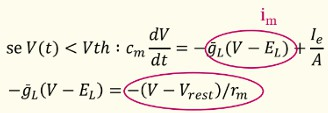
\includegraphics[width=0.80\textwidth]{images/image122.jpeg}
\end{figure}

Per la propagazione passiva (sotto soglia, canali voltaggio-dipendenti chiusi) si utilizza il modello RC lineare:
\[
i_m = g_L\,(V - E_L)
\]
e l'equazione dei cavi diventa lineare.

\section{3b. Modello multi-compartimentale di propagazione del potenziale d'azione}

\subsubsection{Modelli multi-compartimentali}

Si discretizza la coordinata spaziale: il neurone è suddiviso in tanti compartimenti, ciascuno abbastanza piccolo da considerare il potenziale uniforme al suo interno. Ogni compartimento è modellato con un circuito di membrana (es. Hodgkin-Huxley) e i compartimenti sono collegati da resistenze longitudinali che rappresentano la propagazione passiva.

\begin{figure}[htbp]
  \centering
  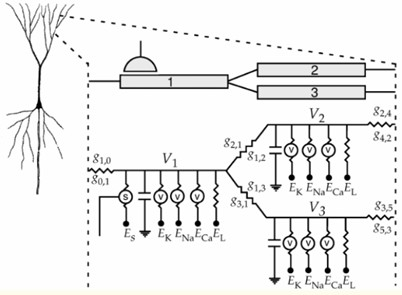
\includegraphics[width=0.80\textwidth]{images/image125.jpeg}
\end{figure}

\begin{itemize}
  \item Compartimento del bottone sinaptico: rami sinaptici + canali voltaggio-dipendenti.
  \item Compartimenti internodali: solo canali voltaggio-dipendenti (o solo leakage nei tratti mielinizzati).
\end{itemize}

\begin{figure}[htbp]
  \centering
  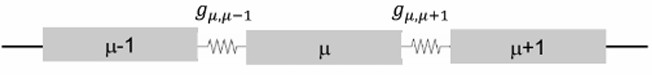
\includegraphics[width=0.80\textwidth]{images/image126.jpeg}
\end{figure}
\begin{figure}[htbp]
  \centering
  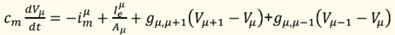
\includegraphics[width=0.80\textwidth]{images/image127.jpeg}
\end{figure}

L'equazione per il compartimento $k$ è:
\[
C_m\frac{dV_k}{dt} = -i_{m,k} + \frac{V_{k-1} - V_k}{R_{k-1,k}} + \frac{V_{k+1} - V_k}{R_{k,k+1}} + I_{e,k}
\]
dove $R_{k-1,k}$ è la resistenza di raccordo tra i compartimenti.

\subsubsection{Propagazione continua}

Negli assoni non mielinizzati, ogni compartimento è di tipo Hodgkin-Huxley. La propagazione avviene per rigenerazione punto a punto: la depolarizzazione in un compartimento attiva i canali Na$^+$ nel compartimento adiacente.

\begin{figure}[htbp]
  \centering
  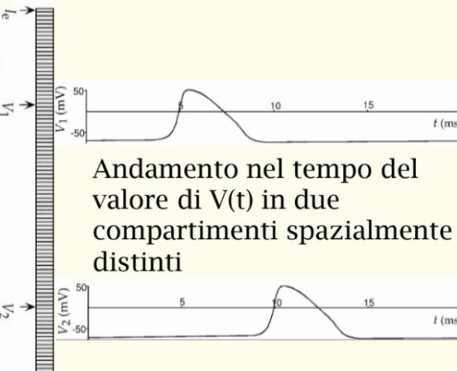
\includegraphics[width=0.80\textwidth]{images/image130.jpeg}
\end{figure}

Graficamente, fissato un istante $t$, il potenziale $V$ lungo l'assone mostra un picco nel punto dove in quell'istante si sta verificando il potenziale d'azione, preceduto da una zona già ripolarizzata e seguito da una zona ancora a riposo.

\subsubsection{Propagazione saltatoria}

Negli assoni mielinizzati, la guaina mielinica isola la membrana. I canali voltaggio-dipendenti sono concentrati solo nei nodi di Ranvier, mentre i tratti internodali sono modellati come pura capacità e resistenza di leakage molto alta (bassa conduttanza).

Il circuito equivalente alterna:
\begin{itemize}
  \item \textbf{nodi}: modello di Hodgkin-Huxley (o una sua semplificazione);
  \item \textbf{segmenti mielinizzati}: capacità e resistenza di membrana molto elevata.
\end{itemize}
La corrente generata in un nodo si propaga passivamente fino al nodo successivo, dove, se la depolarizzazione supera la soglia, rigenera un nuovo potenziale d'azione. Il segnale sembra “saltare” da un nodo all'altro, con un grande aumento della velocità di conduzione.

\begin{figure}[htbp]
  \centering
  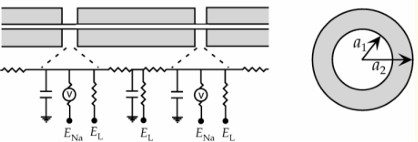
\includegraphics[width=0.80\textwidth]{images/image132.jpeg}
\end{figure}
\begin{figure}[htbp]
  \centering
  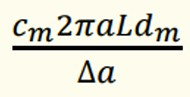
\includegraphics[width=0.80\textwidth]{images/image133.jpeg}
\end{figure}
\begin{figure}[htbp]
  \centering
  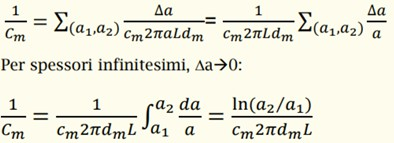
\includegraphics[width=0.80\textwidth]{images/image134.jpeg}
\end{figure}

\subsubsection{Schema riassuntivo: propagazione passiva, continua e saltatoria}

\begin{table}[htbp]
\centering
\begin{tabular}{p{3cm}p{4.5cm}p{4.5cm}}
\toprule
\textbf{Caratteristica} & \textbf{Propagazione passiva} & \textbf{Propagazione continua} \\
\midrule
Modello & Integra-e-spara sotto soglia & Hodgkin-Huxley \\
Correnti & Solo leakage (canali volt.-dip. chiusi) & Canali voltaggio-dipendenti (Na$^+$, K$^+$) \\
Equazione & Cavo lineare & Cavo con conduttanze variabili \\
Risultato & Attenuazione passiva & Rigenerazione attiva continua \\
Esempio & Potenziali graduati & Assone amielinico \\
\bottomrule
\end{tabular}
\end{table}

\begin{table}[htbp]
\centering
\begin{tabular}{p{3cm}p{4.5cm}p{4.5cm}}
\toprule
\textbf{Caratteristica} & \textbf{Propagazione saltatoria} \\
\midrule
Modello & Ibrido: HH nei nodi, cavo passivo nei tratti mielinizzati \\
Struttura & Nodi di Ranvier + guaina mielinica \\
Modello fisico & Condensatori in serie + alta resistenza (cilindri concentrici) \\
Capacità equivalente & Ridotta, aumenta la velocità \\
Conduzione & Velocità elevata, bassa dissipazione \\
Unidirezionalità & Garantita dai canali Na$^+$ (refrattarietà) \\
\bottomrule
\end{tabular}
\end{table}

\chapter{Modelli di encoding e decoding neuronale}

\section{4a. Funzione di risposta neuronale e frequenza di scarica}

\subsubsection{Introduzione}

Il neurone è visto come una scatola nera (Neural Spiking System) che trasforma un input (caratteristica di uno stimolo) in un output (treno di spike). L'encoding descrive la risposta neuronale in funzione dello stimolo; il decoding cerca di risalire allo stimolo a partire dalla risposta.

A causa della variabilità biologica, il legame stimolo-risposta è di tipo probabilistico.

\textbf{Treni di impulsi e funzione di risposta}

La sequenza di spike in un trial di durata $T$ si rappresenta come somma di delta di Dirac:
\[
\rho(t) = \sum_{i=1}^{n} \delta(t - t_i)
\]
dove $t_i$ sono gli istanti degli $n$ spike. $\rho(t)$ è la \textbf{funzione di risposta neuronale}.

\subsubsection{Ipotesi della codifica in frequenza}

L'informazione è codificata nella \textbf{frequenza di scarica} (firing rate) $r$, non nell'ampiezza o nella forma del potenziale d'azione. La frequenza influenza la sommazione temporale a livello postsinaptico.

\subsubsection{Frequenza di scarica}

Due definizioni:
\begin{enumerate}
  \item \textbf{Media sul trial}: $r = \frac{n}{T} = \frac{1}{T}\int_0^T \rho(t)\,dt$ (spike/s = Hz).
  \item \textbf{Frequenza istantanea (finestrata)}: si divide il trial in intervalli $\Delta t$ e si calcola $r(t) = \frac{n_{\Delta t}}{\Delta t}$. Per migliorare la risoluzione si può far scorrere la finestra o usare nuclei di convoluzione (boxcar, gaussiana, causale). Mediando su molti trial si ottiene il \textbf{Peri-Stimulus Time Histogram} (PSTH), che approssima la probabilità di scarica $r(t)\Delta t$.
\end{enumerate}

\subsubsection{Calcolo di $r(t)$}

Vari approcci per stimare $r(t)$ da un singolo trial (o mediati):
\begin{enumerate}
  \item Finestre disgiunte (risoluzione temporale bassa).
  \item Finestra mobile rettangolare (risoluzione migliore ma introduce correlazione).
  \item Finestra gaussiana (più liscia, ma simmetrica → risposta anticipata).
  \item Finestra causale ($=0$ per $t<0$) → risposta ritardata, fisiologicamente più corretta.
\end{enumerate}

\section{4b. Curve di Tuning}

\subsubsection{Introduzione}

Si considera uno stimolo stazionario caratterizzato da un parametro $s$. La frequenza di scarica media $\langle r \rangle$ (mediata su più trial) è una funzione $f(s)$, detta \textbf{curva di tuning}.

Costruzione:
\begin{enumerate}
  \item Identificare il parametro $s$ dello stimolo.
  \item Far variare $s$ sistematicamente ed eseguire più trial per ogni valore.
  \item Registrare l'attività neuronale (extracellulare).
  \item Calcolare $\langle r \rangle$ per ogni $s$.
  \item Riportare i punti $(s,\langle r \rangle)$ e fittare una funzione matematica.
\end{enumerate}

\subsubsection{Esempi}
\begin{itemize}
  \item \textbf{Orientamento di una barra luminosa} (V1): curva gaussiana centrata sull'orientamento preferito.
  \item \textbf{Direzione del movimento del braccio} (corteccia motoria): $f(s) = r_0 + (r_{max}-r_0)\cos(s - s_{max})$, con $s$ angolo di movimento.
  \item \textbf{Distanza di un oggetto} (visione binoculare): neuroni “far-tuned” che rispondono solo per oggetti oltre una certa distanza (curva sigmoidale).
\end{itemize}

\section{4c. Decoding neuronale}

Si cerca di stimare lo stimolo $s$ a partire dalla risposta $r$. Poiché la relazione non è invertibile univocamente, si usa un approccio probabilistico.

\textbf{Esempio}: neurone sensibile alla direzione del movimento (preferita +, opposta --). Si costruiscono gli istogrammi di $r$ per i due stimoli a diversi livelli di coerenza. Si definisce una soglia $z$: se $r \ge z$ si classifica come direzione +, altrimenti --.

\textbf{Valutazione}: $\alpha(z) = P(\text{falso positivo})$, $\beta(z) = P(\text{vero positivo})$. La curva ROC mostra $\beta$ vs $\alpha$ al variare di $z$. L'area sotto la curva (AUC) misura la capacità discriminativa del neurone: AUC $\sim 1$ indica prestazioni ottime, AUC $\sim 0.5$ caso.

Nel caso della direzione del movimento, l'AUC cresce con la coerenza, mostrando che anche un singolo neurone può discriminare la direzione in modo simile al comportamento dell'animale.

\section{Applicazioni dell'encoding e decoding neuronale}

Le interfacce cervello-computer (BCI) utilizzano modelli di decoding per tradurre l'attività neuronale in comandi per protesi motorie o sensoriali, bypassando le vie nervose danneggiate.

\chapter{Modelli di reti cerebrali}

\section{5a. Reti di neuroni e applicazioni}

\textbf{Complessità e connettività}

Il cervello umano contiene circa 86 miliardi di neuroni, fittamente interconnessi (10$^3$--10$^5$ sinapsi per neurone). Le fibre nervose formano una struttura ordinata di reti, studiabile con tecniche invasive (istologia) e non invasive (risonanza magnetica pesata in diffusione).

\textbf{Modelli di rete}

\begin{itemize}
  \item \textbf{Spiking models} (es. Hodgkin-Huxley, integra-e-spara): descrivono nei minimi dettagli la dinamica del potenziale di membrana, includendo tutti i canali ionici e le sinapsi. Sono molto accurati ma computazionalmente onerosi, adatti a piccole reti.
  \item \textbf{Firing models} (encoding-decoding): modelli a scatola nera che collegano direttamente lo stimolo alla frequenza di scarica. Ignorano la dinamica sub-millisecondo ma sono molto efficienti per grandi popolazioni di neuroni. Incorporano la variabilità in modo probabilistico.
\end{itemize}

\textbf{Vantaggi e limiti}

Gli spiking models sono più fedeli alla fisiologia e spiegano i meccanismi, ma richiedono molte risorse di calcolo e parametri. I firing models sono leggeri, adatti a simulazioni di larga scala, ma meno precisi e non spiegano i meccanismi sottostanti.

\section{Applicazioni dei modelli computazionali dei sistemi neurali}

\begin{itemize}
  \item \textbf{Reti neurali biomimetiche spiking}: implementate su hardware (FPGA) per emulare circuiti neurali reali, con plasticità sinaptica. Possibili future neuroprotesi.
  \item \textbf{Neuroprotesi}:
    \begin{itemize}
      \item \textit{Sensoriali}: impianti cocleari, protesi visive (stimolazione retinica o corticale).
      \item \textit{Motorie}: arti robotici, stimolazione elettrica funzionale (FES) per ripristinare il controllo muscolare. Richiedono decodifica dell'attività corticale.
    \end{itemize}
  \item \textbf{The Human Brain Project}: mira a ricostruire il cervello umano tramite modelli computazionali.
  \item \textbf{Reti neurali artificiali}: ispirate ai neuroni biologici, sono alla base dell'IA moderna.
\end{itemize}

\textbf{Conclusioni}

I modelli quantitativi non solo imitano la natura, ma aiutano a comprendere i meccanismi fisiologici, formalizzare ipotesi, integrare dati e fare previsioni. Sono strumenti fondamentali per le neuroscienze teoriche e le applicazioni neurotecnologiche.

\end{document}